\documentclass[twoside,english,a4paper,12pt]{uiofysmaster}
\usepackage{lmodern}
\usepackage[T1]{fontenc}
\usepackage[utf8]{inputenc}
% \usepackage[top=1.5in, bottom=1.5in, left=1in, right=1in]{geometry} % Correct geometry is in uiofysmaster

% ----  biblatex ---- %
\usepackage[english]{babel}
\usepackage{csquotes} % required by {babel} (or biblatex?)
\usepackage[backend=biber, sorting=nyt, style=numeric]{biblatex} % Note that "sorting=none" is NOT the same as leaving the field blank, "sorting=none" means "sorting=citeorder".
% About DATES:
% The date fields date, origdate, eventdate, and urldate require a date specification in yyyy-mm-dd format. Date ranges are given as yyyy-mm-dd/yyyy-mm-dd. Partial dates are valid provided that date components are omitted at the end only. You may specify an open ended date range by giving the range separator and omitting the end date (e. g., yyyy/).
\bibliography{bibliography/JabRef_database,bibliography/Master}

% ---- Code syntax highlighting ---- %
% \usepackage[scaled=0.8]{beramono}  % Better monospaced font, nice ~ and ^
\usepackage[scale=0.85]{droidmono}

% Order: float - (fix \listoflistings) - hyperref - minted
\usepackage{float}

% Fix listoflistings (need to do this before loading hyperref)
% Fix \listoflistings
\usepackage{etoolbox}
% \newfloat{listing}{h}{lol} % Not necessary
\makeatletter
\patchcmd{\@chapter}%
 {\addtocontents{lof}}%
 {\addtocontents{lol}{\protect\addvspace{10pt}}%  % <-- "lol" is the extension minted use
  \addtocontents{lof}}%
\makeatother

% FIX LIST OF LISTINGS: 
% http://tex.stackexchange.com/a/58498/31078
% http://tex.stackexchange.com/questions/14856/change-spacing-between-elements-in-newfloat-listof/14867#14867
% http://tex.stackexchange.com/questions/139533/using-listing-with-minted-gets-wrong-listoflistings


% Load hyperref after fixing listoflistings
\usepackage{hyperref}
\hypersetup{
    colorlinks,
    citecolor=blue,
    filecolor=black,
    linkcolor=black,
    urlcolor=blue,
}
\urlstyle{same}


% Finally load minted
\usepackage[chapter]{minted} % Option [chapter] has to do with \listoflistings numbering. Alternative is ``section''
% Need to load the float package before hyperref, so hyperref detects and patches it, so when we load minted later it uses the patched \newfloat (minted loads float). 
% More info here: http://tex.stackexchange.com/questions/19371/minteds-listing-environment-with-hyperref-and-caption-package-together

\usemintedstyle{colorful}
\definecolor{codebg}{rgb}{0.95,0.95,0.95}
\newminted[cppcode]{mdcpp}{ % can use \newminted{cpp} to replace default ``cpp'', gives the same result
    mathescape,
%     frame=lines,
%     framesep=2mm,
    bgcolor = codebg,
%     fontsize = \small,
    fontsize = \footnotesize,
%     fontfamily = courier
} 
% usage: \begin{cppcode}
% use \begin{cppcode*}{<extra options>} if you want to add extra options on the fly

% More options:
% \renewcommand\listingscaption{Program code}
% \renewcommand\listoflistingscaption{List of program codes}

% FIX LIST OF LISTINGS: 
% http://tex.stackexchange.com/a/58498/31078
% http://tex.stackexchange.com/questions/14856/change-spacing-between-elements-in-newfloat-listof/14867#14867
% http://tex.stackexchange.com/questions/139533/using-listing-with-minted-gets-wrong-listoflistingscaption



% ----  Draft stuff (remove before final version) ---- %
\usepackage[colorinlistoftodos,color=black!20]{todonotes}
\usepackage{xcolor}
\newcommand{\orangebox}[1]{
    \fcolorbox{black}{orange}{
        \begin{minipage}{\textwidth}
            #1
        \end{minipage}
    }
}
\usepackage{soulutf8}       % To highlight stuff (when using utf8), using \hl{}. Also has \st{} for strikethrough. Doesn't work that well with equations...
\usepackage{lipsum}

% ---- Images ---- %
\usepackage{graphicx}
\usepackage{svg}            % To include .svg vector graphics directly using \includesvg (will automatically compile/convert the images to .pdf+.pdf_tex using Inkscape). 
                            % NEEDS ``pdflatex --shell-escape'' !!!
                            
\setsvg{%                   % conversion options for svg package
    inkscape = inkscape -z -D,%
    pretex = \footnotesize%
}

% The subfigure and subfig packages are deprecated and shouldn't be used any more: 
% http://tex.stackexchange.com/questions/144782/subfigure-and-subfig-packages-deprecated
% the svg-package originally uses subfig, but replacing subfig with subcaption seems to work
\usepackage{subcaption}     % \begin{subfigure}, \subcaption{}, and \subcaptionbox{}

% ---- Fix unicode stuff ---- %
\DeclareUnicodeCharacter{2212}{-}   % Unicode 'MINUS SIGN' (U+2212) that matplotlib uses for minus on axis tick labes

% ---- Formatting ---- %
% skip line instead of indent on new paragraph
% \setlength{\parskip}{11pt}
% \setlength{\parindent}{0mm}
\newlength{\oldparindent}
\setlength{\oldparindent}{\parindent} % doesn't work?
\usepackage[parfill]{parskip} % The option parfill is a useful addition: it avoids that a paragraph ends almost flush right. So, paragraphs could easier be distinguished.

% ---- Floats ---- %
% With \renewcommand{\floatpagefraction}{.8}% I was able to specify that only pages with more than 80% of floats, will become pure float-only pages. The default is 0.6 so if a figure consumes 60% of the page it will get its own float-page.
\renewcommand{\floatpagefraction}{.8}

% There are four counters that control how many floats can go into areas:
% totalnumber (default 3) is the maximum number of floats on a text (!) page
% topnumber (default 2) is the maximum number of floats in the top area
% bottomnumber (default 1) is the maximum number of floats in the bottom area
% dbltopnumber (default 2) is the maximum number of full sized floats in two-colum mode going above the text columns.
\setcounter{totalnumber}{6}
\setcounter{topnumber}{4}
\setcounter{bottomnumber}{2}

%TODO:
% Consider increasing +- ranges?
% Show defaults using \showthe\textfloatsep or \the\textfloatsep
% See here for defaults: http://tex.stackexchange.com/a/23316/31078
% See image here for illustration of space: http://tex.stackexchange.com/a/60479/31078
% Defaults for uiofysmaster using default font size
% \floatsep:        12.0pt plus 2.0pt minus 4.0pt
% \textfloatsep:    20.0pt plus 2.0pt minus 4.0pt
% \intextsep:       14.0pt plus 4.0pt minus 4.0pt
% \dbltextfloatsep: 20.0pt plus 2.0pt minus 4.0pt
% \dblfloatsep:     14.0pt plus 2.0pt minus 4.0pt
% \setlength{\textfloatsep}{14.0pt plus 8.0pt minus 0.0pt} % 20.0pt plus 2.0pt minus 4.0pt
% \setlength{\intextsep}{8.0pt plus 6.0pt minus 0.0pt} % 14.0pt plus 4.0pt minus 4.0pt 
% \setlength{\floatsep}{8.0pt plus 4.0pt minus 0.0pt} % 12.0pt plus 2.0pt minus 4.0pt

% ---- Captions ---- %
% \usepackage{caption} % Loaded by uiofysmaster
\captionsetup[table]{width=.9\textwidth,position=above}
\captionsetup[figure]{width=.9\textwidth,position=below}
\captionsetup[listing]{width=.9\textwidth,position=below}
% \captionsetup{font=small,labelfont=bf} % In uiofysmaster
\captionsetup[subfigure]{position=below}

% See image here for illustration of space: http://tex.stackexchange.com/a/60479/31078
% See here for defaults: http://tex.stackexchange.com/a/23316/31078
% Show defaults using \showthe\textfloatsep or \the\textfloatsep
% Defaults for uiofysmaster using default font size
% \abovecaptionskip: 10.0pt
% \belowcaptionskip:  0.0pt
\setlength{\belowcaptionskip}{0.0pt} % 0.0pt
\setlength{\abovecaptionskip}{8.0pt} % 10.0pt

% Increase space in list of figures
\makeatletter
     \renewcommand*\l@figure{\@dottedtocline{1}{1em}{2.8em}}
\makeatother



% ---- Other stuff ---- %
% \usepackage{minipage}
\usepackage{commath}        % To correctly typeset differentials \od[2]{f}{x}, \dod, and \tod
\usepackage{fancyvrb}       % Better verbatim, that works inside fcolorbox. Usage: \begin{Verbatim} or \Verb!verbatimThing!
\usepackage{cleveref}       % NEEDS TO BE LOADED AFTER hyperref? (at least something in preamble/preamble.tex) Use \cref{fig:label} instead of \ref{} to get auto ``fig. 1.1a''. \Cref for capitalized.
\usepackage{upgreek}        % Upper case greek letters
\usepackage{bm}             % Bold symbols in math mode
\usepackage{mathtools}      % Mainly for \vdotswithin{=} and \shortvdotswithin{=}
\usepackage{pdfpages}       % To include the frontpage pdf
% \usepackage{hyperref}       % Load hyperref package last % Loaded by uiofysmaster
% \usepackage{paralist}
\usepackage{relsize}        % To resize stuff - specifically integration signs
\usepackage{exscale}        % To resize integration sign twice, ``\DeclareMathOperator{\biggerint}{\mathlarger{\mathlarger{\int}}}''
\usepackage{braket}         % Dirac bra/kets, \Bra{a}, \Ket{b}, \Braket{a|b|a}. \Braket auto stretches \l/rangles and |'s
% \usepackage{float}        % Put at top of master using \RequirePackage{float}, to fix minted/hyperref/float
\usepackage{placeins}       % Stop floats from going past somewhere by adding \FloatBarrier. This makes all floats before the barrier appear before the barrier in the pdf

% ---- Custom itemize ---- %
\usepackage{enumitem}       % Better control over enu­mer­ate, item­ize and de­scrip­tion. Su­per­sedes both enu­mer­ate and md­wlist.
\SetEnumitemKey{midsep}{topsep=3pt,partopsep=3pt,parsep=3pt,itemsep=3pt}

% ---- Custom lengths for figures ---- %
% (so we can just use \setlength later)
\newlength{\myfigwidth}
\newlength{\mycaptionwidth}

% ---- Custom commands and symbols ---- %

% ----- Vectors ---- %
% \newcommand{\bvec}[1]{\mathbf{#1}}
\newcommand{\oldvec}{\vec}
\newcommand{\bvec}[1]{\boldsymbol{#1}}      % Using amsmath's boldsymbol
\renewcommand{\vec}{\bvec}
% \newcommand{\bvec}[1]{\bm{#1}}
\newcommand{\rvec}{\vec{r}}
\newcommand{\vvec}{\vec{v}}
\newcommand{\avec}{\vec{a}}
\newcommand{\Fvec}{\vec{F}}
\newcommand{\rvecij}{\rvec_{ij}}

% ---- Math commands and symbols ---- %
% \newcommand\diff{\mathop{}\!\mathrm{d}}   % Already defined as \dif by commath! But maybe this way is better? Commath uses ``\DeclareMathOperator{\dif}{d \!}''
\DeclareMathOperator{\diff}{d \!}           % See top comment on this reply: http://tex.stackexchange.com/a/95681/31078
\newcommand{\drvec}{\dif \rvec}
% \DeclareMathOperator{\nablaop}{\nabla}
\renewcommand\div{\mathop{}\!\vec\nabla}
% \newcommand\Ham{\mathop{}\!\mathrm{\mathcal{H}}}
\DeclareMathOperator{\Ham}{\mathcal{H}}
\DeclareMathOperator{\Lag}{\mathcal{L}}
% \newcommand\bigint{\mathop{\mathlarger{\int}}}
\DeclareMathOperator{\bigint}{\mathlarger{\int}}
% \newcommand\deltaop{\mathop{\!\mathrm{\delta}}}
% \DeclareMathOperator{\deltaop}{\updelta \!}
\DeclareMathOperator{\deltaop}{\updelta}
% \newcommand\biggerint{\mathop{\mathlarger{\mathlarger{\int}}}}
\DeclareMathOperator{\biggerint}{\mathlarger{\mathlarger{\int}}}

% ---- Text ---- %
\newcommand{\Ang}{\AA ngstr\"om}
\newcommand{\Schr}{Schr\"odinger}
% \newcommand{\cpp}{\Verb!C++!} % Doesn't work in captions... Can be fixed with ``\protect'' before the verb, and ``\SaveVerb'' before list of figures, or the cprotect package. More info here: http://tex.stackexchange.com/questions/8810/how-to-include-verbatim-in-a-figure-caption
\newcommand{\cpp}{\texttt{C++}}


\author{Filip Sund}
\title{\uppercase{Water confined in\\ nanoporous silica}}
\date{June 2014}

% TODO: Sometime
% Fix verbatim in listing captions making too long lines
% MD units in example programs? (especially sampling parts)
% Replace \bvec with \vec? (they are defined as the same, but...)
% Decide on caption skips (see preamble)
% Decide on listing font size (\small or \footnotesize?)
% Space before \cite{}??
% ``timestep'' vs ``time step'' ?
% Decide on font size for includesvg (now it's \footnotesize) - Change font size for individual figures with includesvg option pretex = \normalsize
% Decide on main font size (12 or 11 pt)
% Check all listings for linewidth (after deciding on listing font size)
% Fix \texttt{} linebreak in listing captions (can for example use \caption[<listoflistings caption>]{<actual caption>}
%   - DONE, replaced with monospaced font, which breaks properly
% Decide on code background
% Check distance before and after \AA and \cpp and similar commands
% Check ``htpb'' on all figures that need it (fracture frontpage thing need something else) -- search for begin\{figure\}

% TODO: Before handing in
% Replace \include with \input 

% ---- Includeonly stuff ---- %
% \includeonly{molecular_dynamics/introduction}
% \includeonly{molecular_dynamics/simple_md_program}
% \includeonly{molecular_dynamics/optimizations}
% \includeonly{molecular_dynamics/observables}
% \includeonly{molecular_dynamics/ensembles}
% \includeonly{molecular_dynamics/usc_program}
% 
% \includeonly{fractures/fractures}
% \includeonly{fractures/hurst_exponent}
% \includeonly{fractures/detrending_moving_average}
% \includeonly{fractures/generating_surfaces}
% \includeonly{fractures/generating_fractures}
% 
% \includeonly{molecular_dynamics/experimental_procedure}
% \includeonly{molecular_dynamics/measurements}
% \includeonly{results/systems}
% \includeonly{results/results}
% 
% \includeonly{appendices/md_units}
% \includeonly{appendices/integrators}
% \includeonly{appendices/nose_hoover}
% \includeonly{appendices/pressure}
% 
% \includeonly{appendices/integrators}
%
% \includeonly{results/conclusion}
% \includeonly{results/future}
%

% Part 1
% \includeonly{molecular_dynamics/introduction,molecular_dynamics/simple_md_program,molecular_dynamics/optimizations,molecular_dynamics/observables,molecular_dynamics/ensembles,molecular_dynamics/usc_program}

% Part 2
\includeonly{fractures/fractures,fractures/hurst_exponent,fractures/detrending_moving_average,fractures/generating_surfaces,fractures/generating_fractures}

% \includeonly{results/introduction, molecular_dynamics/experimental_procedure,molecular_dynamics/measurements,results/systems,results/results}
% \includeonly{molecular_dynamics/simple_md_program, molecular_dynamics/ensembles, molecular_dynamics/usc_program, appendices/nose_hoover}

% \includeonly{molecular_dynamics/experimental_procedure,molecular_dynamics/measurements,results/results}
% \includeonly{molecular_dynamics/simple_md_program,appendices/integrators}
% \includeonly{fractures/fractures,fractures/detrending_moving_average,fractures/hurst_exponent,fractures/generating_surfaces,fractures/generating_fractures}


\begin{document}

\pagenumbering{roman}

\includepdf{frontpage.pdf}
\cleardoublepage

\begin{abstract}
\todoa{Check distance before and after \AA and \cpp and similar commands}
    \lipsum[1-4]
\end{abstract}
\begin{dedication}
  To someone
  \\\vspace{12pt}
  \lipsum[1-4]
\end{dedication}
\begin{acknowledgements}
``This work was performed on the Abel Cluster, owned by the University of Oslo and the Norwegian metacenter for High Performance Computing (NOTUR), and operated by the Department for Research Computing at USIT, the University of Oslo IT-department. \url{http://www.hpc.uio.no/}'' \todo{most were done on smaug though}

Thanks to Ovito\cite{stukowski2010ovito} and Inkscape\cite{webinkscape}

\end{acknowledgements}


\tableofcontents

\listoffigures
\listoftables
\listoflistings

\chapter*{Introduction}
\todoa{Cite Inkscape, Ovito}
\begin{itemize}
    \item Water confined in nanoporous silica
    \item Characterization of porous silica
    \item 
\end{itemize}

\begin{center}
\begin{table}
    \begin{tabular}{ | l | l | l | p{5cm} |}
    \hline
    Day & Min Temp & Max Temp & Summary \\ \hline
    Monday & 11C & 22C & A clear day with lots of sunshine.  
    However, the strong breeze will bring down the temperatures. \\ \hline
    Tuesday & 9C & 19C & Cloudy with rain, across many northern regions. Clear spells
    across most of Scotland and Northern Ireland,
    but rain reaching the far northwest. \\ \hline
    Wednesday & 10C & 21C & Rain will still linger for the morning.
    Conditions will improve by early afternoon and continue
    throughout the evening. \\
    \hline
    \end{tabular}
\caption{A table for the list of tables, so it won't become envious of the other lists.}
\end{table}
\end{center}


\part{Molecular dynamics}
    \chapter{Introduction}
{\fontfamily{fdm}\selectfont test}
\mono{test2}

In this chapter we will give an overview of how simulations of atomic systems are done using molecular dynamics. We will show the theory that makes molecular dynamics so efficient and useful, and we will show how to build up and implement a molecular dynamics program. The program used for producing the results presented in this thesis uses a much more sophisticated model for the interactions between the atoms, and is parallellized and highly optimized for doing calculations on high-performance computing clusters like Abel. We will nevertheless gain a lot of insight into this program by starting with a a simpler case.

% To accurately study molecular many-body systems like water confined in nanoporous silica means that we have to consider the quantum mechanical nature of atoms and molecules. To study the motion of atoms using \hl{ab-initio} quantum mechanical calculations, where we have to consider the effect of all electrons, protons and neutrons for all atoms, we have to solve a problem with dimensionality 
% 
% To study water confined in nanoporous silica we use the the method of molecular dynamics simulations. This is a method that use knowledge from the complex quantum mechanical nature of atoms and molecules, to reduce the many-body problems  create simple potentials only depending on the positions \hl{(and velocities?)} of atoms represented as point particles, which we can integrate using Newton's equations of motion. 
% 
% to replacing heavy calculations on the wavefunctions of electrons, protons and neutrons with simple\hl{r} calculations only depending on the positions \hl{(and velocities?)} of point particles representing the positions of the atoms.
% 
% where we approximate the forces between atoms using potentials and parameters from studies and simulations of the underlying quantum mechanical nature of the atoms. This means that we don't have to calculate the exact quantum mechanical interactions between atoms, but instead model the atoms as point particles, with potentials depending on the positions \hl{(and velocities)} of the atoms that give rise to forces. By integrating the forces using Newton's equations of motion
% 
% To do an exact study of the behaviour of atoms and molecules we have to take into account the quantum mechanical workings of such a system. To a silica system we have to consider the that silicon and oxygen consist of  electrons, protons and neutrons of all atoms 

To do an exact study of a many-body atomic system like water confined in nanoporous silica, we have to take into account the quantum mechanical nature of the atoms and molecules in the system. An \hl{average} oxygen molecule consists of 8 electrons, 8 protons and 8 neutrons, all interacting with each other, and each with 3 translational degrees of freedom. This makes doing calculations on something as \hl{``simple''} an electron pretty complex if we want to do it properly. If we want to study a system consisting of more than a couple of oxygen atoms we see that the number of particles and degrees of freedom quickly makes the problem grow to intractable proportions. Since we are mainly interested in the equilibrium and transport properties of the system, we can reduce the problem to something we can handle by using results from underlying quantum mechanical calculations, to develop approximate models of the system. We assume that the many-body system behaves \hl{clasically}, and model all atoms as point particles. From quantum mechanical results we create potentials that approximate the exact forces between the atoms, that only depend on the position \hl{(and velocity?)} of the \hl{atoms/nuclei/point particles}, which are orders of magnitude faster to evaluate compared to calculating the exact forces between the atoms from quantum mechanical principles. We then solve Newton's equations of motion for the system.

To explain how a Molecular Dynamics simulation work we start with a simple example, using one atom type, and a simple model for the force between the atoms. This allows us to get an understanding of the basic concepts used in \hl{MD}. The program actually used for the calculations in the work presented in this thesis uses a very complex potential, and is highly optimized and parallellized for doing calculations on computing clusters on several hundred \hl{CPU's}. But the inner workings of that program \hl{is both a) too much to cover? and b) not necessary to explain?).}

%     \chapter{Statistical mechanics}
% \hl{The idea behind Molecular Dynamics simulations is that we can study the average behaviour of a many-body system by computing the natural time evolution of the system numerically and averaging the quantity of interest over a sufficiently long time.} -- Frenkel p. 15
% 
% Before we start work on to do simulations using molecular dynamics, we need some basics on \emph{why} we can use MD to study atomic systems like silica and water. We first use the Born-Oppenheimer approximation to justify that the Hamiltonian of the system can be expressed as a function of the positions and velocities of the atoms, having averaged out the rapid motion of the individual subatomic particles (like electrons and protons). We then make the approximation that a classical description of the system is adequate, which we 
% 
% % To do this we need some \hl{something} from the field of statistical mechanics.
% 
% Using statistical mechanics stated in quantum mechanical terms, and using
% 
% The basic assumption behind statistical mechanics, from which much of statistical mechanics follows, is that a system with fixed number of particles $N$, volume $V$ and energy $E$ is equally likely to be found in any of its eigenstates. Using this assumption, and stating statistical mechanics in quantum mechanical terms, it can be shown that the probability for finding a system at temperature $T$ in quantum state $i$ is
% \begin{align}
% %     P_i = 
%     \frac{\exp\left(-\beta E_i\right)}{\sum_j \exp\left( -\beta E_j\right)},
%     \label{eq:boltzmann}
% \end{align}
% where $\beta = 1/k_B T$, $k_B$ is the Boltzmann constant, $E_i$ is the energy of a system in state $i$, and the sum in the divisor goes over all states at temperature $T$. This equation is the well-known Boltzmann distribution for a system at temperature $T$. From \cref{eq:boltzmann} it can be shown that the thermal average of an observable $A$ can be computed as
% \begin{align}
%     \langle A \rangle =
%     \frac{
%         \sum_i \exp \left( -\beta E_i \right) \Braket{i|A|i}
%     }{
%         \exp \left( -\beta E_i \right)
%     },
%     \label{eq:quantum_thermal_average}
% \end{align}
% where $\Braket{i|A|i}$ is the expectation value of the operator $A$ in quantum state $i$. The problem is that to compute a thermal average like this, we have to solve the \Schr~ equation for an arbitray many-body system, which is, in general, an untractable problem. Even if we could, the number of quantum states that contribute to the average in \cref{eq:quantum_thermal_average} would be so astronomically large ($\mathcal{O}(10^{10^{25}})$) that a numerical evaluation of all expectation values would be impossible.
% 
% Fortunately \cref{eq:quantum_thermal_average} can be simplified in the classical limit, where we consider \hl{actions} on a scale much larger than $\hbar$, meaning that we can ignore\todo{somethings}. In the classical limit we get
% \begin{align*}
%     \left\langle A\right\rangle = \frac
%     {
%         \bigint \dif \bvec r^N \dif \bvec p^N \exp 
%         \left\{
%             -\beta \Ham \left( \bvec r^N, \bvec p^N \right)
%         \right\} 
%         A\left(\bvec r^N, \bvec p^N\right)
%     }
%     {
%         \bigint \dif \bvec r^N \dif \bvec p^N \exp 
%         \left\{
%             -\beta \Ham\left( \bvec r^N, \bvec p^N \right)
%         \right\}
%     },
% \end{align*}
% where $\Ham$ is the Hamilton operator
% \begin{align*}
%     \Ham(\bvec r^N, \bvec p^N) = 
%         U(\rvec^N) + \sum_i^N \frac{p_i^2}{2m_i},
% \end{align*}
% $\bvec r^N$ is the position of all the atoms, $\bvec p^N$ is the corresponding momenta, $m_i$ is the mass of atom $i$, and $U$ is the potential energy of the system.
% 
% So far we have seen that the 
% 
% average value of an observable $A$ can be computed as
% \begin{align*}
%     \langle A \rangle =
%     \frac{
%         \sum_i \exp \left( -\beta E_i \right) \Braket{i|A|i}
%     }{
%         \exp \left( -\beta E_i \right)
%     },
% \end{align*}
% where $i$ denotes the quantum state of a system, the sum $\sum_i$ goes over all  $\beta = 1/k_B T$, $k_B$ is the Boltzmann constant, $T$ is the temperature, $E_i$ is the energy of a system 
% 
% 
% time average of a physical quantity
% \begin{align*}
%     \bar A = \lim_{T\rightarrow \infty} \frac{1}{T} \int_0^T A(t) \dif t
% \end{align*}
% then using classical mechanics, classical limit, NVE ensemble
% denoting the state of the system as $X$, and the sum over all states with a fixed energy $E$ as $\sum_{\{X|E\}}$
% \begin{align*}
%     \langle A \rangle = 
%     \frac{
% %         \displaystyle
%         \sum_{\{X|E\}} A(X)
%     }{
% %         \displaystyle
%         \sum_{\{X|E\}}
%     }
%     =
%     \frac{
% %         \displaystyle
%         \sum_X A(X) \deltaop \left[ \Ham(X) - E \right]
%     }{
% %         \displaystyle
%         \sum_X \deltaop \left[ \Ham(X) - E \right]
%     }
%     = \bar A
% \end{align*}
% in the sums on the right had side the delta-function $\deltaop[\Ham(X)-E]$ restricts the sum to states with energy $E$
% 
% 
% in the classical limit we can write the \hl{thermal???} average of an observable $A$ as\cite{frenkel2001understanding}\todo{eq. (2.2.6), p. 13 + eq. (3.1.2) p. 23}
% % \begin{align*}
% %     \left\langle A\right\rangle = \frac
% %     {
% %         \biggerint \dif \bvec p^N \dif \rvec^N \exp \left\{ -\beta
% %             \left[ 
% %                 \sum_i \frac{p_i^2}{2m_i} + U(\rvec^N)
% %             \right]
% %         \right\} 
% %         A(\bvec p^N, \bvec q^N)
% %     }
% %     {
% %         \biggerint \dif \bvec p^N \dif \rvec^N \exp \left\{ -\beta
% %             \left[ 
% %                 \sum_i \frac{p_i^2}{2m_i} + U(\rvec^N)
% %             \right]
% %         \right\}
% %     }
% % \end{align*}
% \begin{align*}
%     \left\langle A\right\rangle = \frac
%     {
%         \bigint \dif \bvec r^N \dif \bvec p^N \exp 
%         \left\{
%             -\beta \Ham \left( \bvec r^N, \bvec r^N \right)
%         \right\} 
%         A\left(\bvec r^N, \bvec p^N\right)
%     }
%     {
%         \bigint \dif \bvec r^N \dif \bvec p^N \exp 
%         \left\{
%             -\beta \Ham\left( \bvec r^N, \bvec r^N \right)
%         \right\}
%     },
% \end{align*}
% where $\beta = 1/k_B T$, $T$ is the temperature, $k_B$ is the Boltzmann constant, $\bvec r^N$ is the positions of all $N$ atoms, and $\bvec p^N$ the corresponding momenta. The function $\Ham(\bvec r^N, \bvec p^N)$ is the Hamiltonian of the system, and can be expressed as
% \begin{align*}
%     \Ham(\bvec r^N, \bvec p^N) = 
%         U(\rvec^N) + \sum_i^N \frac{p_i^2}{2m_i}
% \end{align*}
% 
% From this we can show that we can measure for example the average pressure and temperature of a system from the time evolution of those quantities
% \begin{align*}
%     \left\langle \frac{1}{2}mv^2 \right\rangle = \frac{1}{2}k_B T
% \end{align*}
% 
% \todo[inline]{The alternative is Monte Carlo simulations?}



In molecular dynamics we study systems of many interacting atoms and molecules by assuming that they behave classically, and solve Newton's equations of motion using an appropriate integration scheme to evolve the system in time. By assuming that the atoms behave classically we mean that we model the atoms as point particles, and characterize them using their position, $\bvec r$, velocity, $\bvec v$ and the force acting on them, $\bvec f$. The interactions between the atoms, that stem from the quantum mechanical \hl{something}, are described using potentials. It is into these potentials we bake the physical insight of the systems we want to simulate, which we often do by finding potentials using studies and simulations of the underlying quantum mechanical nature of the interactions between the atoms in the system.

    \chapter{A simple molecular dynamics model\label{chap:simple_md_program}}
In molecular dynamics we study systems of many interacting atoms and molecules by assuming that they behave classically, and solve Newton's equations of motion using an appropriate integration scheme to evolve the system in time. By assuming that the atoms behave classically we mean that we model the atoms as point particles, and characterize them using their position, $\bvec r$, velocity, $\bvec v$ and the force acting on them, $\bvec F$. The interactions between the atoms are described using potentials. It is into these potentials we bake the physical insight of the systems we want to simulate, which we often do by finding potentials using studies and simulations of the underlying quantum mechanical nature of the interactions between the atoms in the system, and also by comparing with results from experimental studies.

%     \chapter{Optimizations?}
\todoa{Move optimizations to main md part?}
\section{Verlet- and cell-lists\label{sec:cell_lists}}
If we try to simulate systems with a lot of atoms using the program we now have developed, we see that the number of evaluations of the potential quickly grow with the number of atoms, scaling as $\mathcal{O}(N^2)$. To optimize the program we can limit the number of evaluations by realizing that the Lennard-Jones in potential decays as $r^{-12}$, meaning that the force between most atoms will be neglible (see also \cref{fig:lennard-jones_potential}). The equilibrium distance of the potential is $r_{\text{eq}} =  2^{1/6}\sigma \approx 3.8 \text{~\AA}$, and we find that the potential has decreased to $21\%$ of the value at the equilibrium distance at a distance $r_{ij} =  5.5$, and to $0.5\%$ at a distance $r_{ij} =  3\sigma \approx 10.2\text{~\AA}$. \hl{This means that we can skip the force calculations for atoms further apart than} $r_{\text{cutoff}} = 3\sigma$.

The naive implementation of this cutoff length is to do a test inside the force calculation \texttt{calculateForces} in \cref{list:calculate_forces} and see if the distance between atom $i$ and $j$ is greater than the cutoff distance, $r_{ij} > r_\text{cutoff}$, but this still requires the calculation of a lot of interatomic distances. What we do instead is to implement something called \hl{\emph{cell-lists} (different name?)}. This is done by dividing the system into boxes of length 
\begin{align*}
    l &= L/n,
\end{align*}
where
\begin{align*}
    n &= \lfloor  L/r_\text{cutoff} \rfloor,
\end{align*}
which guarantees that $l \geq r_\text{cutoff}$. We then only calculate the force between atom $i$ and all atoms in the box it belongs to, and between it all atoms in the 26 neighboring boxes. Since $l\geq r_\text{cutoff}$, we know that we include all atoms within a radius at least as large as $r_\text{cutoff}$ in the force calculations. See \cref{fig:cell_lists} for an illustration of cell lists in 2 dimensions.
\begin{figure}[htpb]%
    \centering%
    \includesvg[width=0.6\textwidth, svgpath=./images/lennard-jones/]{cell_list02}%
%     \includesvg[width=0.7\textwidth, svgpath=./images/lennard-jones/]{lennard-jones}%
    \caption{%
        An illustration of cell lists in 2 dimensions. We divide the system into cells of size $r \geq r_\text{cutoff}$, and calculate the force between atom $i$ and all atoms in the cell of that atom, and between that atom and all atoms in the 8 neighbor cells (26 neighbor cells in 3 dimensions). %
        \label{fig:cell_lists}%
    }%
\end{figure}%

One issue that arises when using the cell lists is how to utilize Newton's third law. We see that after calculating the force between all atoms in cell $(i,j,k)$ and all atoms in the 26 neighboring cells, while adding the calculated forces to the other atoms using Newton's third law, we must not include that cell \hl{(cell ($(i,j,k)$))} in any other force calculations \hl{this timestep}, or else we will get double contributions from atoms in that cell. One simple way of solving this is to keep a list of all cells we have calculated the forces on so far, and then check against that every time we are calculating the force from a neighbor cell. But since we loop through the cells in the same order every time, we see that it would perhaps be more efficent to make a list over neighbor cells for each cell, so that we can just loop through a list of neighbors. \hl{But this is neglible compared to computing forces?}

An implementation of the calculation of forces using cell lists can be seen in \cref{list:cutoff_forcecalculation,list:sort_atoms_into_cells,list:calculateForceFromNeighborCells}. In these examples we don't use Newton's third law for optimization, to make the example simpler. \hl{(we skip Newton's third law to make the example easier to read)}.
%
\begin{listing}[!htb]%
\begin{cppcode*}{gobble=4}
    void calculateForces(System &system) {
        ivec3 nCells;
        vector<Atom*> cells = 
            sortAtomsIntoCells(system, cutoffLength, nCells);
        
        // Loop over all cells
        for (int i = 0; i < nCells[0]; i ++)
        for (int j = 0; j < nCells[1]; j ++)
        for (int k = 0; k < nCells[2]; k ++)
        {{{
            for (Atom *atom : cells[i][j][k]) {
                atom->force() += 
                    calculateForceFromNeighborCells(
                        cells, nCells, atom, i, j, k
                    );
            }
        }}}
    }
\end{cppcode*}
\caption{%
    An example of an implementation of the force calculation \texttt{calculateForces} from \cref{list:simple_md_program}, using the Lennard-Jones potential with a cutoff length for the force, and cell lists. Notice that we don't use Newton's third law, to simplify the example. Examples of how to calculate the forces using cell lists and Newton's third law are described \cref{sec:cell_lists}.%
    \label{list:cutoff_forcecalculation}%
}%
\end{listing}%
%
\begin{listing}[!htb]%
\begin{cppcode*}{gobble=4}
    vector<Atom*> sortAtomsIntoCells(
        System &system, double cutoffLength, ivec3 &nCells) {
        
        nCells = floor(system.size() / cutoffLength);
        ivec3 boxSize = system.size() / vec3(nCells);
        
        vector<Atom*> cells;
        for (Atom *atom : system.atoms()) {
            ivec3 index = floor(atom->position() / boxSize);
            cells[index[0]][index[1]][index[2]].push_back(atom);
        }
        return cells;
    }
\end{cppcode*}
\caption{%
    An example of an implementation of \texttt{sortAtomsIntoCells} from \cref{list:cutoff_forcecalculation}. This listing shows how to sort atoms into cells for the cell list optimization described in \cref{sec:cell_lists}.%
    \label{list:sort_atoms_into_cells}%
}%
\end{listing}%
%
\begin{listing}[!htb]%
\begin{cppcode*}{gobble=4}
    vec3 calculateForceFromNeighborCells(
        vector<Atom*> &cells, ivec3 &nCells, Atom *atom1, 
        int i1, int j1, int k1) {
        
        vec3 force = zeros<vec3>();
        // Loop over 27 neighbor cells (including self)
        for (int di = -1; di <= 1; di++)
        for (int dj = -1; dj <= 1; dj++)
        for (int dk = -1; dk <= 1; dk++)
        {{{
            // Periodic boundary conditions
            int i2 = (i1 + di + nCells[0]) % nCells[0];
            int j2 = (j1 + dj + nCells[1]) % nCells[1];
            int k2 = (k1 + dk + nCells[2]) % nCells[2];
            
            // Loop over atoms in neighbor cell
            for (Atom *atom2 : cells[i2][j2][k2]) {
                if (atom1 == atom2) continue; // Skip i == j
                force() += calculateForceBetweenTwoAtoms(atom1, atom2);
            }
        }}}
        return force;
    }
\end{cppcode*}
\caption{%
    An example of an implementation of \texttt{calculateForceFromNeighborCells} from \cref{list:cutoff_forcecalculation}. This listing shows how to calculate the force on an atom (\texttt{atom1}), from the atoms in the cell it belongs to (\texttt{cells[i1][j1][k1]}), and from the atoms in all 26 neighbor cells.%
    \label{list:calculateForceFromNeighborCells}%
}%
\end{listing}%

\todo[inline]{scaling of cell lists compared to regular, and Verlet lists?}
\todo[inline]{illustration of neighbor box vs. cutoff length?}
\todoc{Update lists every other timestep, $r+dr$, }

\FloatBarrier

\section{Reduced units/atomic units/dimensionless?}
When doing atomic and molecular simulations we soon realize that most of the \hl{numbers} involved in our calculations, like positions, forces, velocities, pressure, etc. are very small, when expressed in SI units. Lengths are on nanometer scales ($10^{-9}$ m) \hl{more examples}. To simplify code and output, and for convenience, units are usually rescaled so they are around 1. One advantage when using the Lennard-Jones potential is that the mass can be rescaled to 1, so that we save some computations.

\hl{Make equations and calculations dimensionless?}

We have the Lennard-Jones potential for the interatomic interactions
\begin{align}%
    U(r) = 4\varepsilon \left[ \left(\frac{\sigma}{r}\right)^{12} - \left(\frac{\sigma}{r}\right)^6 \right], \label{eq:LJ}%
\end{align}%
where $r$ is the distance between the atoms%
%, and $\varepsilon$ is related to the strength of the potential (the minimum value of the potential), and $\sigma$ is related to the optimal distance between atoms (the position of the minimum value of the potential)
. Typical parameters for simulating Argon are
\begin{align*}%
    &\sigma = 3.405 \text{ \AA}& &\text{and}& &\frac{\varepsilon}{k_B} = 119.74 \text{ K}&%
\end{align*}%
%for these constants
. See \cref{fig:lennard-jones_potential,sec:program:lj} for more information about the Lennard-Jones potential. We find the force from this potential as follows
\begin{align*}%
    F &= -\nabla U(r) = - \frac{d}{dr}U(r) \\%
    &= -\frac{d}{dr} 4\varepsilon \left[\left(\frac{\sigma}{r}\right)^{12} - \left(\frac{\sigma}{r}\right)^6 \right] \\%
    &= -4\varepsilon \left[-12 \frac{\sigma^{12}}{r^{13}} + 6 \frac{\sigma^6}{r^7} \right] \\%
    &= -4 \varepsilon \left[ -\frac{12}{\sigma}\left(\frac{\sigma}{r}\right)^{13} + \frac{6}{\sigma}\left(\frac{\sigma}{r}\right)^7 \right] \\%
    &= 24 \frac{\varepsilon}{\sigma} \left[ 2\left(\frac{\sigma}{r}\right)^{13} - \left(\frac{\sigma}{r}\right)^7 \right].%
\end{align*}%

We want to make our equations and calculations dimensionless, so we introduce the dimensionless variable for length, $r'$, with $r = r'L_0 = r' \sigma$. Then we have
\begin{align*}%
    F(r) &= 24 \frac{\varepsilon}{\sigma} \left( 2 \frac{1}{r'^{13}} - \frac{1}{r'^7}\right) \\%
    &= 24 \frac{\varepsilon}{\sigma}  \left( 2 - r'^{6} \right) \frac{1}{r'^{13}}.%
\end{align*}%
Now we can introduce a dimensionless variable for time, $t'$, with $t = t't_0$, where we can choose $t_0$ as we please. If we insert this and the force from above, in Newton's second law, we get
\begin{align*}%
    &F(r) = m\frac{d^2r}{dt^2} = m\frac{dr'\sigma}{dt'^2t_0^2} = 24 \frac{\varepsilon}{\sigma}  \left( 2 - r'^{6} \right) \frac{1}{r'^{13}}\\%
    &\Leftrightarrow \frac{d^2r'}{dt'^2} = 24 \frac{\varepsilon t_0^2}{\sigma^2 m} \left( 2 - r'^{6} \right) \frac{1}{r'^{13}}%
\end{align*}%
Now we see that we can make the acceleration dimensionless by letting
\[%
    \frac{\varepsilon t_0^2}{\sigma^2 m} = 1,%
\]%
which gives
\[%
    t_0 = \sigma\sqrt{\frac{m_0}{\varepsilon}} = 3.405\text{ \AA} \cdot \frac{39.948\text{ amu}}{0.010318\text{ eV}} = 2.1569\text{ ps},%
\]%
where we have used the mass of Argon as $m_0$, and also introduced the dimensionless mass $m' = 1.0$, with $m = m'm_0$. From this we can find the rest of the dimensionless conversion factors, for example for the force
\[%
    F_0 = \frac{m_0 L_0}{t_0^2} = \frac{\varepsilon}{\sigma} = \frac{0.010318\text{ eV}}{3.405\text{ \AA}} = 0.0030302\text{ eV/\AA}.%
\]%
See table \ref{tab:conversion} for the most used conversion factors.
%
\begin{table}%
    \begin{center}%
        \caption{%
            \small{%
                Table of conversion factors for \hl{reduced units} for the Lennard-Jones potential, for simulating Argon.%
            }%
            \label{tab:conversion}%
        }%
        \begin{tabular}{l l l l}
            Quantity & Conversion factor & Value \\ \hline
            Length & $L_0 = \sigma$ & 3.405 \AA \\
            Time & $t_0 = \sigma\sqrt{m/\varepsilon}$ & $2.1569$ ps \\
            Mass & $m_0$ & 39.948 amu \\
            Force & $F_0 = m_0L_0/t_0^2 = \varepsilon/\sigma$ & 0.0030302 eV/\AA \\
            Energy & $E_0 = \varepsilon$ & 0.010318\text{ eV} \\
            Temperature & $T_0 = \varepsilon/k_B$ & 119.74 K \\
            Velocity & $v_0 = \sigma/t_0^2$ & 1.5787 \AA/ps \\
        \end{tabular}%
    \end{center}%
\end{table}%
%
 % Moved cell lists to md part, removed MD units stuff
    \chapter{Observables? Measurements? Pysical quantities?}
\todoa{Move observables part to md chapter, since it's so short after moving diffusion?, or move diffusion and density back to observables chapter?}
\todoa{Intro to observables? Some stat mech stuff?}
% To measure an observable quantity in a simulation we must be able to express it as a function of the positions, velocities and forces on the particles in the system. 
% 
% According to the equipartition principle, the average total kinetic energy $\langle E_k \rangle$ is
% \begin{align*}
%     \left\langle E_k \right\rangle = \left\langle \frac{1}{2}mv^2 \right\rangle = \frac{3}{2}Nk_B T,
% \end{align*}
% from which we can derive the temperature of the system. Here $m$ is the mass of a particle, $v$ is the speed of a particle, and $T$ is the corresponding temperature of the system.
% 
% An often used method for measuring the pressure $P$ is derived from the virial equation for the pressure, which gives
% \begin{align*}
%     P = \rho k_B T + \frac{1}{3V}\sum_i \sum_{j>i} \bvec F(\rvec_{ij}) \cdot \rvec_{ij},
% \end{align*}
% where $V$ is the volume, $\rho$ is the atom density, $\bvec F(\bvec r)$ is the force between two atoms separated by $\bvec r$, and $\rvec_{ij} = \rvec_j - \rvec_i$ is the vector between atom $i$ and atom $j$. \hl{1) this equation depends on the ensemble, and is only valid for micro-canonical ensemble -- project 1 FYS4460} \hl{2) this expression is derived for a system at constant $N$, $V$, and $T$, see Frenkel p. 84(104) sec. 4.4}.
%
%
%
\begin{listing}[!htb]%
\begin{cppcode*}{gobble=4}
    void sample(System &system) {
        double temperature = temperatureSample(system);
        double pressure = pressureSample(system, temperature);
        double rSquared = diffusionSample(system);        
    }
\end{cppcode*}
\caption{%
    Implementation of the function \mono{sample} from \cref{list:simple_md_program}. See %
    \cref{list:temperatureSample}, \cref{list:pressureSample}, and \cref{list:diffusionSample} %
%     \crefrange{list:temperatureSample}{list:diffusionSample} %
    for example implementation of the functions used.%
    \label{list:sampling}%
}%
\end{listing}%

\todoa{Write introduction to observables}


\section{Temperature}
\todob{derivation of temperature?}
According to the equipartition principle the average total kinetic energy \hl{per atom}, for a system consisting of $N$ particles with three degrees of freedom each, can be related to the temperature of the system via
\begin{align*}
    \Braket{E_k} = \frac{3}{2}Nk_\text{B}T,
\end{align*}
where $T$ is the temperature of the system. We calculate the average kinetic energy of a system using
\begin{align*}
    \Braket{E_k} = \frac{1}{N}\sum_{i=1}^N \frac{1}{2} m_i v_i^2,
\end{align*}
where $m_i$ and $v_i = |\vec v_i|$ is respectively the mass and speed of atom $i$. From this we find the temperature of the system as
\begin{align*}
    T = \frac{2}{3} \frac{\Braket{E_k}}{Nk_B} = \frac{1}{3N^2k_B} \sum_{i=1}^N m_i v_i^2.
\end{align*}

See \cref{list:temperatureSample} for an example of how to calculate the temperature in a molecular dynamics \hl{simulation/program?} similar to the one we have outlined in \cref{chap:simple_md_program}.
%
\begin{listing}[!htb]%
\begin{cppcode*}{gobble=4}
    double temperatureSample(System &system) {
        double kineticEnergy = 0.0;
        for (Atom *atom : system.atoms()) {
            kineticEnergy += atom->velocity().lenghtSquared();
        }

        kineticEnergy *= 0.5;
        double temperature = 2.0*kineticEnergy/(3.0*system.nAtoms()
                                                *boltzmannConstant);  // SI units
        return temperature;
    }
\end{cppcode*}
\caption{%
    An example of how to calculate the temperature in a molecular dynamics simulation. Example implementation of \mono{temperatureSample} from \cref{list:sampling}.%
    \label{list:temperatureSample}%
}%
\end{listing}%

\todod{Something about temperature in system with flow? (not that relevant for me though...)}

\section{Pressure\label{subsec:pressure}}
\todob{derivation of pressure? See Anderhaf}
\todoc{we haven't measured pressure, so maybe remove this section?}
To measure the pressure when using potentials with pairwise additive interactions, like the case is for our example program with the Lennard-Jones potential, we can use a method derived from the virial equation for the pressure\cite[Section~4.4]{frenkel2001understanding}. In a volume $V$ with particle density $\rho = N/V$, the average pressure is
% For pairwise additive interactions we can write\cite[Section~4.4]{frenkel2001understanding}
\begin{align}
    P = pk_\text{B}T + \frac{1}{dV} \Braket{\sum_{i<j} \bvec F (\bvec r_{ij}) \cdot \bvec r_{ij}},
    \label{eq:measure_pressure}
\end{align}
where $\vec F(\rvec_{ij})$ is the force between particle $i$ and $j$, and $\rvec_{ij}$ is the distance between the particles. \hl{Note that this expression for the pressure has been derived for a system at constant $N$, $V$ and $T$, whereas our simulations are performed at a constant $N$, $V$, and $E$}

We see that we need the force from each atom $j$ on atom $i$, $\vec F(\rvec_{ij})$ to calculate the pressure, so for efficiency we should calculate the contribution to the pressure, $\vec F(\rvecij)\cdot\rvecij$, while doing the force calculations. The contribution to the pressure should then be stored so we can calculate the average in \cref{eq:measure_pressure} later.

An example of how to calculate the pressure in a molecular dynamics \hl{simulation/program} as outlined in \cref{chap:simple_md_program} can be seen in \cref{list:pressureSample}.
%
\begin{listing}[!htb]%
\begin{cppcode*}{gobble=4}
    double pressureSample(System &system, double temperature) {
        double pressure;
        for (Atom *atom : system.atoms()) {
            pressure += atom->pressure();
        }
        pressure /= (3.0*system.volume());
        double density = system.nAtoms()/system.volume(); // Assume homogeneous
        pressure += density*boltzmannConstant*temperature; // SI units
        return pressure;
    }
\end{cppcode*}
\caption{%
    An example of how to calculate the pressure in a molecular dynamics simulation. Example implementation of \mono{pressureSample} from \cref{list:sampling}. Note that this function needs the temperature of the system as input, and assumes that the system is homogeneous, so we can estimate the density using $\rho = N/V$. We assume that the contribution to the pressure from each atom $\sum_{i<j}\vec F(\rvec_{ij})\cdot\rvec_{ij}$ (stored as \mono{atom->pressure()}) has been calculated previously. This is usually calculated while calculating the forces between the atoms, since we need $\vec F(\rvec_{ij})$. See \cref{subsec:pressure} for more information.%
    \label{list:pressureSample}%
}%
\end{listing}%

    \chapter{Ensembles?}
\orangebox{
\begin{itemize}
    \item canonical = constant $N$, $V$ and $T$
    \item microcanonical = constant $N$, $V$ and $E$
\end{itemize}
}
\todoa{Clean up ensembles intro}

\todo{see \cite[section 3.7]{griebel2007numerical} for good intro to thermostats/ensembles}
% \section{Ensemble/thermostats}
We have now developed a molecular dynamics program that simulates simple systems \hl{like liquid/gas Argon}, with constant number of particles $N$, constant volume $V$ and constant energy $E$ \hl{$V$ and $E$ depend on integrator?}, which means that the system can't exchange particles or energy with the environment. This forms a statistical ensemble called the microcanonical ensemble or the $NVE$-ensemble, \hl{which has some implications for what we can measure?}. Other ensembles that might be of interest \hl{is/are?} the canonical ensemble (constant $N$, $V$ and temperature $T$) and the grand canonical ensemble (constant chemical potential $\mu$, $V$ and $T$) \hl{and $NPT$? see Thijssen p. 209(222)}.

% \hl{To study the canonical ensemble we can use a thermostat, which is a method for controlling the temperature of the system.} \todo{transition to parts below}

The most often studied ensemble other than the microcanonical is the canonical, with constant temperature instead of energy. To study this we need a way of controlling the temperature of the system, which is usually done by using a \emph{thermostat}. A thermostat simulates the system being in contact with a heat bath with temperature $T_\text{bath}$. \todoco{small discussion of how heat bath really works? see thijssen p. 203(216)} We measure the temperature via the kinetic energy of the system, so we know we have to somehow control and modify the velocities of the atoms in the system to control the temperature. 

\orangebox{
    \begin{itemize}
        \item Thermostats == change ensemble
        \item Measure pressure, Frenkel eq. (3.4.1) p. 52.
        \item Measure temperature, Frenkel eq. (4.1.1) and (4.1.2) p. 64
    \end{itemize}
}

\section{Berendsen thermostat}
Perhaps the simplest example of a thermostat is the Berendsen thermostat\cite{berendsen1984molecular}, which \hl{simply} rescales all velocities by muliplying them with a factor $\gamma$
\begin{align*}
    \gamma = \sqrt{1 + \frac{\Delta t}{\tau}\left(\frac{T_\text{bath}}{T} - 1\right)},
\end{align*}
where $\Delta t$ is the timestep used in the simulations, $\tau$ controls the \hl{strength} of the thermostat (setting $\tau = \Delta t$ makes the temperature \hl{exactly constant equal to $T_\text{bath}$}), $T$ is the temperature of the system and $T_\text{bath}$ is the temperature of the \hl{simulated} heat bath. The velocities should be multiplied by this factor every timestep \hl{after calculating the new velocities}. An example of how to apply the Berendsen thermostat can be seen in \cref{list:applyBerendsenThermostat}.
%
\begin{listing}[!htb]%
\begin{cppcode*}{gobble=4}
    void applyBerendsenThermostat(System &system, double T, double Tbath, 
        double dt, double tau) {
        
        double gamma = sqrt(1 + dt/tau(Tbath/T - 1));
        for (Atom *atom : system.atoms())
            atom->velocity() *= gamma;
        }
    }
\end{cppcode*}
\caption{%
    Implementation of the Berendsen thermostat in the function \mono{applyBerendsenThermostat}. %
    \label{list:applyBerendsenThermostat}%
}%
\end{listing}%

The Berendsen thermostat is very good at controlling and changing the temperature of a system, but it doesn't sample the canonical ensemble especially good. This is because we change the velocity of \emph{all} atoms at every timestep, which isn't \hl{physically realistic}. This means that we shouldn't use this thermostat when trying to sample the canonical ensemble, but we often use it to heat up or cool down a system, to reach a wanted temperature.

Many thermostats similar to the Berendsen thermostat exist\hl{examples?}, but they all suffer from the fact that they scale the velocity of all particles, giving unphysical behaviour.

\section{Andersen thermostat}
A more \hl{physically realistic} thermostat is the Andersen thermostat\hl{citation?}, which simulates \hl{(hard)} collisions between atoms in the system, and atoms in the heat bath. This thermostat uses the following procedure
%
\begin{itemize}
    \item For each atom generate a uniform random number $u$ in the interval $[0,1]$.
    \item If this random number is less than
        \begin{align*}
            u < \frac{\Delta t}{\tau},
        \end{align*}
        we assign the atom a new, normally distributed velocity with standard deviation
        \begin{align*}
            \sigma_v = \sqrt{\frac{k_B T_\text{bath}}{m}}.
        \end{align*}
\end{itemize}
%
In this thermostat $\tau$ can be seen as a collision time, \hl{and $\tau$ should have about the same value as in the Berendsen thermostat}\tododo{we give no number for $\tau$ in Berendsen..}.

The Andersen thermostat samples the canonical ensemble well\hl{cite}, but disturbs the dynamics of e.g. lattice vibrations. We should avoid using this thermostat when measuring properties directly connected to the movement of each particle, since we so abruptly change the velocity and trajectory of the particles \hl{(e.g. diffusion)}.

\section{Nos\'e-Hoover thermostat and Nos\'e-Hoover chains}
The Nos\'e-Hoover thermostat is an advanced thermostat \hl{based on statistical mechanics}, that generates a correct canonical ensemble \hl{(under certain conditions, which will be discussed later)} and give very accurate dynamics\cite[section 6.1]{frenkel2001understanding}. The effect of applying Nosé-Hoover type thermostats it that we get an additional \emph{friction}-term to the forces on the atoms, instead of directly changing the velocities as with the Andersen and Berendsen thermostats.

\todoa{A bit more general about Nosé-Hoover thermostats, developmend history stuff}

\todob{We have derived the equations of motion we get when using the Nosé-Hoover thermostat in \cref{appendix:nose_hoover}, and repeat some of the results here.}

% A further development of an even more a These type of thermostats are in widespread use because of these properties, although they are a lot harder to implement than the Berendsen and Andersen thermostat. A derivation of the Nosé-Hoover thermostat can be seen in \cref{appendix:nose_hoover}, and some of the results are repeated here.

\subsection{Nosé-Hoover thermostat}
% To implement the thermostat \hl{we need to integrate a new set of equations of motion}
% \begin{align*}
%     \avec &= -\frac{\nabla U(\rvec)}{m} - \xi \vvec
% \end{align*}
% \begin{align*}
% %     \dot \rvec_i &= \vvec_i \\
%     \dot \vvec_i &= \frac{\Fvec_i}{m_i} - \xi\vvec_i \\
%     \Fvec &= m\avec = m\dot\vvec = -\nabla U(\rvec) - \xi m_i \vvec \\
%     \Fvec &= -\nabla U(\rvec) \\
%           &\rightarrow -\nabla U(\rvec) - \xi m_i \vvec
% \end{align*}
The simplest form of the Nosé-Hoover type thermostats is the Nosé-Hoover thermostat. This introduces a thermodynamic friction coefficient $\xi$ in the equations of motion, and we get the following equations of motion (the time derivative noted by a dot)
% \begin{align*}
%     \Fvec &= -\nabla U(\rvec)
% \end{align*}
% to \todobo{add $d/dt \rvec = \vvec$?}
\begin{align}
    \dot \rvec &= \vvec \label{eq:nose_hoover_velocity}\\
    \Fvec &= -\nabla U(\rvec) - \xi m \vvec, \label{eq:nose_hoover_force}
\end{align}
where the friction coefficient generally depends on time, $\xi = \xi(t)$, and the choice of $\xi(t)$ determines the characteristics of the thermostat. \todoao{write more about this time dependence? transition to below}

If we try to integrate these equations of motion using our integrator of choice, the velocity Verlet algorithm, a problem with using this thermostat will become apparent. The velocity Verlet integrator has the followin form (from \cref{eq:velocity_verlet_position,eq:velocity_verlet_velocity})
\begin{align*}
    \rvec(t + \Delta t) &= \rvec(t) + \vvec(t)\Delta t + \avec(t)\frac{\Delta t^2}{2}\\
    \vvec(t + \Delta t) &= \vvec(t) + \big[\avec(t) + \avec(t + \Delta t)\big] \frac{\Delta t}{2}.
\end{align*}
If we insert \cref{eq:nose_hoover_force} into these equations (using $\Fvec = m\avec$) we get
% \begin{align*}
% FVEC version
%     \rvec(t + \Delta t) &= \rvec(t) + \vvec(t)\Delta t + \left[ \frac{\vec F(t)}{m} - \xi(t)\vec v(t) \right] \frac{\Delta t^2}{2}\\
%     \vvec(t + \Delta t) 
%         &= \vvec(t) + \Bigg[ 
%             \left(\frac{\vec F(t+\Delta t)}{m} - \xi(t+\Delta t)\vec v(t+\Delta t)\right) \\
%             &\phantom{= \vvec(t) + \Big[} + \left(\frac{\vec F(t)}{m} - \xi(t)\vec v(t)\right)
%         \Bigg] 
%         \frac{\Delta t}{2}.
% \end{align*}
% \begin{align*} %
% % avec version
%     \rvec(t + \Delta t) &= \rvec(t) + \vvec(t)\Delta t + \big[ -\nabla U(t) - \xi(t)m\vec v(t) \big] \frac{\Delta t^2}{2m}\\
%     \vvec(t + \Delta t) 
%         &= \vvec(t) + \Bigg[ 
% %             \left(
%                 -\nabla U(t) - \xi(t)m\vec v(t) \\
%                 &\phantom{= \vvec(t) + \Big[} -\nabla U(t+\Delta t) - \xi(t+\Delta t)m\vec v(t+\Delta t)
% %             \right)
%         \Bigg] 
%         \frac{\Delta t}{2m},
% \end{align*}
\begin{align*} %
% avec version
    \rvec(t + \Delta t) &= \rvec(t) + \vvec(t)\Delta t + \left[ -\frac{\nabla U(t)}{m} - \xi(t)\vec v(t) \right] \frac{\Delta t^2}{2}\\
    \vvec(t + \Delta t) 
        &= \vvec(t) + \Bigg[ 
%             \left(
                -\frac{\nabla U(t)}{m} - \xi(t)\vec v(t) \\
                &\phantom{= \vvec(t) + \Big[} -\frac{\nabla U(t+\Delta t)}{m} - \xi(t+\Delta t)\vec v(t+\Delta t)
%             \right)
        \Bigg] 
        \frac{\Delta t}{2},
\end{align*}
where $U(\rvec(t)) = U(t)$. The problem is now apparent: to calcuate $\vvec(t+\Delta t)$ we need to already know $\vvec(t+\Delta)$, which turns the integrator into a \emph{implicit} integrator. For this reason the Nosé-Hoover thermostat can be implemented using a predictor-corrector scheme, or solved iteratively\cite[Appendix E.2]{frenkel2001understanding}. This has the disadvantage that the solution is no longer time reversible. A solution to this has been proposed by Martyna et al. in \cite{martyna1996explicit}, where they develop a set of explicit reversible integrators using the Louiville approach for this type of extended systems, similar to the way we derive the velocity Verlet algorithm in \cref{appendix:liouville_verlet}.

\subsubsection{Choice of $\xi$}
In the so-called Nosé-Hoover thermostat the choice of $\xi$ is
\begin{align}
    \xi             &= \frac{sp_s}{Q},\label{eq:nose_hoover_xi}
\end{align}
and the time-evolution of $\xi$ is described by
\begin{align}
    \dot\xi         &= \left( \sum_{i=1}^N \frac{p_i^2}{m_i} - 3Nk_BT \right) / Q,\label{eq:nose_hoover_dot_xi}
\end{align}
where $s$ is the degree of freedom introduced to the Lagrangian and Hamiltonian of the system, $p_s$ is the \hl{momentum} associated with $s$, and $Q$ the ``mass'' associated with $s$. $Q$ controls the coupling to the heat bath, and has to be chosen with care. A large value for $Q$ leads to a weak coupling.

An important result derived by Hoover in \cite{hoover1986constant} is that this choice of $\xi$ (\cref{eq:nose_hoover_xi,eq:nose_hoover_dot_xi}) is the only choice that can lead to a canonical distribution.

% \subsubsection{Subsubsection?}
% \todoa{Do something about transition/section/headline here}


\subsection{Nosé-Hoover chains\label{sec:nose_hoover_chain}}
It can be shown that the Nosé-Hoover thermostat only generates a correct canonical distribution for molecular systems in which there are no external forces and the center of mass remains fixed \cite[Appendix B.2.1]{frenkel2001understanding}\cite{hoover1985canonical}. The last condition can be obeyed if we initialize the system with a net zero center-of-mass velocity, which we usually do in our simulations to avoid drift. If we want to simulate systems with an external force, for example to introduce flow, or a system where the center off mass is not fixed, we have to use what is called Nosé-Hoover \emph{chains}, as proposed by Martyna et al.\cite{martyna1992nose}. 

Nosé-Hoover chains is a scheme where we use a Nosé-Hoover thermostat which is coupled to another thermostat, or a whole chain of thermostats. In the Nosé-Hoover chains thermostat\cite{martyna1992nose} we get the following equations of motion
\begin{align*}
    \dot\rvec &= \vvec \\
    \Fvec &= -\nabla U(\rvec) - \frac{p_{\xi,1}}{Q_1}m\vvec,
\end{align*}
which we see have a similar form to the equations we get when using a regular Nosé-Hoover thermostat (see \cref{eq:nose_hoover_velocity,eq:nose_hoover_force}). The equations of motion for the thermostats, with $M$ coupled thermostats, are
\begin{align*}
    \dot \xi_k &= \frac{p_{\xi,k}}{Q_k} \qquad\text{for } k = 1,\dots,M \\
    \dot{p_{\xi,1}} &= \left( \sum_i \frac{p_i^2}{m_i} - 3Nk_BT \right) - \frac{p_{\xi,2}}{Q_2} p_{\xi,1} \\
    \dot{p_{\xi,k}} &= \left[ \frac{p_{\xi_k-1}^2}{Q_{k-1}} - k_BT \right] - \frac{p_{\xi,k+1}}{Q_{k+1}}p_{\xi,k} \\
    \dot{p_{\xi,M}} &= \left[ \frac{p_{\xi_M-1}^2}{Q_{M-1}} - k_BT \right].
\end{align*}
As with the Nosé-Hoover thermostat, the regular velocity Verlet integrator can't be used with this thermostat, but a derivation of an integrator for these equations of motion can be seen in \cite[Appendix E.2.1]{frenkel2001understanding} and \cite{martyna1996explicit}, where they again use the Liouville approach similar to the one we used to derive the velocity Verlet integrator in \cref{appendix:liouville_verlet}.

The Nosé-Hoover chains thermostat will generate a canonical distribution even in a system with external forces, and center of mass that is not fixed\cite[Appendix B.2.2]{frenkel2001understanding}.


% Since the force depends on both the positions $\rvec$ and velocities $\vvec$, and our integrator of choice, the velocity Verlet algorithm, needs the forces in the next timestep to calculate the velocities in the next timestep, we turn the velocity Verlet integrator into a  (from \cref{eq:velocity_verlet_position,eq:velocity_verlet_velocity})
% \begin{align*}
%     \rvec(t + \Delta t) &= \rvec(t) + \vvec(t)\Delta t + \avec(t)\frac{\Delta t^2}{2}\\
%     \vvec(t + \Delta t) &= \vvec(t) + \big[\avec(t) + \avec(t + \Delta t)\big] \frac{\Delta t}{2}.
% \end{align*}
% Using the Nosé-Hoover equations of motion in \cref{eq:nose_xi,eq:nose_position,eq:nose_momentum,eq:nose_dotxi} we get
% \begin{align*}
%     \rvec(t + \Delta t) &= \rvec(t) + \vvec(t)\Delta t + \left[ \frac{\vec F(t)}{m} - \xi(t)\vec v(t) \right] \frac{\Delta t^2}{2}\\
%     \vvec(t + \Delta t) 
%         &= \vvec(t) + \Bigg[ 
%             \left(\frac{\vec F(t+\Delta t)}{m} - \xi(t+\Delta t)\vec v(t+\Delta t)\right) \\
%             &\phantom{= \vvec(t) + \Big[} + \left(\frac{\vec F(t)}{m} - \xi(t)\vec v(t)\right)
%         \Bigg] 
%         \frac{\Delta t}{2}.
% \end{align*}
% 
% 
% \begin{align}
%     \xi             &= \frac{sp_s}{Q} \label{eq:nose_xi}\\
%     \dot{\vec r}_i  &= \frac{\vec p_i}{m} \label{eq:nose_position}\\
%     \dot{\vec p}_i  &= -\dpd{U(\rvec)}{r_i} - \xi \vec p_i \label{eq:nose_momentum}\\
%     \dot\xi         &= \left( \sum_{i=1}^N \frac{p_i^2}{m_i} - 3Nk_BT \right) / Q, \label{eq:nose_dotxi}%\\
% %     \frac{\dot s}{s} &= \dod{\ln s}{t} = \xi
% \end{align}
% % Note that the last equation is redundant, since eq. 1-4 form a closed set
% where $s$ and $p_s$
% 
% A problem with the Nosé-Hoover thermostat is now apparent. Since the velocity appears on both sides of \cref{eq:nose_momentum}, we can't implement it directly in the velocity Verlet integrator. To see this we consider a standard microcanonical simulation \hl{(constant $N$, $V$, and $E$}. There the velocity Verlet algorithm is of the form
% (from \cref{eq:velocity_verlet_position,eq:velocity_verlet_velocity})
% \begin{align*}
%     \rvec(t + \Delta t) &= \rvec(t) + \vvec(t)\Delta t + \avec(t)\frac{\Delta t^2}{2}\\
%     \vvec(t + \Delta t) &= \vvec(t) + \big[\avec(t) + \avec(t + \Delta t)\big] \frac{\Delta t}{2}.
% \end{align*}
% Using the Nosé-Hoover equations of motion in \cref{eq:nose_xi,eq:nose_position,eq:nose_momentum,eq:nose_dotxi} we get
% \begin{align*}
%     \rvec(t + \Delta t) &= \rvec(t) + \vvec(t)\Delta t + \left[ \frac{\vec F(t)}{m} - \xi(t)\vec v(t) \right] \frac{\Delta t^2}{2}\\
%     \vvec(t + \Delta t) 
%         &= \vvec(t) + \Bigg[ 
%             \left(\frac{\vec F(t+\Delta t)}{m} - \xi(t+\Delta t)\vec v(t+\Delta t)\right) \\
%             &\phantom{= \vvec(t) + \Big[} + \left(\frac{\vec F(t)}{m} - \xi(t)\vec v(t)\right)
%         \Bigg] 
%         \frac{\Delta t}{2}.
% \end{align*}
% We see that calculating $\vec r(t+\Delta t)$ goes well, but to calculate $\vec v(t+\Delta t)$ we see that we need to know $\vec v(t+\Delta t)$ itself \hl{($\vec v(t+\Delta t)$ appears on both sides)}, turning the velocity Verlet integrator into an \emph{implicit} integrator. For this reason the Nosé-Hoover thermostat is usually implemented using a \hl{predictor-corrector scheme, or solved iteratively(ref [138] Frenkel, p. 535/555)}. This has the disadvantage that the solution is no longer time reversible. Martyna \emph{et al.}\cite{martyna1996explicit} has developed a set of explicit reversible integrators using the \hl{Louiville approach} for this type of extended systems.\todoa{this paragraph is copied from Frenkel p. 535/555..!}
% 
% It can be shown that the Nosé-Hoover scheme only generates a correct canonical distribution for molecular systems in which \hl{there is only one conserved quantity or if} there are no external forces and the center of mass remains fixed \cite{frenkel2001understanding}. The last condition can be obeyed if we initialize the system with a net zero center-of-mass velocit, which we usually do in our simulations, \hl{to avoid drift/flow}.

    \chapter{Molecular dynamics program used for simulations}
% \todoa{Finish writing about sio2/water program}%
To study an advanced system like silica and water we need a more advanced potential than the Lennard-Jones potential. We know water likes to have a certain H-O-H angle, and that water molecules have strong hydrogen bonds between them that make water have some unique properties. Similarly we know that silica usually appears in tetrahedral structures, with certain Si-O-Si angles more stable than others. To simulate the forces that make structures like that appear we need to use something more advanced than a diatomic potential Lennard-Jones, so we use a higher order potential. We would also like to be able to simulate chemical reactions like transfer of oxygen atoms from silica to water, which requires further modifications of the simulations.

The potential implemented in the program we use in this thesis has been developed at the University of Southern California (USC) by P. Vashishta, Rajiv K. Kalia, José P. Rino and Ingvar Ebbsj\"o\cite{vashishta1990interaction} (see also\cite{shekhar2013nanobubble,shekhar2013nanobubble_supplements}). The potential contains two-body and three-body terms, and allows oxygen atoms to be transferred between silica and water. See \cref{sec:sio2_potential} for more details on the potential.

The potential is implemented in a \mono{FORTRAN 77} program, which has been parallellized and highly optimized for running on high-performance computing clusters like Abel. The program is unfortunately closed-source, and we are not allowed to distribute this openly.

The program implements both the fast and simple Berendsen thermostat and the more sophisticated Nos\'e-Hoover chains thermostat to simulate the $NPT$-ensemble, and a thermostat for the NPT ensemble. It also implements so-called variable time-step integrators, which saves CPU-time when we have silica and water in the same system. See \cref{sec:sio2_integrator} for more information about this.

An article where the program has been used to study silica and water can be seen in\cite{shekhar2013nanobubble}, where they do simulations of systems with 1 billion atoms. See also the supplements to the article\cite{shekhar2013nanobubble_supplements}.

% \todob{Timestep set according to vibrational frequency of water?}

% \orangebox{
%     \begin{itemize}
%         \item Variable time step integrator (hydrogen vibrations/oscillations much faster than Si-O movement/vibration)
%         \item Advanced thermostat
%         \item SiO2-oxygen vs. H2O-oxygen
%     \end{itemize}
% }

% \begin{cppcode}
% c  Reversible extended (NVT or NPT) molecular dynamics (MD) for 
% c  multicomponent systems.
% c
% c  Multiple time-scale NPT dynamics with the XI scheme.
% c
% c  Constant shear-rate simulation by increasing H(3,2,0).  (Atoms 
% c  within distance YEDGE from the Y edges are frozen.)
% c
% c  ABOUT THE PROGRAM
% c
% c  1. Reversible integrator for NVT & NPT ensembles [G.J.Martyna, M.E.
% c     Tuckerman, D.J.Tobias, & M.L.Klein, Mol.Phys. 87, 1117 (1996)].
% c  2. Canonical MD by Nose-Hoover chain [Martyna et al, above].
% c  3. Hydrostatic variable-shape MD [Martyna et al., above;
% c     M.Parrinello & A.Rahman, J.Appl.Phys. 52, 7182 (1981)].
% c  4. Reversible multiple time-scale (MTS) scheme [M.Tuckerman, B.J. 
% c     Berne, & G.J.Martyna, J.Chem.Phys. 97, 1990 (1992)]; linked-cell
% c     & neighbor lists used for long- & short-range force calculations.
% c  5. MPI parallel program using spatial-decomposition [D.C.Rapaport,
% c     Comput.Phys.Commun. 62, 217 (1991)] & 6-step message passing.
% c  6. Interatomic potential [P.Vashishta et al., Phys.Rev. B 41,12197
% c     (1990)] is modified to a screened-Coulomb form & is truncated;
% c     3-body potential is modified to a fractional form; multicomponent
% c     extention is done by averaging.
% c  7. Atomic unit is used throughout the program.
% \end{cppcode}

\section{Potential\label{sec:sio2_potential}}
% \orangebox{
%     \begin{itemize}
%         \item Which of the parameters given below are constants?
%         \item Does the potential care about number of neighbors (for example via adjustment of some parameters) ?
%     \end{itemize}
% }
%
The interatomic potential\cite{vashishta1990interaction} % \todoco{not exactly same as vashishta, see nanobubble supplements} 
we use for for both silica and water consists of a two-body and a three-body part, and has the form
\begin{align*}
    E_\text{tot} = \sum_{i<j} V_{ij}^{(2)}(r_{ij}) + \sum_{i<j<k}V_{ijk}^{(3)}(\rvec_{ij},\rvec_{ij}),
\end{align*}
for
\begin{align*}
    1\leq \{i,j,k\} \leq N.
\end{align*}

$V_{ij}^{(2)}$ is the two-body term, which consists of four terms that take into account steric repulsion, charge-charge (Coulomb), charge-dipole, and dipole-dipole (van der Waals) interactions. The two-body term only depends on the interatomic distance between atom $i$ and $j$, $|\rvec_{ij}| = r_{ij} = r$, and it has the form%
\begin{align*}
    V_{ij}^{(2)} (r) = 
    \underbrace{
        \frac{H_{ij}}{r^{\eta_{ij}}}
    }_{\text{steric repulsion}}
    +~ 
    \underbrace{
        \frac{Z_iZ_j}{r}e^{-r/r_{1\text{s}}}
    }_{\text{Coulomb}}
    ~-~
    \underbrace{
        \frac{D_{ij}}{2r^4}e^{-r/r_{4\text{s}}}
    }_{\text{charge-dipole}}
    ~- 
    \underbrace{
        \frac{w_{ij}}{r^6}
    }_{\text{van der Waals}}
    ,
\end{align*}%
% where $r$ is the distance between two atoms $i$ and $j$, $H_{ij}$ and 
where the parameters are%
\begin{itemize}[%
    leftmargin=*,%
    label={}%,
%     font=\itshape%
]
    \item \textit{Steric repulsion}
    \begin{itemize}[label=$\bullet$]
        \item $H_{ij}$ controls the strength of the steric repulsion
        \item $\eta_{ij}$ is the strength/exponent of the steric repulsion
    \end{itemize}
    \item \textit{Charge-charge (Coulomb) interaction}
    \begin{itemize}[label=$\bullet$]
        \item $Z_i$ is the charge associated with atom $i$
        \item $r_{1\text{s}}$ is the screening length for the interaction
    \end{itemize}
    \item \textit{Charge-dipole interaction}
    \begin{itemize}[label=$\bullet$]
        \item $D_{ij}$ controls the strength of the interaction
        \item $r_{4\text{s}}$ is the screening length for the interaction
    \end{itemize}
    \item \textit{Dipole-dipole (van der Waals) interaction}
    \begin{itemize}[label=$\bullet$]
        \item $w_{ij}$ controls the strength of the interaction
        \item $r_{4\text{s}}$ is the screening length for the interaction
    \end{itemize}
    \vspace{10pt}
\end{itemize}
% $\eta_{ij}$ are the strengths of the steric repulsion, $Z_i$ is the charge associated with atom $i$, $D_{ij}$ \hl{controls the charge-dipole interaction}, $w_{ij}$ \hl{controls the dipole-dipole interaction}, and $r_{1\text{s}}$ and $r_{4\text{s}}$ are the screening lengths for the Coulumb and charge-dipole interactions respectively. 

$V_{ijk}^{(3)}$ is the three-body term, which take into account bending and stretching of covalent bonds. This term depends on the distances between atom $i$, $j$ and $k$, and also the angle $\theta_{ijk}$ between the atoms. The term has the form %\todoco{split into $f(\rvec_{ij}, \rvec_{ik})$ and $p(\theta_{ijk}, \theta_0)$ as in vashista 1990?}
\begin{align*}
    V^{(3)}_{jik}(\rvec_{ij}, \rvec_{ik}) = 
    B_{ijk} 
    \underbrace{ % use vphantom to get proper vertical alignment
        \vphantom{\frac{\big)^2}{\big)^2}}\exp\left( \frac{\xi}{r_{ij} - r_0} + \frac{\xi}{r_{ij} - r_0} \right)
    }_{\text{bond-stretching}}
    \underbrace{
        \frac{\left(\cos\theta_{ijk} - \cos\theta_0\right)^2}{1 + C_{ijk}\left(\cos\theta_{ijk} - \cos\theta_0\right)^2}
    }_{\text{bond-bending}}
    ,
\end{align*}
for
\begin{align*}
    \{r_{ij}, r_{ik}\} \leq r_0.
\end{align*}
The parameters of the three-body term are as follows
\begin{itemize}[leftmargin=*,label={}]
    \item  % This needs to be here so the document compiles, but I don't think it adds any space
    \begin{itemize}[label=$\bullet$]
        \item $B_{ijk}$ controls the strength of the three-body interaction
    \end{itemize}
    \item \textit{Bond-stretching}
    \begin{itemize}[label=$\bullet$]
        \item $\xi$ controls the strength of the bond-stretching
        \item $r_0$ is the cutoff distance for the three-body interaction
    \end{itemize}
    \item \textit{Bond-bending}
    \begin{itemize}[label=$\bullet$]
        \item $C_{ijk}$ controls the strength of the bond-bending
        \item $\theta_{ijk}$ is the angle between $\rvec_{ij}$ and $\rvec_{ik}$
        \item $\theta_0$ is the angle at which the three-body term vanishes
    \end{itemize}
    \vspace{10pt}
\end{itemize}

The parameters used in our simulations were chosen by first determing good parameters for pure water and silica independently, and then interpolating between these parameters to allow transfer of oxygen atoms between silica and water. See for example \cite{vashishta1990interaction} for more details on this. The actual details of how oxygen is transferred between silica and water is based on the number of silicon and hydrogen neighbors an oxygen atom has, but the details of this method is outside the scope of this thesis.
% \todoa{More about how parameters were decided, see Mathilde's master, and [25] Wang et al in it}

The potential is further optimized by linearizing it, meaning that the potential is calculated for example for different distances $r_{ij}$ and angles $\theta_{ijk}$ when the program starts, and then the forces can be looked up directly in a table without having to evaluate the potential, when we run the simulations.

% where $\rvec_{ij} = \rvec_i - \rvec_j$, $r_{ij} = |\rvec_{ij}|$, $r_0$ is the cutoff distance for the three-body interaction, $\theta_{ijk}$ is the angle between $\rvec_{ij}$ and $\rvec_{ik}$, $B_{ijk}$ is the strength of the three-body interaction, and $\theta_0$ is a parameter that controls the angle at which the three-body term vanishes.
% \todo[inline]{$\xi$ and $C_{ijk}$ ???}
% \todod{cuts off interaction at $r_0$ with no discontinuities in the derivatives with respect to $r$ (vashista 1990)}

\section{Integrator\label{sec:sio2_integrator}}
% \todoa{Write about integrator in USC program here (already have something about it above), or remove section}
% \todob{Plot of energy conservation here?}
%
The program implements the Nos\'e-Hoover thermostat described in \cref{sec:nose_hoover_chain} to sample the microcanonical ensemble, using a reversible multiple time-scale integrator derived using the Trotter factorization of the Liouville propagator\cite{tuckerman1992reversible}, in a similar way to the way we derive the velocity Verlet algorithm in \cref{sec:liou}. The program also has a reversible integrator for NVT (canonical) and NPT (isothermal–isobaric) ensembles\cite{martyna1996explicit} derived in a similar way. 

See \cref{fig:energy_conservation_plot} for a plot of the energy over 100 000 timesteps. We see that the energy is very well conserved, with a relative increase in energy of just 2e-6 over 100 000 timesteps.
%
\begin{figure}[!htb]%
    \centering%
    \includesvg[width=0.6\textwidth, svgpath = ./images/energy_plots/]{system02_total_energy_thermalized_percentage}%
    \caption{%
        Plot of the relative energy change in a molecular dynamics simulation of water in nanoporous silica, with a total of approximately 400 000 atoms, 111k SiO$_2$ units and 19k H$_2$O-units. Simulations were done in the $NVE$-ensemble, and we have plotted 100 000 timesteps of 0.050 picoseconds.%
        \label{fig:energy_conservation_plot}%
    }%
\end{figure}%

The multiple time-scale integrator utilizes the fact that the vibrational frequencies in water is much higher than the frequencies of silica, which means that we can use larger timesteps to integrate the motions of the silica molecules than the water molecules. When using the program we use timesteps that are calculated from these vibrational frequencies, to make sure we have small enough timesteps. We used a main timestep of approximately 0.050 picoseconds in all simulations. \todoao{water vs silica timestep???} %\todobo{more about how timestep was chosen?}

% %
% \begin{figure}[htpb]%
%     \centering%
%     \includesvg[width=.7\textwidth, svgpath = ./images/energy_plots/]{total_energy01}%
%     \caption{Plot of total energy as function of timesteps in a thermalized nanoporous system filled with water.}%
% %     \label{fig:distance_to_atom_r20}%
% \end{figure}%

\part{Fractures}
    % \chapter{Fractures}
% \chapter{Introduction}
\vspace*{\fill}
\begin{figure}[hp!]%
\thispagestyle{empty}
    \centering%
    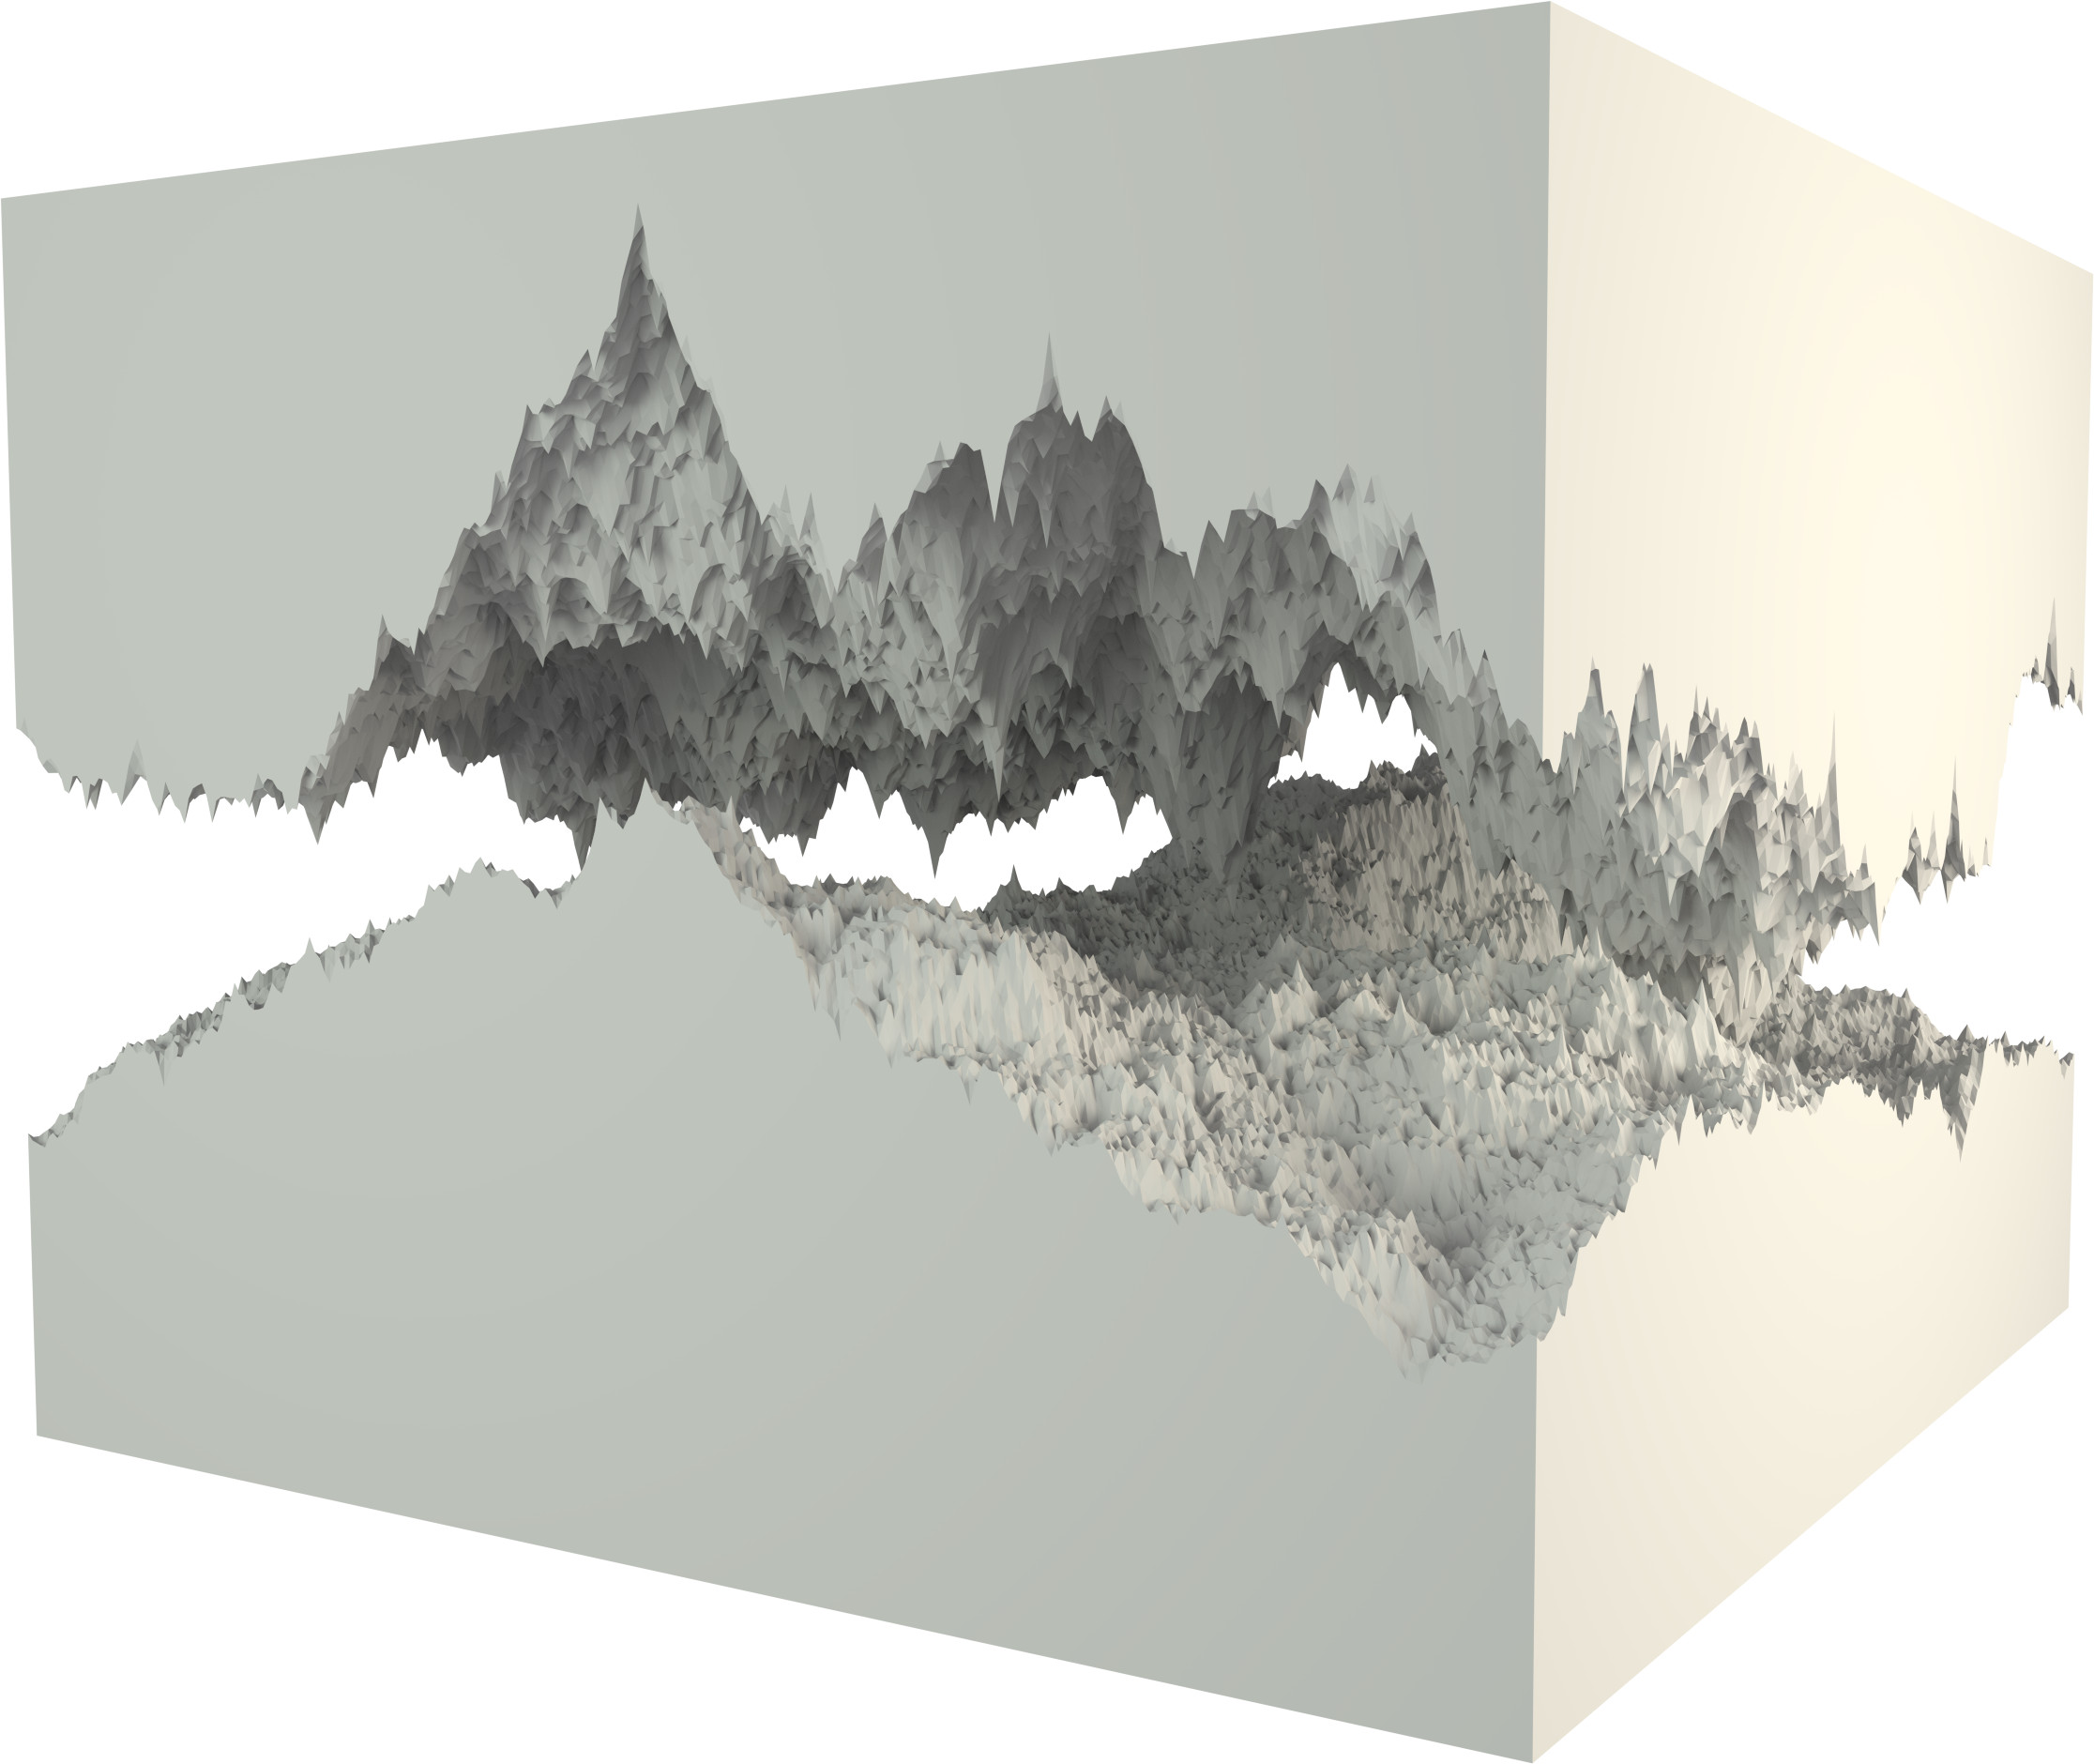
\includegraphics[width=\textwidth]{images/fracture/large_fracture05.jpg}%
    \caption{%
        A randomly generated fracture.%
    }%
\end{figure}%
\vspace{\fill}

\chapter{Introduction}
We want to study the behaviour of water trapped in nanoscale pores and fractures in silica, so need a way to generate and characterize such structures. We choose to model a fracture as two surfaces, with the volume between the surfaces as the void fraction. This makes it easier to make fractures, since we only need to create two surfaces to get a fracture. To generate realistic surfaces we could have used scans of the structures we want to simulate, but the problem with this approach is that the resulting fracture will depend a lot on how we interpret the image, and that we can not easily generate a lot of samples of surfaces. To avoid this we use fractals to describe surfaces, and use this to randomly generate surfaces and fractures that are statistically similar to real fractures. Like a lot of phenomena in nature, fractures and surfaces can be very well described by the theory of fractals\cite{mandelbrot1983fractal}, so we think that this method should give good results.

What makes a \emph{fractal} fractal, or what characterizes a fractal, does not have a rigorous definition, but in general a fractal is something that looks similar to itself at different length scales. A fractal might be \emph{identical} to itself at different length-scales \hl{(self-similar)}, or be \emph{statistically similar} to itself \hl{(statistically self-similar)}. In one dimension this looks like \todoao{Examples of 1D, scale x and y equally for self-similar, different scaling for self-affine}

Fractals and concepts similar to fractals have been discussed as early as the 17th century, but the use of fractals in natural sciences didn't really \hl{take off} before computers became \hl{readily} available and Benoit Mandelbrot gathered and developed a lot of theory on fractals in ``The Fractal Geometry of Nature''\cite{mandelbrot1983fractal}. 

\todoa{Define fractal dimension}
\todoa{More intro about fractals, some history?}
\tododone{Define fractal, define self-similarirt and similar terms}

% \todoao{change wording? copied from Fractals...}
% An \emph{affine transformation} transforms a point $\bvec x = (x_1, \dots, x_n)$ into new points $\bvec x' = (r_1x_1, \dots, r_n, x_n)$, where the scaling rations $r_1, \dots, r_n$ are \emph{not} all equal.
% 
% A bounded set $\mathcal{S}$ is \emph{self-affine} if $\mathcal{S}$ is the union of $N$ non-overlapping subsets $\mathcal{S}_1, \dots, \mathcal{S}_N$, each of which is congruent to the set $\bvec r(\mathcal{S})$ obtained from $\mathcal S$ by the affine transform defined by $\bvec r$. Here \emph{congruent} means that the set of points $\mathcal{S}$ is identical to the set of points $\bvec r(\mathcal{S})$ after possible translations and/or rotations of the set\cite{feder1988fractals}.
% 
% A set $\mathcal{S}$ is \emph{statistically self-affine} if $\mathcal{S}$ is the union of $N$ non-overlapping subsets each of which is scaled down by $\bvec r$ from the original, and is identical in all statistical respects to $\bvec r(\mathcal{S})$.

\chapter{Fractals and fractures}
\todoa{Finish fractals and fractures chapter thing}%
%
% \section{Surface area}
% \section{Distance to nearest atom}
% \begin{itemize}
%     \item Fractals
%     \item Fractional Brownian Motion
%     \item The Hurst Exponent
% \end{itemize}
To generate a fractal surface we use fractional Brownian motion \hl{(fBm)}, introduced by Mandelbrot and van Ness in 1968\cite{mandelbrot1968fractional}. Fractional Brownian motion is a generalization of Brownian motion, which is the random motion of particles suspended in a fluid, which comes from their collisions with the atoms and molecules in the fluid. 

Fractional Brownian motion is a process that generates \hl{data} that \hl{is fractal}, in the sense that it is self-similar%
. The \hl{data} generated by this process can be characterized by a parameter denoted $H$, often called the Hurst exponent. $H$ is related to the \hl{autocorrelation (define?)} of a data set, and is always a number between 0 and 1.
%It is directly related to the fractal dimension $D$ via\cite{feder1988fractals}\todoao{The Hurst exponent relates the root mean square value of the change $dy$ to the distance $x$ over which it changes}
% \begin{align*}
%     D = d - H
% \end{align*}

\hl{The Hurst exponent quantifies the relative tendency of a (time series) to either regress to the mean, or to cluster in a direction.} $H\in[0,0.5]$ indicates a \hl{time series} with long-term switching between high and low values in adjacent pairs, meaning that a single high value will probably be followed by a low value, and vice versa. $H\in[0.5,1.0]$ indicates a \hl{time series} with long-term positive autocorrelation, meaning both that a high value will probably be followed by another high value, and that the values a long time into the future will also tend to be \hl{high (increasing?)}.

Samples of \hl{fBm} with different Hurst parameters will differ in what can quantitatively be called the ``roughness'' or the ``randomness'' of the \hl{series}, as can be seen in \cref{fig:fBm_examples}, where we have plotted some samples of \hl{fBm} with different Hurst exponents.

\todo{in honor of both Harold Edwin Hurst and Ludwig Otto H\"older}

The Hurst exponent and the use of it as a means of characterizing a \hl{dataset/timeseries?} was developed \hl{in the field of hydrology}, as seen in \cite{hurst1951longterm,hurst1965longterm}, where it was used to determine the optimal dam sizing for the Nile river's, by studying the large fluctuations in the flow rate of the river, which there are extensive records of\todoco{rewrite this one-sentence paragraph}. It is denoted $H$ in honor of both Harold Hurst, who was the lead researcher in these studies, and in honor of Otto H\"older \hl{WHY H\"older?}.
%
\todobo{See \cite{mu1988steel} for ref. on fractal dimension of fractured steel surface}%
\todob{No true fractals in nature, since we need infinite resolution. $H = $ Hausdorff dimension? index-$\alpha$?}%
% \todob{Decide on which Hurst figure, and maybe resize the label box in alt. 1? (just increase fig size in plot script)}%
%
\begin{figure}[htpb]%
    \centering%
    {%
%         \newcommand{\s}{\sim}%
        \newcommand{\sa}{H $\approx$ }%
        \includesvg[width=0.8\textwidth, svgpath = ./images/Hurst/]{fbm_1d_examples_grid01}%
    }%
    \caption{%
        Samples of fractional Brownian motion (fBm) with different Hurst exponents, generated using the built-in Matlab function \mono{wfbm}, which uses uses a wavelet-based synthesis method\cite{abry1996wavelet} for generating fBm.%
    }%
    \label{fig:fBm_examples}%
\end{figure}%
% \begin{figure}[htpb]%
%     \centering%
%     \includesvg[width=1.0\textwidth, svgpath = ./images/Hurst/]{fbm_1d_examples}%
%     \caption{}%
% %     \labedl{fig:fBm_examples01}%
% \end{figure}%
%
% We will use fractional Brownian motion (fBm) to 
% We use fractional Brownian motion (fBm) to model fractures 
%
% We will use fractals both for describing, and for generating fractures.
%
% (Several methods of characterizing a fracture could be imagined (\hl{SOURCES, examples}), and we will use several of them.)        
%
% \hl{terrain == heightmap??, finn bra ord her}
%
% \orangebox{
%     \begin{itemize}
%         \item Plot 1D DMA estimate vs. synthesized 1D fBm from FracLab. Difference between with and without new $f^*$.
%         \item Plot 2D DMA estimate vs. synth. 2D fBm from FracLab? \hl{Does FracLab generated 2D?}
%         \item Plot 2D DMA est. vs. input Hurst for diamond square. Compare with and without addition and PBC.
%     \end{itemize}
% }
    \section{Hurst exponent}
One of the earliest methods for measuring the Hurst exponent is a statistical method developed by Hurst in his studies of the Nile river\cite{hurst1965longterm}\cite{hurst1951longterm}. This method is called \emph{rescaled range analysis} and was designed for use on 1-dimensional time series. The method has been generalized to higher dimensions\cite{fan2013rescaled}, but the original 1-dimensional form is shown here.
\todobo{Something about that it's hard to measure, and why.}%

\subsection{Rescaled range analysis}
\todob{Replace rescaled range with $\Delta y \propto \Delta x^H$?}
We have a 1-dimensional time series $f(t)$. The time series is first divided into intervals of length $\tau$. The average over each interval of length $\tau$ is
\begin{align*}
    \langle f \rangle_\tau = \frac{1}{\tau} \sum_{t=1}^\tau f(t).
\end{align*}
We let $F$ be the accumulated deviation from the mean
\begin{align*}
    F(t, \tau) = \sum_{t' = 1}^t \big( f(t') - \langle f \rangle_\tau \big).
\end{align*}
The difference between the maximum and minimum of the accumulated deviation from the mean is the \emph{range} R
\begin{align*}
    R(\tau) = \max_{1 \leq t \leq \tau} \big(F(t,\tau)\big) - \min_{1 \leq t \leq \tau} \big(F(t, \tau)\big).
\end{align*}
The standard deviation $S$ of the time series is estimated using
\begin{align*}
    S^2 = \frac{1}{\tau} \sum_{t=1}^\tau \big( f(t) - \langle f \rangle_\tau \big)^2.
\end{align*}
Hurst found that the observed \emph{rescaled range}, $R/S$, for many time series is described by the empirical relation\cite{feder1988fractals}
\begin{align*}
    \frac{R}{S} = \left(\frac{\tau}{2}\right)^H \sim \tau^H.
\end{align*}
We now see that we can estimate the Hurst exponent by a linear fit of the form
\begin{align*}
    \log \left(\frac{R}{S}\right) \sim H\log\tau,
\end{align*}
where we find $H$ as the slope of the linear fit.



    \section{Detrending moving average\label{sec:dma}}
\todoa{Plot of $\sigma_\text{DMA}^2$ as function of $n$ to determine $H$}
\todobo{Transition from rescaled range to surface?}
To estimate the Hurst exponent of a surface we use a method called detrending moving average (DMA) developed for 1-dimensional data by E. Alessio, A. Carbone et al.\cite{alessio2002dma}, and later generalized to higher dimensions by A. Carbone \cite{carbone2007algorithm}. 

After trying out some different methods for estimating the Hurst exponent, we ended up choosing this method both because it is \hl{easy} to understand and implement, and because it has been shown to give good results, as we will also confirm later. A more detailed comparison of different methods for estimating the Hurst exponent can be seen in\cite{shao2012comparing}, where they find that DMA and DFA (detrended fluctuation analysis) overall perform better than FA (fluctuation analysis), also being less sensitive to the choice of scaling range.%
\todo{good results, easy to implement? }%
\todoao{everything below is for 2/3 D, not always obvious}%

\subsection{Detrending moving average in 2 dimensions}
% We define a \hl{(self-affine)} surface $f(i,j)$, where $f$ is the height in the point $(i,j)$, defined in a discrete 2-dimensional domain with size $N\times N$, for $i,j = 1,\dots,N$. We divide this surface into \emph{overlapping} subsurfaces of size $n \times n$, spanning the whole surface. The \hl{lower left} corners of the surfaces are located in the points $(i,j)$ for $i,j = 1,\dots, N-n+1$ (the limits are set so that the subsurfaces stay within the domain of the surface). In each surface we find a point $(k,l) = (n-m,n-m)$ (relative to lower bottom corner of subsurface)

We define a \hl{(self-affine)} surface $f(i,j)$ of size $N,N$, with $i,j \in [1,N]$. For each point $i,j \in [1,N-n+1]$ in this surface we define a subsurface of size $n\times n$, where each subsurface consists if the points
\begin{align*}
%     (k,l) = \left([i, \dots, i+n], [j, \dots, j+n]\right)%
%     (k,l) = (i,j) + ([1\dots,n], [1,\dots,n])%
%     (k,l) = (i,j) + \left([1\dots,n], [1,\dots,n]\right) \\
    (k,l) \in \left\{ (i,j) + \left([1\dots,n], [1,\dots,n]\right)\right\}
%     (k,l) \in \left( i + [1\dots,n], j + [1,\dots,n]\right)%
\end{align*}
\begin{align*}
    \begin{pmatrix}
        k \\
        l
    \end{pmatrix}
    =
    \begin{pmatrix}
        i \\
        j
    \end{pmatrix}
    +
    \begin{pmatrix}
        1,\dots,n \\
        1,\dots,n
    \end{pmatrix}
\end{align*}%
\todoao{Decide on which vector/matrix thing}%
in the main surface. This means that the point $(i,j)$ is located in the \hl{``lower left''}\todoao{replace lower left with something smart} corner of the subsurface, that the subsurfaces overlap, and that they together span the whole main surface. The limits $i,j \in [1,N-n+1]$ are set so that all subsurfaces are \emph{inside} the main surface.

For each subsurface located at $(i,j)$ we find a point $(k_m, l_m)$ in the subsurface, which can be written as
\begin{align}
%     (k^*, l^*) = (i,j) + (n-m, n-m) %
%     (k_0, l_0) = (i,j) + (n-m, n-m) %
    (k_m, l_m) = (i,j) + (n-m, n-m), %
%     \\
%     \big(i+(n-m), j+(n-m)\big)
    \label{eq:dma_point_in_subsurface}
\end{align}
where $m$ is defined as
\begin{align*}
    &m = \lfloor n\theta \rfloor &\text{for } \theta \in [0,1).
\end{align*}
% With $\theta = 0$ the point is in the upper right corner of the subsurfaces, at $(i+n,i+n)$, for $\theta = 1/2$ the point is in the center, at $(i+n/2, i+n/2)$, and for $\theta \rightarrow 1 \rightarrow (n-1)/n$ the point is in the lower left corner, at $(i,j)$.
The parameter $\theta$ controls the position of this point inside the subsurface, and we have three extreme cases, listed below, and illustrated in \cref{fig:DMA_theta}.%
%
\begin{description}[%
    labelindent=\oldparindent,%
%     leftmargin=12em%
    leftmargin=2.0\oldparindent%
]%
    \item[$\bm{\theta = 0}$:] the point $(k_m, l_m)$ is in the upper right corner of the subsurface, \\at ${(k_m, l_m) = (i+n,i+n)}$
    \item[$\bm{\theta = 1/2}$:] the point $(k_m, l_m)$ is in the center of the subsurface, \\at ${(k_m, l_m) = (i+n/2, i+n/2)}$
    \item[$\bm{\theta \rightarrow 1 \rightarrow (n-1)/n}$:] the point $(k_m, l_m)$ is in the lower left corner of the subsurface, at ${(k_m, l_m) = (i,j)}$
\end{description}%
% \begin{itemize}[label={}]
%     \item $\bm{\theta = 0:}$ the point $(k_m, l_m)$ is in the upper right corner of the subsurface, at $(i+n,j+n)$
%     \item $\bm{\theta = 1/2:}$ the point $(k_m, l_m)$ is in the center, at $(i+n/2, j+n/2)$
%     \item $\bm{\theta \rightarrow 1 \rightarrow (n-1)/n:}$ the point $(k_m, l_m)$ is in the lower left corner, at $(i,j)$
% \end{itemize}
%
\begin{figure}[htpb]%
    \centering%
    \vspace{1em}% Add some space so the figure isn't as close to the content above
    \begin{subfigure}[b]{0.25\textwidth}%
        \includesvg[width=\textwidth, svgpath=./images/Hurst/]{2DDMA_theta04_a}%
%         \caption{Illustration of how to divide a convex hexahedron into five tetraheda.}%
        \caption{$\theta = 0$}%
        \label{fig:DMA_theta_a}%
    \end{subfigure}%
    \hspace{0.1\textwidth}%
    \begin{subfigure}[b]{0.25\textwidth}%
        \includesvg[width=\textwidth, svgpath=./images/Hurst/]{2DDMA_theta04_b}%
%         \caption{A random fracture made from two periodic heightmaps.}%
        \caption{$\theta = 1/2$}%
        \label{fig:DMA_theta_b}%
    \end{subfigure}%
    \hspace{0.1\textwidth}%
    \begin{subfigure}[b]{0.25\textwidth}%
        \includesvg[width=\textwidth, svgpath=./images/Hurst/]{2DDMA_theta04_c}%
%         \caption{A random fracture made from two periodic heightmaps.}%
%         \caption{$\theta \rightarrow 1$ \\ ($\theta = (n-1)/n$)}%
%         \caption{$\theta \rightarrow 1$}%
        \caption{$\theta = (n-1)/n$}%
        \label{fig:DMA_theta_c}%
    \end{subfigure}%
        \caption{%
        Illustration of three extreme cases for the parameter $\theta$ in \hl{2/3} dimensions. The dots are points where the main surface is defined, the red star is the point $(k_m,j_m)$, and the black square marks the subsurface, and the points averaged over to calculate $\bar {f_n}(i,j)$ in \cref{eq:carbone_average}. The illustrations use $n = 3$.%
        \label{fig:DMA_theta}%
    }%
\end{figure}%

We find the average $\bar {f_n}$ of each subsurface \hl{using}
\begin{align}
    \bar {f_n}(i,j) = \frac{1}{n^2} \sum_{k = i}^{i+n} \sum_{l = j}^{j+n} f(k,l),
    \label{eq:carbone_average}
\end{align}
and we define the \emph{generalized variance}, $\sigma_\text{DMA}^2$, as \hl{the sum of the squared differences between} the value in the point $f(k_m,l_m)$ minus the average $\bar {f_n}(i,j)$, for each subsurface. This can be written as
\begin{align}
    \sigma_\text{DMA}^2 
%     &= \frac{1}{(N-n)^2}\sum_{i=n-m}^{N-m} ~ \sum_{j=n-m}^{N-m} 
%     \big(
%         f(i,j) - \tilde f_n(i,j)
%     \big)^2,% \label{eq:dma_variance}
%     \\
    &= \frac{1}{(N-n)^2}\sum_{i=1}^{N-n+1} ~ \sum_{j=1}^{N-n+1} 
    \big(
        f(k_m,j_m) - \bar f_n(i,j)
    \big)^2%
%     \qquad\text{for } k_m, j_m \text{as in \cref{eq:dma_point_in_subsurface}}%
    \nonumber\\%
    &= \frac{1}{(N-n)^2}\sum_{i=1}^{N-n+1} ~ \sum_{j=1}^{N-n+1} 
    \big(
        f(i+n-m,j+n-m) - \bar f_n(i,j)
    \big)^2.
    \label{eq:dma_variance}
\end{align}

It can be shown that this generalized variance has a power-law dependence on $n$ \cite{alessio2002dma,carbone2007algorithm}, which goes as
\begin{align*}
    \sigma_\text{DMA}^2 \sim \left(2n^2\right)^H.
\end{align*}
We can use this dependence to estimate the Hurst exponent $H$, by calculating $\sigma_\text{DMA}^2$ for different sizes of the subsurfaces, $n$. We estimate $H$ by a linear fit of $\log \left(\sigma_\text{DMA}\right)^2$ against $\log \left(2n^2 \right)$, where $H$ is the slope of this fit.

In the paper by Anna Carbone that generalizes DMA to higher dimensions\cite{carbone2007algorithm} they use different parameters for each spatial dimension $d$, $\bvec\theta = \theta_1, \dots, \theta_d$ and $\bvec{n} = n_1, \dots, n_d$, but for simplicity and to avoid \hl{strange/spurious?} results, we use $\theta_1 = \theta_2 = \theta$ and $n_1 = n_2 = n$.

A modification of the method mentioned is replacing $\bar f_n(i,j)$ in \cref{eq:dma_variance} with\todoao{check this equation}
\begin{align*}
    \bar {f_n}^*(i,j) = (1-\alpha) f_n(i,j) + \alpha \bar {f_n}(i-1,j-1),
\end{align*}
where
\[
    \alpha = n^2/(n+1)^2,
\]
and $\tilde f_n(i,j)$ has the same form as before (see \cref{eq:carbone_average}). To use this modification we also have to change the limits in \cref{eq:dma_variance} from ${i,j\in [1,N-n+1]}$ to $i,j\in [2,N-n+1]$. This modification has been shown to give better results for small systems\cite{carbone2007algorithm}\todo{why?}, and since we are usually generating surfaces with a \hl{resolution/$N$ of 100-200}, we use this modified method in our implementation of the method. \todo{maybe implement both methods?}

\todob{The method is implemented in Matlab/Octave}

\subsection{The performance of detrending moving average}
\todoa{Read through DMA performance, make some conclusions from plot}
To verify that the method we used for estimating the Hurst exponent worked as intended, and gave good results, we ran a series of tests using synthetic \hl{(1D)} time series and \hl{(2D)} surfaces \hl{of fractional Brownian motion} with a known Hurst exponent. When doing these tests we soon realized that a big problem with synthesizing time series and surfaces with a given Hurst exponent is that it's both hard to accurately measure the exponent, and it's hard to synthesize data with a given exponent. \hl{This means that when testing methods for analysing and synthesizing signals, you never know if it's you measuring method, or your synthesizing method that is causing problems if things aren't working as intended.}

To test the \hl{DMA method} we synthesized data with a given Hurst exponent using 4 different \hl{methods/programs}, and measured the exponent using the detrending moving average method for each of these methods. 

For synthesizing 1D data we used the built-in Matlab-function \hl{cite matlab?} \Verb!wfbm! which uses a wavelet-based synthesis method described by Abry and Sellan \cite{abry1996wavelet}, and two methods from the Matlab-toolbox FracLab\cite{fraclab_toolbox}, \Verb!fbmwoodchan! which uses a method proposed by Wood and Chan in \cite{wood1994simulation}, and \Verb!fbmlevinson! which uses Cholesky/Levinson factorization from \cite{levinson1947wiener}. 

There are many methods and algorithms for generating \hl{2D/3D/surfaces} data with a given Hurst exponent, but we had problems finding working implementations of any of them. We will later implement a midpoint displacement method for this (see \cref{chap:generating_surfaces,subsec:SRA_implementation}), but having external reference is very useful, so we used a function from FracLab called \Verb!synth2!, which, according to the documentation of the function:%
\begin{quote}
    \textit{Generates a 2D Fractional Brownian Motion (fBm) using an incremental Fourier Method for processes with stationary increments of order (0,1) and (1,0).}
\end{quote}\todobo{No sources are given in FracLab documentation...}
We will later also test our own implementation of a method for generating \hl{2d/3d} data against \hl{DMA}.
% ``Generates a 2D Fractional Brownian Motion (fBm) using an incremental Fourier Method for processes with stationary increments of order (0,1) and (1,0)''.

See \cref{fig:dma_performace} for a plot of Hurst exponent measured using \hl{DMA} as a function of the exponent used as input for the four different methods for generating synthetic data above, for three different values of the parameter $\theta$.

From \cref{fig:dma_performace} we conclude that $\theta = 0.0$ seems to give the best and most consistent results, as also noted by Gao-Feng Gu and Wei-Xing Zhou in\cite{gu2010detrending}, where they further develop the \hl{DMA} method to analyse multifractals. \hl{We would liked to have more 2D data references.}%
\todob{Fix newcommand stuff in \cref{fig:dma_performace}, and maybe legend texts (can remove stuff now that we know have smaller text in figures)}
%
\begin{figure}[htpb]%
    \centering%
    {
        \newcommand{\f}{\footnotesize}%
        \newcommand{\x}{\text}%
        \newcommand{\thislabelaaaaaa}{{\f $H_\x{in}=H_\x{out}$}}%
        \includesvg[width=1.0\textwidth, svgpath=./images/diamond_square_Hurst/test_HDDMA/]{fig03}%
    }
%     \caption[
%         Plot of the Hurst exponent as estimated by the detrending moving average method, used on data from four different synthetic signals, against the exponent used as input when generating the signals, and for three different values of the parameter $\theta$ used in \hl{DMA}. All methods except synth2 generate 1-dimensional signals, while synth2 generates a 2-dimensional signal. \hl{FINISH CAPTION}. %
%     ]{%
%         Plot of the Hurst exponent as estimated by the detrending moving average method, used on data from four different synthetic signals, against the exponent used as input when generating the signals, and for three different values of the parameter $\theta$ used in \hl{DMA}. All methods except \Verb!synth2! generate 1-dimensional signals, while \mono{synth2} generates a 2-dimensional signal. \hl{FINISH CAPTION}. %
%         \label{fig:dma_performace}%
%     }%
    \caption{%
        Plot of the Hurst exponent against the exponent used as input when generating the signals, as estimated by the detrending moving average method, used on data from four different synthetic signals, and for three different values of the parameter $\theta$ used in \hl{DMA}. For the 1d methods we have averaged over 1000 samples for each point, and for \mono{synth2} we have averaged over 100 samples, for input Hurst exponents between 0.05 and 0.95 in steps of 0.1. All methods except \mono{synth2} generate 1-dimensional signals, while \mono{synth2} generates a 2-dimensional signal. \hl{FINISH CAPTION}. %
        \label{fig:dma_performace}%
    }%
\end{figure}%

\orangebox{
    \begin{itemize}
        \item 1D: Plot of H from DMA vs. input H for wfbm (Matlab built in), and perhaps a FracLab variant?
        \item 1D: Plot of H from DMA vs. H from FracLab measure method?
        \item 2D: Plot of H from DMA vs. input DiamondSquare H and vs. synth2? (this could fit better in diamondsquare part).
    \end{itemize}
}

    \chapter{Generating surfaces}
\hl{Stuff to define?}
\begin{itemize}
    \item fBm surfaces
    \item Hurst exponent
    \item Gaussian random variable ?
    \item non-stationary
    \item self-similar
    \item isotropic
    \item lacunarity
\end{itemize}

Introduction?
% When generating random surfaces we want to be able to control the properties like the Hurst exponent (\hl{etc.?}) of the surface.

To generate our random surfaces we use an iterative midpoint displacement method usually called successive random additions \hl{(SRA)}. The method is based on a method proposed by Fourner in 1982\cite{fournier1982computer}, but with some modifications suggested by Voss\cite{voss1985random, voss1988fractals}. The method has further been discussed by Saupe\cite{saupe1988algorithms}, amongst others. We choose this method mainly because it's possible to generate periodic surfaces with it, because it generates very good approximations to fBm surfaces\cite{zhou2005comparison}, and because the Hurst exponent of the generated surfaces is easy to control. The method is also easy to understand, easy to implement, and generates surfaces with high resolution very fast. The method is widely used in scientific applications\hl{cite??} because of these properties, and is also used for generating surfaces in computer graphics, since the surfaces look very realistic \hl{with only some minor artefacts?? (high, narrow peaks)}.

\section{Midpoint displacement methods (in 1 dimension)}
\todo[inline]{The most basic method we used is a very basic but widely used method, which has many variations and names. The most common names are ``the diamond-square algorithm''\hl{cite}, ``the midpoint displacement method''\hl{cite}, ``plasma fractal'' and ``cloud fractal''.}

The method we use to generate random surfaces is very similar to the standard midpoint displacement method, which in 1 dimension goes as follows. See \cref{fig:midpoint01} for a visual presentation.
%
\begin{enumerate}
    \item Give the values at the endpoints of the interval, $y_0$ and $y_n$, random values from a Gaussian random variable with mean $\mu = 0$ and variance $\sigma_0^2$. This initial standard deviation $\sigma_0$ can be chosen freely.
    \item Generate the value in the center of the interval, $y_{n/2}$, by averaging over the two endpoints and adding a Gaussian random number with mean $\mu = 0$ and a \emph{reduced} variance
    \begin{align}
         \sigma_1^2 = \left(1/2\right)^{2H}\sigma_0^2, \label{eq:midpoint_sigma_first}
    \end{align}
    where $H$ is the wanted Hurst exponent.
    \item Continue generating the values in the center of each sub-interval until you reach the desired number of points, while reducing the variance of the random number by a factor $\frac{1}{2}$ each iteration\todo{Why 1/2? (needed to create good approx. to fBm, see \cite{voss1985random})}. For iteration $i$ we have
    \begin{align}
        \sigma_i^2 = \left(1/2\right)^{i2H}\sigma_0^2. \label{eq:midpoint_sigma_general}
    \end{align}
\end{enumerate}
%
\begin{figure}[htpb]%
    \centering%
    \includesvg[width=0.5\textwidth, svgpath=./images/diamond_square/]{random_midpoint_displacement_regular02}%
    \caption{%
        \hl{Illustration of the midpoint displacement method in 1 dimension. We increase the number of points from 2 to 9 using 3 iterations.}%
        \label{fig:midpoint01}%
    }%
\end{figure}%

This method generates a \hl{1-dimensional line}, with a Hurst exponent \hl{close} to the input $H$\todo{how close?}. But since we only add random numbers to the new values, the result is non-stationary for $H \neq 0.5$\cite{voss1985random}\hl{, and it is neither self-similar or isotropic, as noted by Mandelbrot}\cite{mandelbrot1982comment}. To mitigate this we implement the addition suggested by Voss\cite{voss1985random}, which consists of adding a random number to \emph{all} points in each iteration, both the new and old. Voss called this modified method \emph{successive random additions}.

\section{Successive random additions in 2 dimensions}
As mentioned \st{before}, the method called \emph{successive random additions} is a modification of the regular midpoint displacement method first described by Richard F. Voss\cite{voss1985random}, where we add random numbers to \emph{all} points in each iteration, compared to just the \emph{new} points in the regular midpoint displacement method. This modification means that we can replace the factor $(1/2)$ in \cref{eq:midpoint_sigma_first,eq:midpoint_sigma_general} with a general factor $r$\todo{why? (something about distance between points)}, and we get
\begin{align*}
    \sigma_i^2 = r^{2H}\sigma^2_{i-1}.
\end{align*}
\hl{$r$ controls the lacunarity/roughness, $H$ independent of $r$}

% \subsection{(on an infinite grid) in 2 dimensions}
\subsection{On an infinite grid}
Voss has geneneralized the the method of successive random additions to higher dimensions\cite{voss1985random}, and this generalized form is the algorithm we use when generating fractures. We generate surfaces in the form of heightmaps, meaning a 2-dimensional grid of points ({$x,y$}), with a value for the height in each point \hl{($z(x,y) = z_{x,y}$)} which is generated by the algorithm.

The central part of the algorithm consists of two steps often called the \emph{diamond-step} and the \emph{square-step}. We start with a simple case of an infinite grid of evenly spaced points, all with known $z$-values. The two steps are as follows:
\begin{description}
    \item[The \emph{square-step}:] The grid can be divided into small squares consisting of four points in each square, as in the leftmost square in \cref{fig:simple_square_step}. We generate the $z$-value in the center of each of these squares by averaging the $z$-values of the four corners of each square, as indicated by the red dots and arrows in \cref{fig:simple_square_step}. Then add a random Gaussian number with mean $\mu = 0$ and variance $\sigma_i^2 = \sigma_{i-1}^2r^{2H}$ to all new and old points, where $\sigma_{i-1}^2$ is the variance used in the last step of the algorithm.
    \label{enum:test}
    
    \item[The \emph{diamond-step}:] After the square-step the grid can be divided into smaller squares that are tilded by 45 degrees, as in the leftmost square in \cref{fig:simple_diamond_step}. We generate the $z$-values in the center of each square by averaging the $z$-values of the four corners of each square, as indicated by the red dots and arrows in \cref{fig:simple_diamond_step}. We then add a random Gaussian number with mean $\mu = 0$ and variance $\sigma_{i+1}^2 = \sigma_i^2r^{2H}$, to all new and old points. 
\end{description}
See \cref{fig:diamond_square_applied} for an illustration of the algorithm applied once on a larger grid. 

\begin{figure}[htpb]%
\centering%
%
\setlength{\myfigwidth}{0.5\textwidth}%
\setlength{\mycaptionwidth}{0.3\textwidth}%
%
% \parbox[c][2cm][c]{\myfigwidth}{
%     \includesvg[width=\myfigwidth, svgpath = images/diamond_square/]{simple_square_step_solarized08}
% }
% \parbox[c][2cm][c]{\mycaptionwidth}{
%     \subcaption{Square-step}
%     \label{fig:simple_square_step}
% }
%
% \begin{minipage}[c][2cm][c]{\myfigwidth}
%     \includesvg[height=2cm, svgpath = images/diamond_square/]{simple_square_step_solarized08}
% \end{minipage}
% \begin{minipage}[c][2cm][c]{\mycaptionwidth}
%     \subcaption{Square-step}
%     \label{fig:simple_square_step}
% \end{minipage}
%
\begin{minipage}[c]{\myfigwidth}%
    \includesvg[width=\textwidth, svgpath = images/diamond_square/]{simple_square_step_solarized08}%
\end{minipage}%
\begin{minipage}[c]{\mycaptionwidth}%
    \subcaption{Square-step}%
    \label{fig:simple_square_step}%
\end{minipage}%
\\%
\vspace{2mm}%
\begin{minipage}[c]{\myfigwidth}%
    \includesvg[width=\textwidth, svgpath = images/diamond_square/]{simple_diamond_step_solarized05}%
\end{minipage}%
\begin{minipage}[c]{\mycaptionwidth}%
    \subcaption{Diamond-step}%
    \label{fig:simple_diamond_step}%
\end{minipage}%
%
\caption{Illustration of the two steps used in the diamond square algorithm for generating random surfaces. The grey points are old points, the black points are new points, and the red points are the points used in the calcuation of the averages when generating the new points.}%
\label{fig:diamond_square_steps}%
\end{figure}%

We see that by first applying the square-step and then applying the diamond-step, we add one point in between each point in each direction, almost doubling the resolution of the grid. In general we go from $n$ to $n + (n-1)$ points in each direction. By applying the algorithm several times we get \todo{replace $n$ with $N$ and $i$ with $n$?}
\begin{align}
    n_1 &= n_0 + (n_0-1) = 2n - 1 \nonumber\\
    n_2 &= 2n_1 - 1 = 4n_0 - 3 \nonumber\\
    n_3 &= 2n_2 - 1 = 9n_0 - 7 \nonumber\\
    &\vdotswithin{=} \nonumber\\
%     &\shortvdotswithin{=}
    n_i &= 2^i(n_0-1) + 1, \label{eq:diamond_step_resolution}
\end{align}
where $i$ is the number of times we have applied the algorithm. This means that using the diamond-square algorithm we can go from any resolution $n_0$ to all resolutions satisfying $n_i = 2^i(n_0 - 1) + 1$.
%
\begin{figure}[htpb]%
    \centering%
    \includesvg[width=0.7\textwidth, svgpath = images/diamond_square/]{increase_resolution_solarized_starssquares03}%
    \caption{%
        The diamond-square algorithm applied once on a grid of $3\times 3$ points, increasing the number of points from 9 to 25. The orange square points are generated by the square-step (see \cref{fig:simple_square_step}), and the blue star-shaped points by the diamond-step (see \cref{fig:simple_diamond_step}).%
    }%
    \label{fig:diamond_square_applied}%
\end{figure}%

% \subsection{Successive random additions on a finite grid (in 2 dimensions)}
\subsection{On a finite grid}
Since we are using computers to generate our surfaces, which have limited memory, we can't use infinite grids. This means we get some special cases that needs to be taken care of when generating points near the edges of the grid.\todo{transition to below}

For the square step we generate one new point in the center each square formed by the grid from the previous iteration, and in general we generate the $z$-values in the points
\begin{align}
    &\left(x_{i+1/2}, y_{j+1/2}\right) &0\leq i,j < n, \label{eq:square_step_limits}
\end{align}
where $(x_i,x_j)$ are the points in the grid after the last iteration. In general the averages we calculate for the new points can be written as\todo{make this equation nicer}
% \begin{align}
%     (x_{i+1/2}, y_{j+1/2}) 
%     &= \frac{1}{4}\big(
%         (x_i, y_j) + (x_{i+1}, y_j)\nonumber\\
%         &+ (x_i, y_{j+1}) + (x_{i+1}, y_{j+1})
%     \big)
%     &0\leq i,j < n.
%     \label{eq:square_step}
% \end{align}
\begin{align}
    (x_{i+1/2}, y_{j+1/2}) 
    = \frac{1}{4}\big[
        (x_i, y_j) + (x_{i+1}, y_j)
        &+ (x_i, y_{j+1}) + (x_{i+1}, y_{j+1})
    \big],
    \label{eq:square_step}
\end{align}
using the limits in \cref{eq:square_step_limits}. We see that the square-step only uses points inside the grid, which means that we don't have to modify it when going to a finite grid.

For the diamond-step we generate the values in the points

\begin{align}
    &(x_{i+1/2}, y_j) &\text{for } 0\leq i<n \text{ and } 0\leq j \leq n& \label{eq:diamond_step_limits01}\\
    &(x_i, y_{j+1/2}) &\text{for } 0\leq i\leq n \text{ and } 0\leq j < n&. \label{eq:diamond_step_limits02}
\end{align}
In general the averages we calculate for the new points can be written as\todo{make these equations nicer}
% \begin{align}
%     (x_{i+1/2}, y_j) 
%     &= 
%     \frac{1}{4}\big(
%         (x_i, y_j) + (x_{i+1}, y_j) + (x_{i+1/2}, y_{j-1/2}) + (x_{i+1/2}, y_{j+1/2})
%     \big) \label{eq:diamond_step01}\\
%     (x_i, y_{j+1/2}) 
%     &= 
%     \frac{1}{4}\big(
%         (x_i, y_j) + (x_i, y_{j+1}) + (x_{i-1/2}, y_{j+1/2}) + (x_{i+1/2}, y_{j+1/2})
%     \big). \label{eq:diamond_step02}
% \end{align}
\begin{align}
    (x_{i+1/2}, y_j) 
    &= 
    \frac{1}{4}\big[
        (x_i, y_j) + (x_{i+1}, y_j) \nonumber\\
        &+ (x_{i+1/2}, y_{j-1/2}) + (x_{i+1/2}, y_{j+1/2})
    \big]
    \label{eq:diamond_step01}\\
    (x_i, y_{j+1/2}) 
    &= 
    \frac{1}{4}\big[
        (x_i, y_j) + (x_i, y_{j+1}) \nonumber\\
        &+ (x_{i-1/2}, y_{j+1/2}) + (x_{i+1/2}, y_{j+1/2})
    \big],
    \label{eq:diamond_step02}
\end{align}
using the limits in \cref{eq:diamond_step_limits01,eq:diamond_step_limits02}. We now see that when generating points near the edges using the diamond-step, specifically when generating the points $(x_{i+1/2}, y_j)$ for $j \in \{0, n\}$ and $(x_i, y_{j+1/2})$ for $i = \{0, n\}$, we need to average over points that lie outside the grid. There are two possible solutions, depending on the surface we are generating. If generating a periodic surface, the solution is to wrap around the edges using periodic boundary conditions, and find the point we need on the opposite side of the grid. For example (using $i = j = 0$)
\begin{align*}
    (x_{1/2}, y_{-1/2}) = (x_{1/2}, y_{n-1/2}).
\end{align*}
If generating a non-periodic grid we simply ignore the points that lie outside the grid when calculating the averages, and just use the \hl{three/3} other points.

% \subsection{Implementing successive random additions (on a finite grid in 2 dimensions)}
\subsection{Implementation}
In our implementation we generate a surface on a finite grid of size $N\times N$, starting with only the $z$-values in the four corners defined, giving a resolution $n_0 = 2$. As shown in \cref{eq:diamond_step_resolution} the algorithm can go from any resolution $n_0$ to any resolution \hl{of the form} $n_p = 2^p(n_0-1) + 1$ by applying the algorithm $p$ times, which means that our implementation can generate surfaces with resolutions
\begin{align*}
    N &= 2^p(2-1) + 1 = 2^p + 1,
\end{align*}
where $p$ is any positive integer.

We implement generation of both periodic and non-periodic surfaces using using \crefrange{eq:square_step_limits}{eq:diamond_step02}, while skipping points outside the grid for non-periodic surfaces, and wrapping around the edges using periodic boundary conditions when generating periodic surfaces.

To ensure that the periodic surfaces actually turn out periodic we start with all four corners having the same value. We also let the right and bottom edge be equivalent to the left and top edge, respectively, which effectively means that all four corners should always have the same $z$-value. To ensure that the opposite edges stay equal to each other we never generate any points on the right and bottom edge, but just copy the $z$-values from the opposite \hl{corresponding} edge after the diamond-step.

This leaves us with the following algorithm for generating a surface which approximates a 2-dimensional fractional Brownian motion with Hurst exponent $H$
\begin{enumerate}
    % \itemsep1pt \parskip0pt \parsep0pt
    \renewcommand{\labelitemii}{$\bullet$}
    
    \item Allocate a grid of size $N\times N$, where $N = 2^p + 1$, and $p$ is any positive integer. \hl{This grid will store the $z$-values, or the height of the surface, in each grid point $(x,y)$.}

    \item Initialize the $z$-values of the corners of the grid by drawing random numbers from a Gaussian distribution with mean $\mu = 0$ and variance $\sigma_0$. The initial variance can be chosen freely. \hl{The initial resolution is now $n_0\times n_0$, with $n = 2$}.
    \begin{itemize}
        \item If generating a periodic surface, give all four corners the same $z$-value.
    \end{itemize}
    
    \item Apply the square-step using \cref{eq:square_step_limits,eq:square_step}. Add a random Gaussian number with mean $\mu = 0$ and variance $\sigma_i = \sigma_{i-1}^2r^{2H}$ to all new and old points.
    \label{enum:square_step}

    \item Apply the diamond-step using \crefrange{eq:diamond_step01}{eq:diamond_step02}. Add a random Gaussian number with mean $\mu = 0$ and variance $\sigma_{i+1} = \sigma_i^2r^{2H}$ to all new and old points.
    \label{enum:diamond_step}
    
    \begin{itemize}
        \item If generating a periodic surface, skip generating $z$-values for points on the right and bottom edge using the diamond-step, and instead copy the values from the opposite edges after the diamond-step.
    \end{itemize}
    
    \item Repeat step \ref{enum:square_step} and \ref{enum:diamond_step} $p$ times until you reach the desired resolution of $N\times N$, where $N = 2^p + 1$. For step $i$ the variance of the random Gaussian numbers is
    \begin{align*}
        \sigma_i^2 = \sigma_0^2(r^i)^{2H}.
    \end{align*}
\end{enumerate}

See \cref{fig:diamond_square_surface} for a surface generated by the algorithm.
%
% \begin{figure}[htpb]%
%     \centering%
%     \includesvg[width=0.7\textwidth, svgpath=./images/diamond_square/surface_example/]{surface_labels}%
%     \caption{%
%         Caption.%
%         \label{fig:diamond_square_surface}%
%     }%
% \end{figure}%
\begin{figure}[htpb]%
    \centering%
    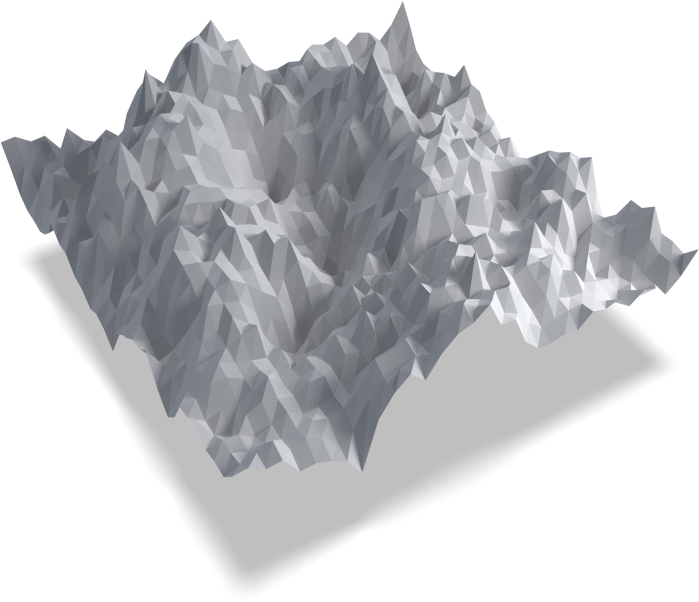
\includegraphics[width=0.5\textwidth]{./images/diamond_square/surface_blender/surface_composite01_cropped.png}%
    \caption{%
        Caption.%
        \label{fig:diamond_square_surface}%
    }%
\end{figure}%

\orangebox{
{\bf Notes:}
\begin{itemize}
    \item Implementation (in Matlab/C++)?
    \item periodic and non-periodic
    \item Mention that DS can be used to increase resolution of any surface
    \item Can increase resolution of generated surface, if we know the seed
\end{itemize}

{\bf Stuff to define:}
\begin{itemize}
    \item Periodic/non-periodic
    \item Lacunarity
\end{itemize}
}

\subsection{Testing the method}
%
\begin{figure}[htpb]%
    \centering%
    {
        \newcommand{\f}{\footnotesize}%
        \newcommand{\x}{\text}%
        \newcommand{\hh}{{\f $H_\x{in}=H_\x{out}$}}%
        \includesvg[width=0.7\textwidth, svgpath=./images/diamond_square_Hurst/test_diamondSquare/]{fig}%
    }
    \caption{%
        Diamond square accuracy? Measured using DMA. The dashed grey line indicates a measured Hurst exponent of 0.75, the solid grey line a measured exponent exactly equal to the input exponent. The green lines are surfaces created using periodic boundary conditions (PBC), the red lines using non-periodic boundaries, the dashed lines using successive random additions (SRA), and the solid lines using the regular midpoint displacement method (MDM). \hl{FINISH CAPTION}. %
%         \label{fig:cell_lists}%
    }%
\end{figure}%

    \section{Generating fractures from surfaces\label{sec:generating_fractures}}
To generate a realistic fracture we use the method of successive random additions described in \cref{chap:generating_surfaces,subsec:SRA_implementation} to generate random surfaces with a known Hurst exponent. We then displace the surfaces in the $z$-direction, so one is above the other, and let the space between the surfaces be the void\footnote{Since we are using periodic systems, we could also have let the space outside the surfaces be the fracture and get the same result. But for easier visualization and understanding we use the volume between the surfaces.}.

In practice we make a fractured silica structure using the following procedure
\begin{itemize}
    \item Prepare a slab of amorphous SiO$_2$.
    \item Generate two surfaces.
    \item Rescale the $(x,y)$-positions of surfaces so they span the molecular system.
    \item Rescale the $z$-values of the surfaces so all points are inside the system.
    \item Remove all atoms between the upper and lower surface.
\end{itemize}

The biggest problem with this procedure is removing the atoms between two surfaces. But since all points in both surfaces lie on a regular grid in the $x$-$y$-plane, there is a simple way of dividing the volume between the surfaces into tetrahedra. And checking if a point is inside a tetrahedra is a geometrical exercize that can be solved programmatically. If the two surfaces are not intersecting, we can divide the volume between them into convex hexahedra spanned out by the points
% \begin{align*}
%     (x^1_{i}, y^1_{i}), (x^1_{i+1}, y^1_{i}), (x^1_{i}, y^1_{i+1}), (x^1_{i+1}, y^1_{i+1}), \\
%     (x^2_{i}, y^2_{i}), (x^2_{i+1}, y^2_{i}), (x^2_{i}, y^2_{i+1}), (x^2_{i+1}, y^2_{i+1}),
% \end{align*}
\begin{align*}
    z(i,j)&, & &z(i+1,j),& & &z(i,j+1)&, &\text{and}& & &z(i+1,j+1)& & &\text{for} & &i,j \in [0,N)
\end{align*}
in the two surfaces (four points in each surface). We then divide each convex hexahedra into five tetraheda, as illustrated in \cref{fig:hex_to_tetra}, giving a total of $5(N-1)^2$ tetrahedra spanning the total volume between the two surfaces.
%
% We do this by utilizing the fact that the points in each heighmap lie on a regular grid in the $x$-$y$-plane. This means that we can divide the volume into tetrahedra, . If the two heightmaps are not intersecting, we see that we can divide the volume between them into convex hexahedra, one for each set of points
% ($x_{i}, y_{i}$), ($x_{i}, y_{i+1}$), ($x_{i+1}, y_{i}$), and ($x_{i+1}, y_{i+1}$) 
% % $(x_i, y_i)$  $(x_i, y_{i+1})$ $(x_{i+1}, y_i)$ $(x_{i+1}, y_{i+1})$
% in the $x$-$y$-grid. Each of these hexahedra can then be divided into five tetrahedra, as illustrated in \cref{fig:hex_to_tetra}.
%
% \begin{figure}[htpb]%
%     \centering%
%     
\includegraphics[width=0.4\textwidth]{images/fracture/hexahedron_to_tetrahedra.png}%
%     \caption{%
%         Illustration of how to divide a hexahedron into five tetraheda.%
%         \label{fig:hex_to_tetra}%
%     }%
% \end{figure}%
% %
% \begin{figure}[htpb]%
%     \centering%
%     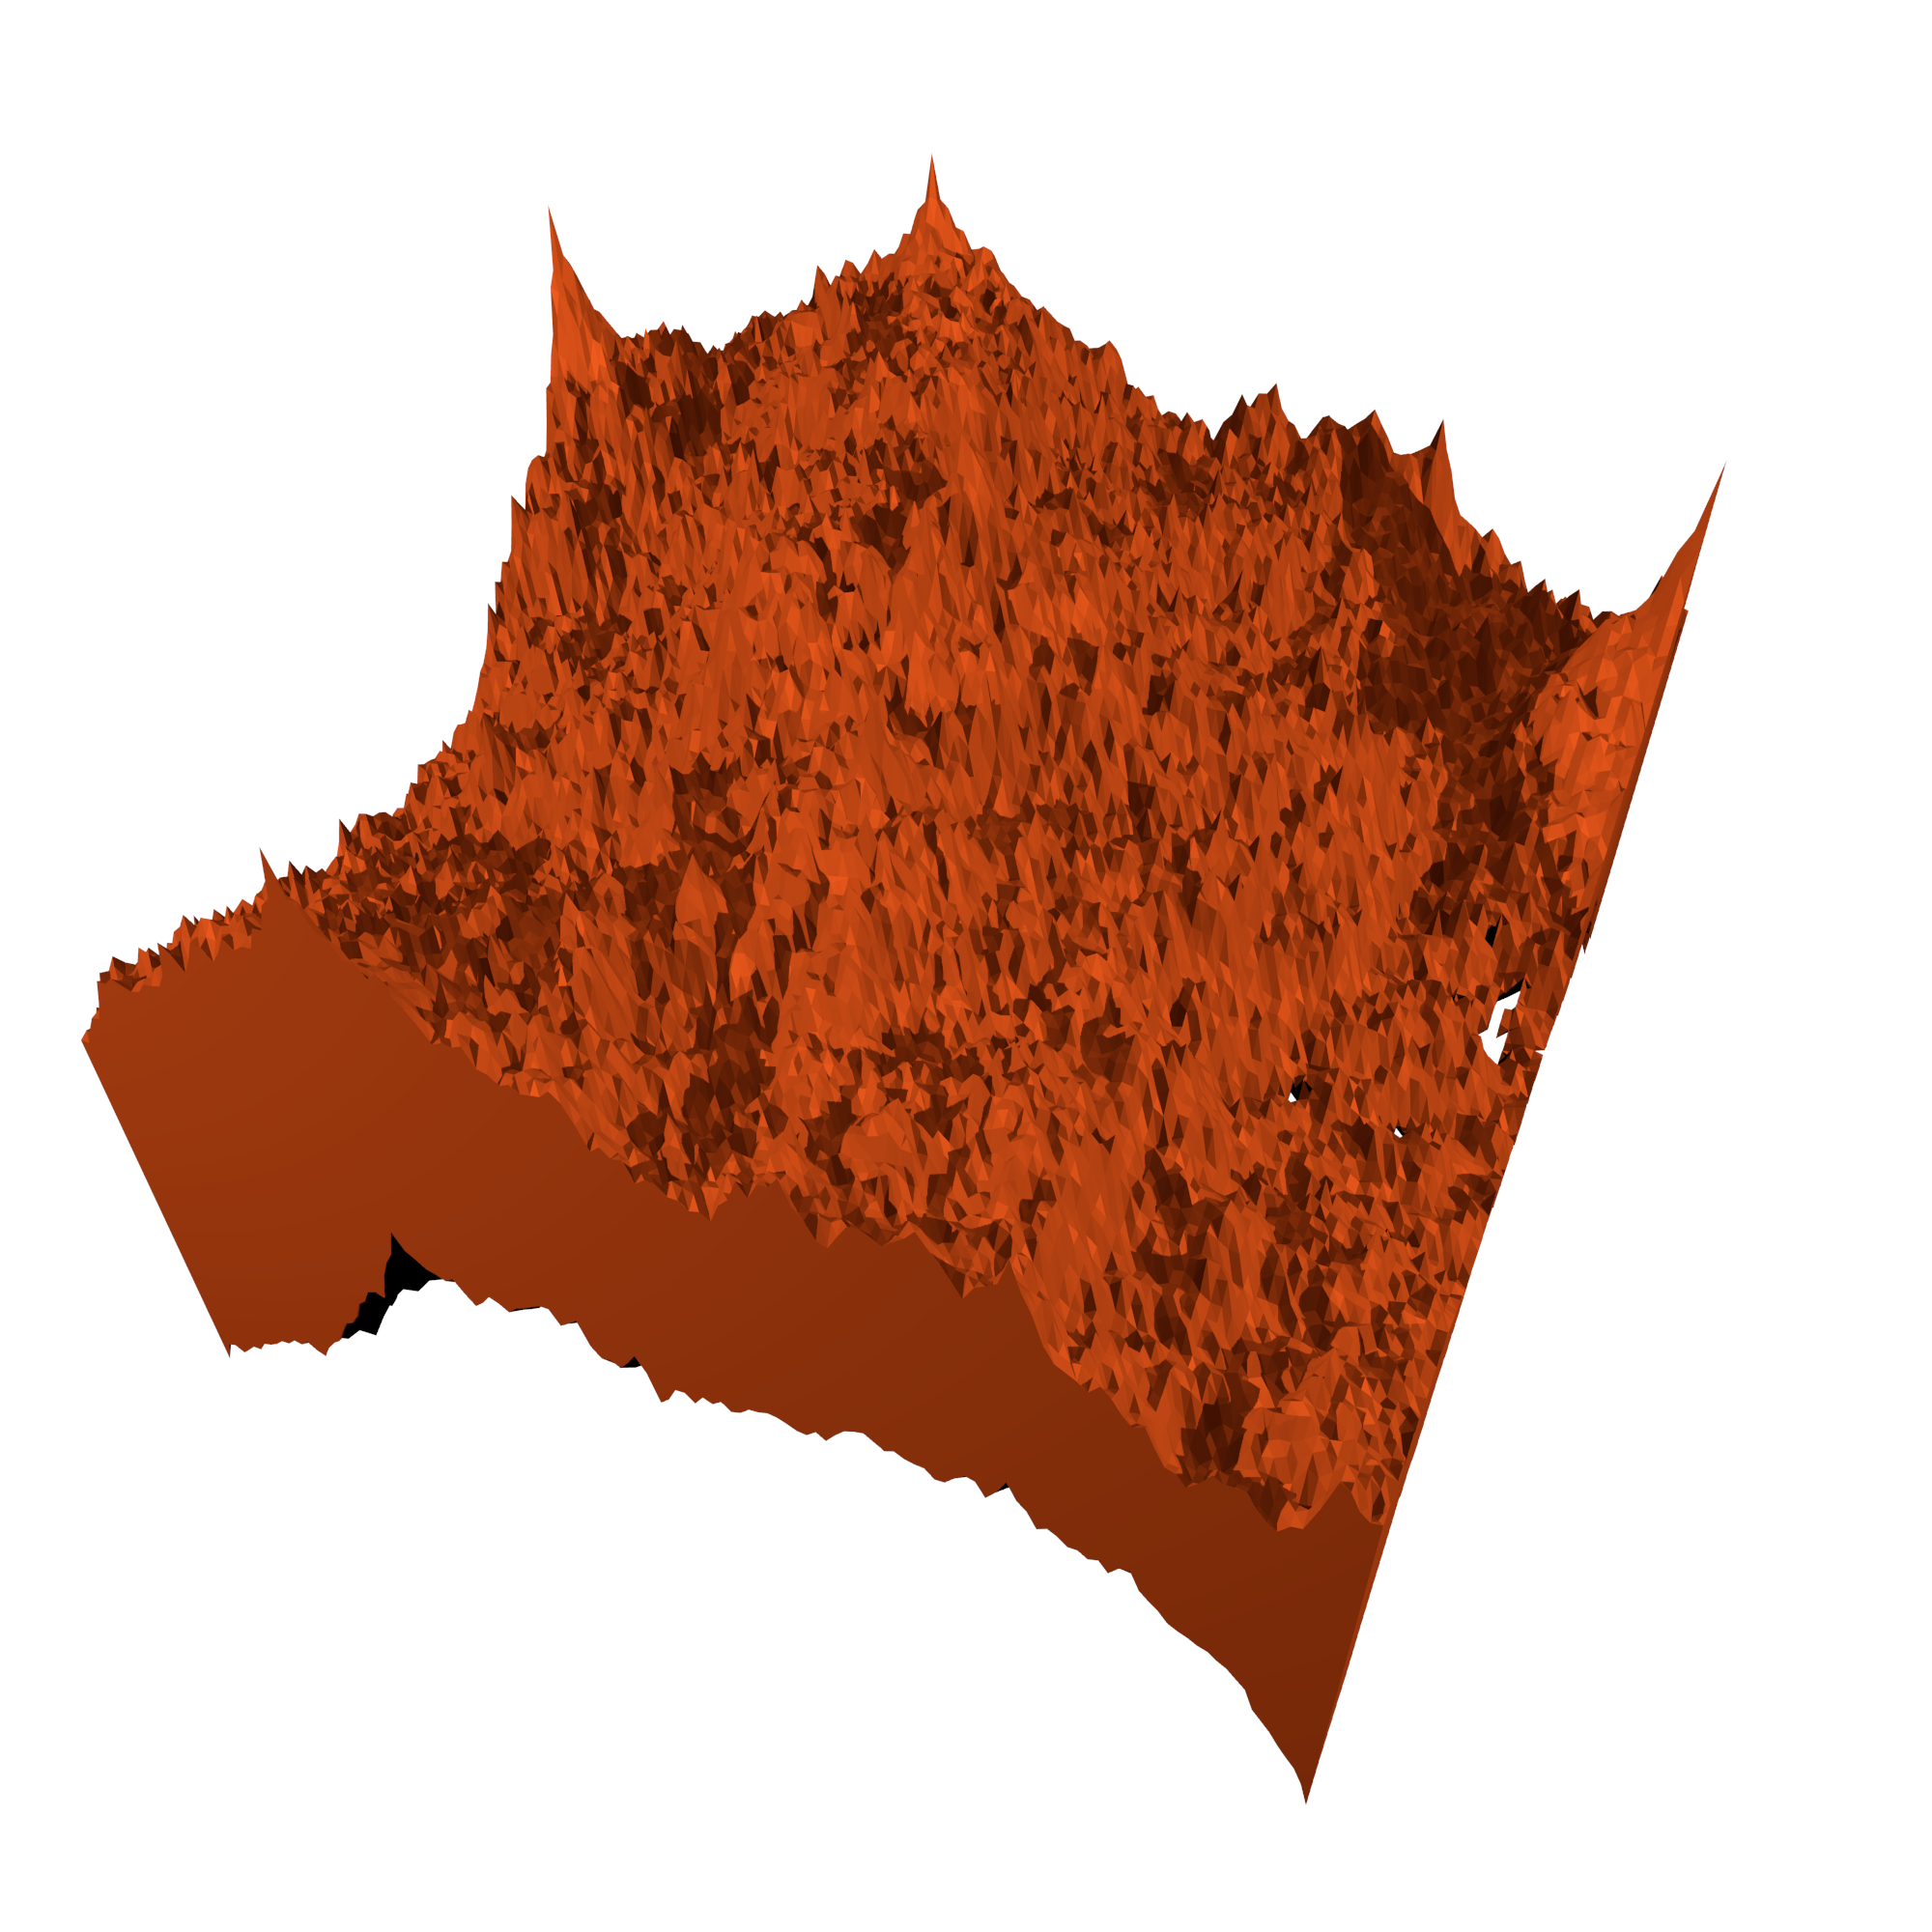
\includegraphics[width=0.6\textwidth]{images/fracture/fracture.png}%
%     \caption{%
%         A model of a fracture.%
%         \label{fig:fracture_model}%
%     }%
% \end{figure}%
%
\begin{figure}[htpb]%
    \centering%
    \setlength{\myfigwidth}{0.4\textwidth}%
%     \setlength{\mycaptionwidth}{0.3\textwidth}%
    \begin{subfigure}[b]{\myfigwidth}%
        \centering% % Need to center to get image centered over caption
        
\includegraphics[width=0.6\textwidth]{images/fracture/hexahedron_to_tetrahedra01_cycles_n200_cropped.png}%
        \caption{Illustration of how to divide a convex hexahedron into five tetraheda.}%
        \label{fig:hex_to_tetra}%
    \end{subfigure}%
    \hspace{0.1\textwidth}%
    \begin{subfigure}[b]{\myfigwidth}%
        \centering%
        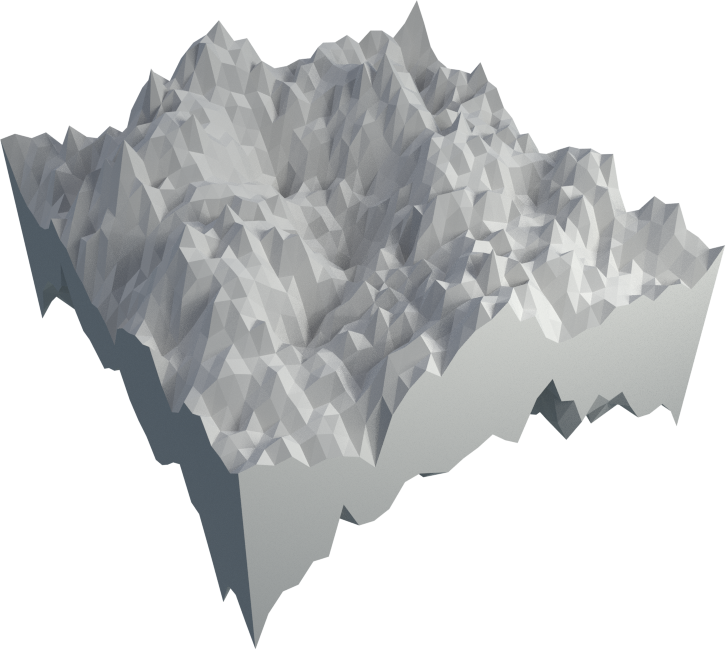
\includegraphics[width=\textwidth]{images/fracture/fracture05_n200_cropped.png}%
%         \includegraphics[width=\textwidth]{images/fracture/large_fracture04_300dpi_w20cm}%
        \caption{A random fracture made from two periodic surfaces.}%
        \label{fig:fracture_model}%
    \end{subfigure}%
\end{figure}%

\part{Experiments}
    \chapter*{Introduction}%
\addcontentsline{toc}{chapter}{Introduction}%
In this chapter we will present the procedure we have used when doing simulations, the systems we have studied, and the the results we have found. 

We start with a description of what steps we have used to generate a realistic nanoporous silica, with water in the pores. We describe how we create a \hl{random} fracture in a slab of silica, and the method we have developed for passivating the dangling ends after we cut out the fracture. We also describe a method for injecting water into the fracture.

After this we present the different measurements we have done during the simulations, how the measurements are done, and why we do them. We then describe the different systems we have generated, the characteristics of these systems, both in form of tables, and using renderings of visualizations of the systems.

Finally the results from all our simulations and measurements are presented and discussed. \todoa{Some more intro to results?}
    \chapter{Doing experiments}
\section{(Initialization) A typical experimental procedure}
When doing \hl{``experiments''} using molecular dynamics we use a procedure \hl{akin to/mimicing} that used by \hl{actual} experiments. Since the duration of the experiments we are realistically able to simulate on are of the order $10^{-9}$ s / nanoseconds or below, we have to be smart when initializing the system, to avoid having to simulate for a long time to get to the state we want to study. This means that we should start out with the system in a configuration/state as close to the one we want to study as possible. The problem with this when simulating \hl{silica/glass} is that the silica structure formed when rapidly cooling molten silica doesn't have any long-range ordering. Silica in the glass form has an amorph structure, which doesn't have any long-range ordering, but has short-range ordering ``well beyond the Si-O bond length''. This structure is hard to set up with an algorithm.
%
% \orangebox{}{
%     \begin{itemize}
%         \item Remove drift!
%         \item Something smart about why the small timescales doesn't matter that much, since the length scales are equally small?
%         \item Short/long-range order
%         \item Glass transition temperature
%     \end{itemize}
%     \begin{quote}
%         ``
%         When molten silicon dioxide SiO2 is rapidly cooled, it does not crystallize but solidifies as a glass. The geometry of the silicon and oxygen centers in glass is similar to that in quartz and most other crystalline forms of the same composition, i.e., silicon is surrounded by a regular tetrahedra of oxygen centers. The difference between the glass and the crystalline forms arise from the connectivity of these tetrahedral units. Although there is no long range periodicity in the glassy network there remains significant ordering at length scales well beyond the SiO bond length. One example of this ordering is found in the preference of the network to form rings of 6-tetrahedra.[18]
%         
%         The glass transition temperature of pure SiO2 is about 1475 K.
%         ''
%         
%         \url{http://en.wikipedia.org/wiki/Silicon_dioxide#Fused_quartz}
%     \end{quote}
% }

To generate silica in the glass form we first create a perfect silica crystal in the crystalline form $\upbeta$-cristobalite, as see in figure \cref{fig:cristobalite} \todo{Why?}, and give the atoms a random uniformly distributed velocities with mean $\mu = 0$ and standard deviation $\sigma = \sqrt{T}$, where $T$ is the wanted temperature \hl{in MD units}. The crystal consists of corner-bonded SiO$_4$ tetrahedra, and in the perfect crystallic form all silicon atoms are bound to four oxygen atoms, and all oxygen atoms to two silicon atoms.
%
\begin{figure}[htpb]%
    \centering%
    \begin{subfigure}[c]{0.25\textwidth}%
%         \begin{minipage}[c]{\textwidth}%
        \includesvg[width=\textwidth, svgpath=./images/beta_cristobalite/]{beta_cristobalite_x01}%
%         \end{minipage}%
%         \caption{\cite{wikiCristobalite01}}%
        \caption{}%
        \label{fig:cristobalite01}%
    \end{subfigure}%
    \hspace{0.07\textwidth}%
    \begin{subfigure}[c]{0.45\textwidth}%
%         \begin{minipage}[c]{\textwidth}%
        \includesvg[width=\textwidth, svgpath=./images/beta_cristobalite/]{beta_cristobalite_xyz01}%
%         \end{minipage}%
%         \caption{\cite{wikiCristobalite02}}%
    \caption{}%
    \label{fig:cristobalite02}%
    \end{subfigure}%
    \caption{%
        Illustrations of the $\upbeta$-cristobalite structure, from two different views. Images from Wikipedia Commons, released to the public domain\cite{wikiCristobalite01,wikiCristobalite02}.%
        \label{fig:cristobalite}%
    }%
\end{figure}%
%
\begin{figure}[htpb]%
    \centering%
    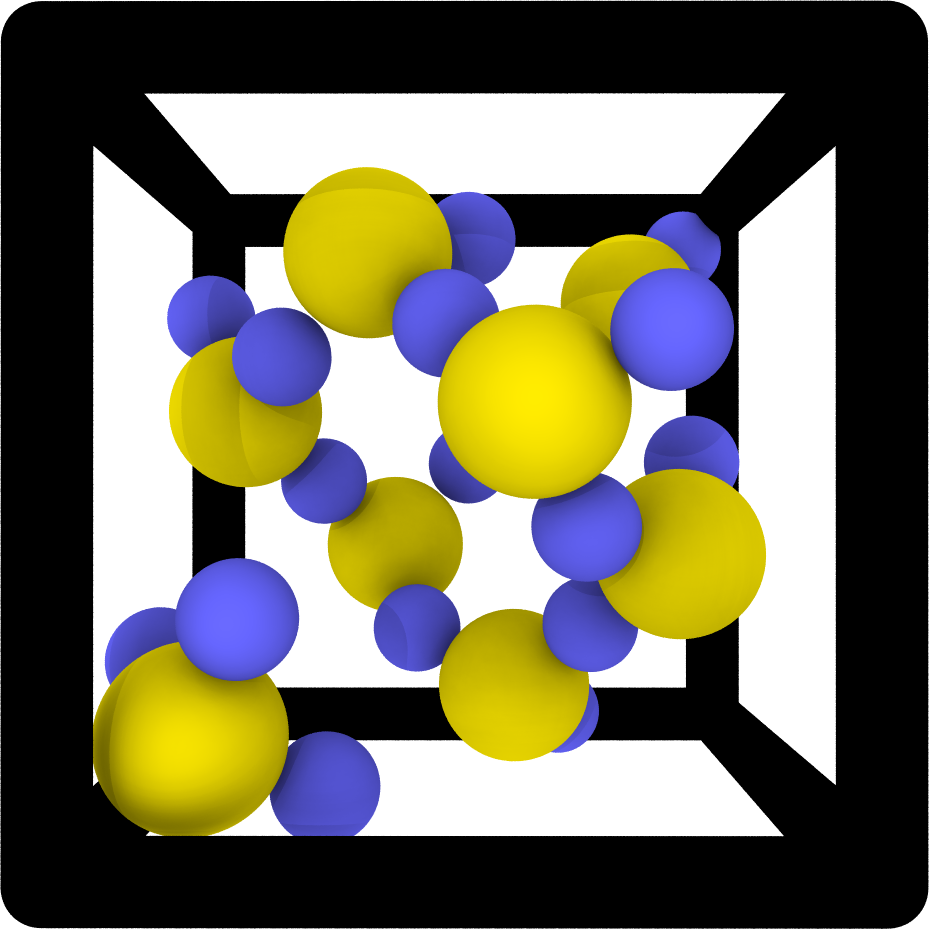
\includegraphics[width=0.6\textwidth]{images/beta_cristobalite/unit_cell03_cropped.png}%
    \caption{
        \hl{FINISH CAPTION}%
    }%
    \label{fig:beta_cristobalite-unit_cell}%
\end{figure}%

We then heat the system to 4500 K in steps of 700 K to melt the silica crystal. We alternate between using a thermostat to adjust the temperature and simulating with the thermostat off to let the system thermalize. The number of timesteps we used for the thermostat period is around 2 500, and for the thermalization period around 10 000. We then cool the system by doing the previous procedure in reverse.

We now have a thermalized and \hl{(hopefully)} realistic silica crystal at near room temperature. From this crystal we cut out the fracture, passivate using one of the passivation methods, and fill the fracture with water molecules, \hl{and use steepest descent}. After filling the fracture with water we need to thermalize the system again, since the energy (and thereby the temperature) changes when we remove and insert atoms.

We are now ready to do measurements.
%
\begin{figure}[htpb]%
    \centering%
    \begin{subfigure}[c]{0.45\textwidth}%
%         \begin{minipage}[c]{\textwidth}%
        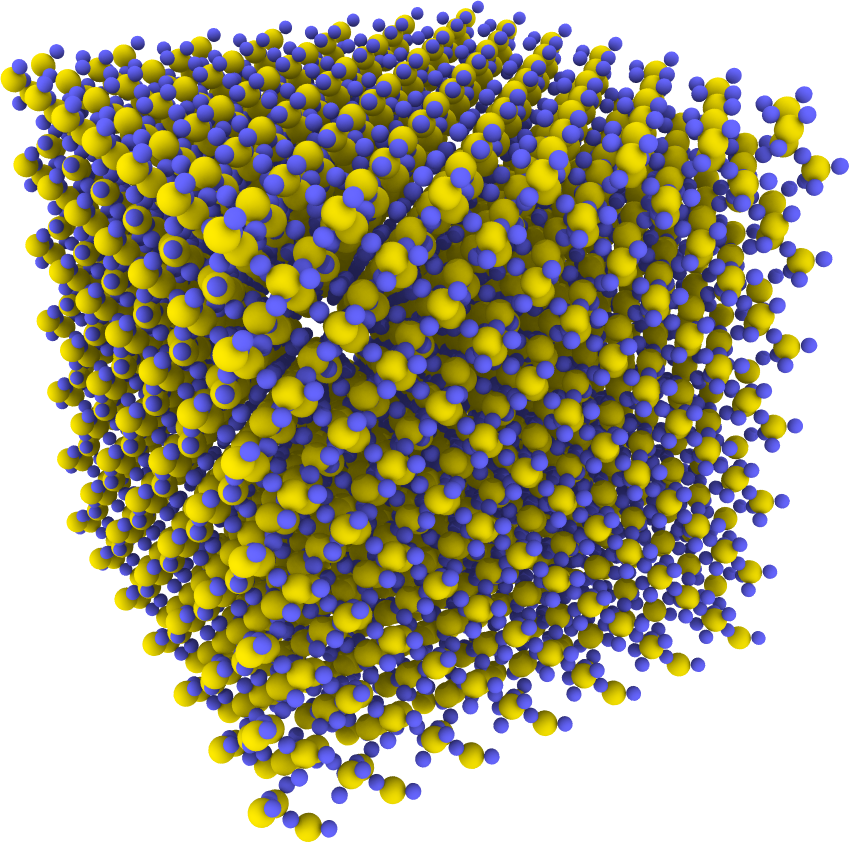
\includegraphics[width=\textwidth]{images/melt_glass/perfect_crystal02_cropped}%
%         \end{minipage}%
%         \caption{\cite{wikiCristobalite01}}%
        \caption{}%
%         \label{fig:cristobalite01}%
    \end{subfigure}%
    \hspace{0.07\textwidth}%
    \begin{subfigure}[c]{0.45\textwidth}%
%         \begin{minipage}[c]{\textwidth}%
        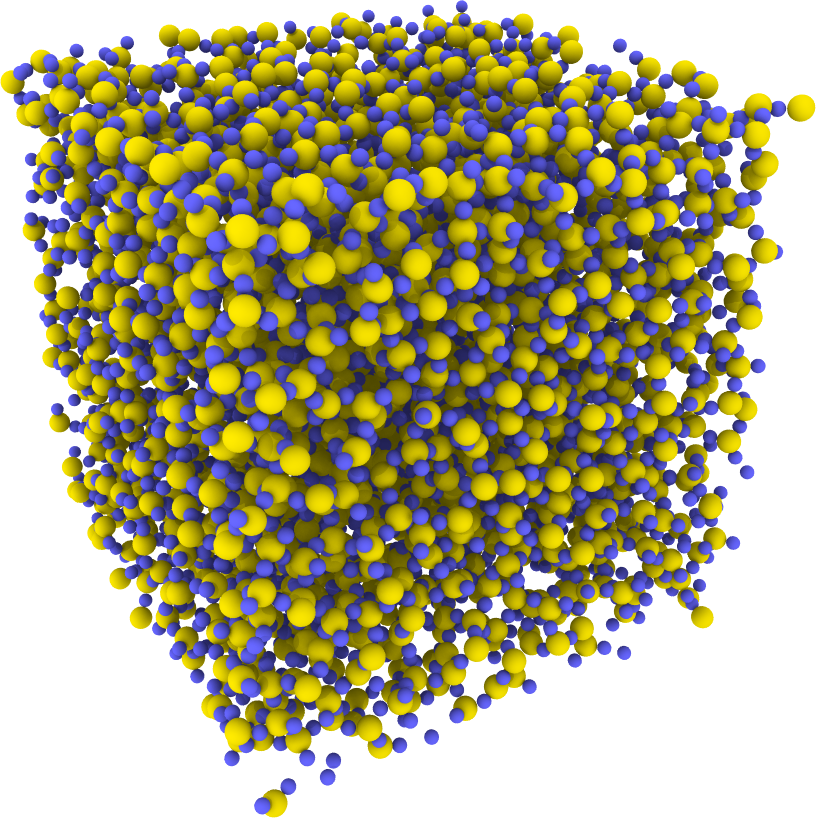
\includegraphics[width=\textwidth]{images/melt_glass/melted02_cropped}%
%         \end{minipage}%
%         \caption{\cite{wikiCristobalite02}}%
        \caption{}%+
%         \label{fig:cristobalite02}%
    \end{subfigure}%
    \caption{%
        Fig%
        \label{fig:melted_glass}%
    }%
\end{figure}%

\section{Passivation}
In most silicates the silicon atoms have tetrahedral coordination, with four oxygen atoms surronding each silicon atom. When we remove silica- and oxygen-atoms to create a fracture, we don't take this into consideration. This means that we get dangling unsaturated bonds in the system, located near the surface of the pore. To rectify this we use a method called passivation, where we saturate \hl{and passivate} the dangling bonds by inserting new atoms. 

\subsection{Water chemistry}
Since we are going to inject water into the pore later on, we want to use the constituents of water to passivate the system. We know that water autodissociates into H$^{+}$ and OH$^{-}$ via the following reaction
\begin{align*}
    \text{H}_2\text{O} \rightleftharpoons \text{H}^{+} + \text{OH}^{-},
\end{align*}
meaning that hydrogen (H) and hydroxide (OH) will be freely available in the system after filling the pore with water. On this background we choose to passivate the system using hydrogen and hydroxide. To avoid getting an \hl{acidic or alkaline / charged?} system after the passivation procedure we should make sure to use equal parts hydrogen and hydroxide when passivating.\todo{we don't whink of this when cutting though...}

\subsection{Passivating using hydrogen and hydroxide}
After thermalizing our silica system we end up with a system consisting almost exclusively of SiO$_2$ tetrahedra\todo{source? what is the rest?}. These tetrahedra are each formed by four oxygen atoms, one in each corner, and a silicon atom in the center. Each of these tetrahedra are then bonded to four other tetrahedra, by sharing the oxygen atoms in the corners. This way each oxygen atom is bonded to two silicon atoms, and each silicon atom to four oxygen atoms, giving an average chemical \hl{formula} of SiO$_2$. 

Since we don't take \hl{chemical bonds (we have no bonds...)} into consideration when removing atoms to create a fracture, we end up with some incomplete tetrahedra, with some silicon atoms bonded to less than four oxygen atoms, and some oxygen atoms bonded to less than two silicon atoms. See \cref{fig:passivation} for an illustration of three different incomplete tetrahedra. This creates what we call dangling ends/unsaturated bonds, which we want to \hl{remove/passivate}.

% When inserting hydrogen and hydroxide we want to insert them in positions that are close to their equilibrium positions, so we don't have to do a lot of simulating to get a stabilized system after passivating. It's possible to calculate the optimal positions based on the potential and the positions of the existing atoms, but this is a complicated computation, that we can avoid, by instead realizing that the optimal positions for the oxygen atoms we insert will most likely \hl{(source?)} be close to the positions that complete the SiO$_2$ tetrahedra. These positions can be calculated, using simple geometry, from the positions of the oxygen atoms each silicon atom is bonded to.

To passivate the silicon atoms that are \hl{bonded} to less than four oxygen atoms, we see that we need to complete the incomplete SiO$_4$ tetrahedra that have been created in the system. But if we only insert oxygen atoms in the positions of the missing oxygen atoms, we end up with new dangling \hl{ends/bonds}, since the inserted oxygen atoms will only be bonded to one silicon atom. But, as we just saw, we will have hydroxide (OH) groups available in the system after filling the fracture with water. So instead of inserting oxygen atoms and creating new unsaturated bonds, we insert hydroxide groups and create saturated Si-O-H \hl{bonds}. \hl{ SiO$_n$(OH)$_{4-n}$ tetrahedra.} We put the hydrogen atom so that the Si-O-H angle is close to the angle in water molecules, 107.5 degrees. \hl{The hydrogen atoms moves very rapidly compared to the rest of the species in the system, so they will quicly find the equilibrium position.}

To passivate the oxygen atoms that are bonded to only one silicon atom, we can use the hydrogen atoms that are avilable after filling the fracture with water, turning unsaturated SiO-groups into the same saturated Si-O-H-groups as before. We here too insert the hydrogen atoms with the Si-O-H angle close to 107.5 degrees.

In total we use the following procedure to passivate a system after creating a fracture:
\begin{itemize}
    \item Remove all silicon and oxygen atoms that aren't bonded to any atoms, since they are \hl{essentially} not part of the silica \hl{crystal/matrix}.
    \item Add one hydrogen atom to all oxygen atoms bonded to only one silicon atom. The hydrogen atoms are inserted approximately $0.95\text{ \AA}$ from the oxygen atoms, with the hydrogen atom pointing away from the silicon atom, and with the Si-O-H angle close to 107.5 degrees.
    \item Add ($4-n$) hydroxide \hl{molecules/groups} to silicon atoms bonded to $(1\leq n<4)$ oxygen atoms. We assume that the most stable position for the oxygen in the hydroxide groups are close to the tetrahedral positions of the missing oxygen atoms, and insert the hydroxide groups in these positions. %
    %See \cref{fig:pass_tet01,fig:pass_tet02,fig:pass_tet03} for the three different cases. 
    The hydroxide groups are inserted approximately $1.65\text{ \AA}$ from the silicon atoms, measured from the position of the silicon atom to the oxygen atom in the hydroxide groups, with the hydrogen atom pointing away from the silicon atom, and with the Si-O-H angle close to 107.5 degrees.
\end{itemize}
The lengths used are approximate experimental lengths found in naturally occuring silanols and water (see \cite{lickiss1995synthesis} for the Si-O length in silanol, and \cite{csaszar2005equilibrium} for the O-H length in water). This procedure turns all dangling ends into \hl{stable, passive} silanol groups.
%
\begin{figure}[htpb]%
    \centering%
    \begin{subfigure}[b]{0.24\textwidth}%
        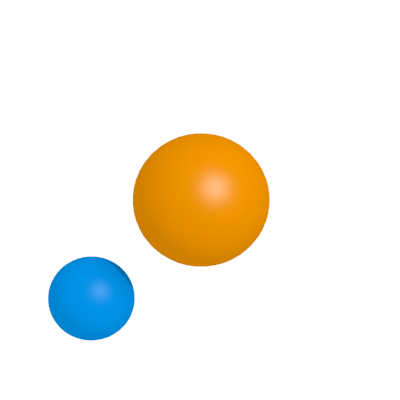
\includegraphics[width=\textwidth]{images/passivation/tetrahedra01.png}%
        \caption{}%
%         \caption{Illustration of how to divide a convex hexahedron into five tetraheda.}%
        \label{fig:pass_tet01}%
    \end{subfigure}%
%     \hspace{5mm}%
    \begin{subfigure}[b]{0.24\textwidth}%
        
\includegraphics[width=\textwidth]{images/passivation/tetrahedra02.png}%
        \caption{}%
%         \caption{A random fracture made from two periodic heightmaps.}%
        \label{fig:pass_tet02}%
    \end{subfigure}%
%     \hspace{5mm}%
    \begin{subfigure}[b]{0.24\textwidth}%
        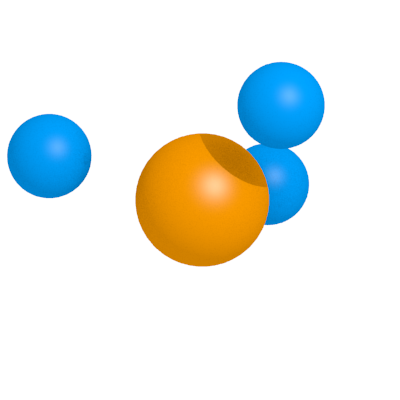
\includegraphics[width=\textwidth]{images/passivation/tetrahedra03.png}%
        \caption{}%
%         \caption{A random fracture made from two periodic heightmaps.}%
        \label{fig:pass_tet03}%
    \end{subfigure}%
%     \hspace{5mm}%
    \begin{subfigure}[b]{0.24\textwidth}%
        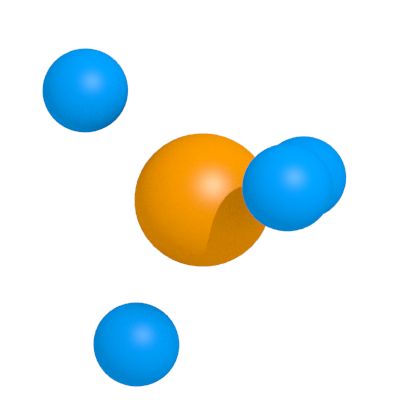
\includegraphics[width=\textwidth]{images/passivation/tetrahedra04.png}%
        \caption{}%
%         \caption{A random fracture made from two periodic heightmaps.}%
%         \label{fig:fracture_model}\caption{}%
    \end{subfigure}%
    \caption{%
        Illustration of four different incomplete silica tetrahedra, with respectively one, two, and three missing oxygen atoms. \hl{UNNECESSARY FIGURE?}
    }%
    \label{fig:passivation}%
\end{figure}%

% \begin{itemize}
%     \item Oxygen atoms with less than two silicon neighbor
%     \item Silicon atoms with less than four oxygen neighbors.
%     \item Oxygen atoms with one missing silicon neighbor.
%     \item Silicon and oxygen atoms with no neighbors.
%     \item \hl{Silicon and oxygen atoms with too many neighbors?}
% \end{itemize}

% In the passivation procedure we do some basic assumptions, based on the chemical nature of silica and water. In the thermodynamically stable form, silica should have the following properties\todo{source?}:
% \begin{itemize}
%     \item Silicon atoms should have tetrahedral coordination, with four oxygen atoms surrounding each silicon atom in a tetrahedral \hl{shape}. \todo{On average, not all silica will have this. Something about bonds? bonded to four oxygen atoms?}
%     \item Oxygen atoms should have two silicon \hl{neighbors}\todo{not all, on average}.
%     \item The Si-O distance should be in the range 1.5-1.9 pm\todo{source?} (depending on the crystalline form).
% \end{itemize}

% \hl{When removing atoms to create pores we don't care about these properties, which leads us to the following cases}


% \hl{When inserting oxygen and hydrogen we must make sure to inject neutrally, meaning twice as much hydrogen as oxygen (H$_2$O)}

% Silicon atoms with less than four oxygen atoms bound to them get ($4-n_\text{O}$) hydroxide (OH$^-$) groups attached to them, where $n_\text{O}$ is the numer of oxygen atoms bound to the silicon. Oxygen atoms with a missing silicon neighbor get a hydrogen attached. 
% % \hl{(oxygen atoms with two missing neighbors are removed)}.
% % Oxygen atoms with less than two silicon atoms get ($2-n_\text{Si}$) hydrogen atom attached, where $n_\text{Si}$ is the number of silicon atoms bound to the oxygen. 
% 
% When passivating a silicon atom with missing oxygen neighbors by \hl{simply} filling in the missing atoms to complete the SiO$_4$-tetrahedra. We then put one hydrogen atom on each new oxygen atom, to avoid dangling bonds on the inserted oxygen atoms.
% 
% When passivating a oxygen atom with a missing silicon neighbor, we put one hydrogen atom on the opposite side of the oxygen atom compared to the silicon atom.
% 
% All silicon and oxygen atoms with no neighbors we remove, since they aren't really part of the silica.

\subsection{Counting number of bonds}
Since we don't have actual bonds in molecular dynamics simulations, we don't know what the actual bonds look like. So to find the number of \hl{neighbors/bonds/bonded atoms} for each silicon and oxygen atom, we create what we call \emph{neigbor lists}, which is a list of atoms within a chosen radius, for each atom. To create these lists we use the procedure detailed in \cref{sec:neighbor_lists}. Since we only have silicon and oxygen atoms in our system, we only need to specify a maximum the Si-O-distance to find which atoms are bonded. If we choose this distance properly, we should be able find a good approximation to how many atoms each atom is bonded to.

\orangebox{
\begin{itemize}
    \item What Si-O distance did we use to find bonds? Why? 
    \item g(r) for Si-O?
    \item Implementation?
    \item Visualization of results?
    \item What to do about atoms that can't be passivated (because we have to insert passively)?
\end{itemize}
}

% \subsection{Implementation}
% To implement the passivation procedure detailed above we see that we can make an  

% \begin{itemize}
%     \item Tetrahedra
%     \item Neighbor lists -- see base\_code/passivate\_using\_tetrahedra/passivator.cpp near line 700
%     \begin{itemize}
%         \item Create list of atoms in each voxel
%         \item Create neighbor lists for each atom by looping through neighbor voxels for each atoms
%     \end{itemize}
%     \item Count number of neighbors of different types -- find number of missing neighbors, Si - 4 Oxygen, Oxygen 2 Si
%     \item Insert OH on Si with missing O neighbors, insert H on Oxygen with missing Si neighbors
%     \begin{itemize}
%         \item Insert O/H at good angles
%     \end{itemize}
%     \item Improvement: find the atoms near surface using voxels, only passivate those atoms
% \end{itemize}

\subsection{Only passivating surface atoms}
When implementing the passivation method detailed above, we soon ran into problems with silica and oxygen atoms that were bonded to too few atoms according to our rules above, while counting the number of bonds using a fixed radius. Some improvements were made by fine-tuning the radius used for each atom type, but we still often ended up passivating atoms that were inside the silica matrix, where we shouldn't have any dangling \hl{bonds/ends}. To avoid this we came up with a method to only passivate the atoms \hl{at or near} the surface of the fracture.

To do this we \hl{yet again} use the voxelation method from \ref{sec:voxelation}, but this time we use a voxel size of around $6\text{ \AA}$. We then mark all voxels with atoms in them as occupied. We now see that if we find all \emph{occupied} voxels with at least one \emph{unoccupied} neighbor voxel \hl{(using 26-neighbor connectivity)}, we should have a list of the voxels that make up the surface of the fracture, and these voxels then contain all atoms at or near the surface of the fracture. We then use this list of atoms as input to the passivation program, and only passivate atoms in that list. See \cref{fig:find_surface_atoms} for an illustration of the method that finds the voxels and atoms at the surface of the fracture.
%
\begin{figure}[htpb]%
    \centering%
    \includesvg[width=0.5\textwidth, svgpath = ./images/passivation/]{select_surface_voxels05}%
    \caption{
        Illustration of a method for finding atoms and voxels at the surface of a fracture. All gray voxels are occupied voxels (with at least one atom in them), and the dark gray voxels are the voxels with at least one unoccupied neighbor voxel. \hl{FINISH} \hl{change to v1 of illustration?} \hl{what size shoud fig be? 0.4 maybe a bit small?}
    }%
    \label{fig:find_surface_atoms}%
\end{figure}%

\subsection{Results/examples}
An example of a system after passivation can be seen in \cref{fig:passivation_example}. Here we see hydrogen and ???
%
\begin{figure}[htpb]%
    \centering%
    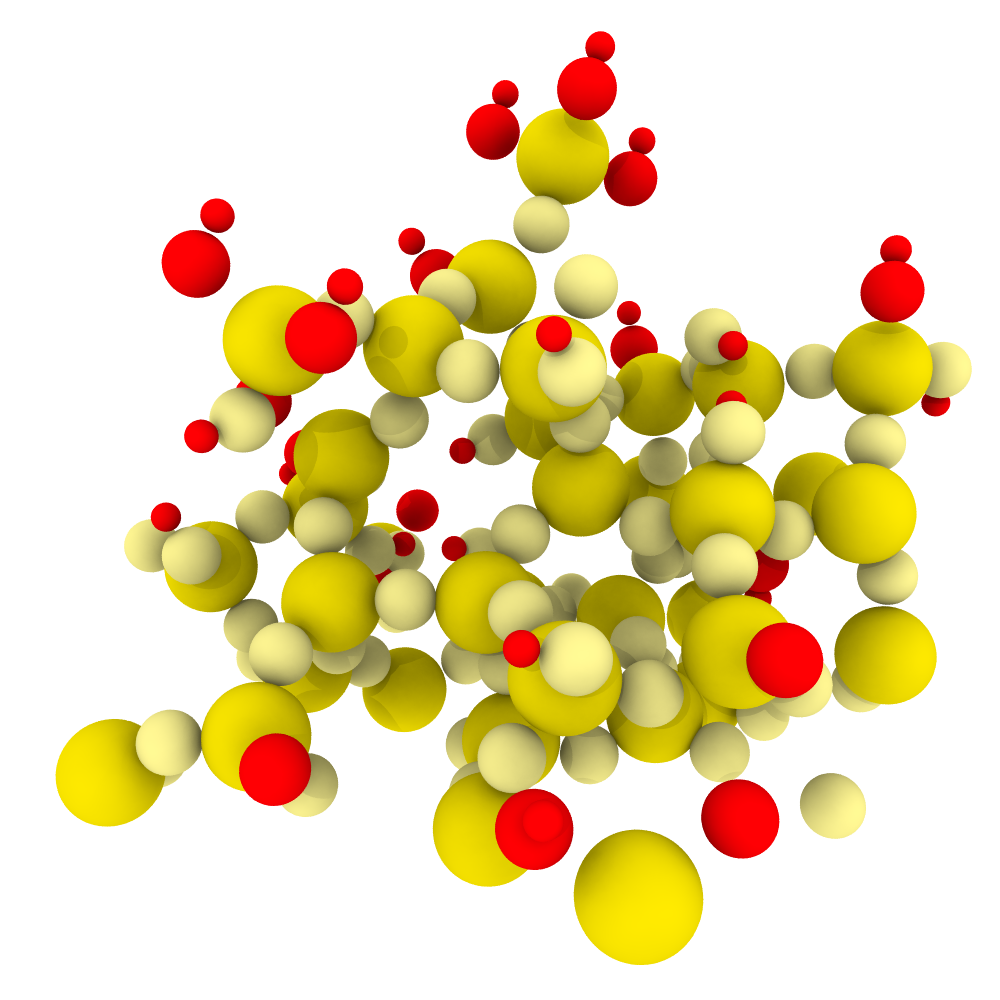
\includegraphics[width=0.7\textwidth]{images/passivation/passivation_example04.png}%
    \caption{
        Passivation example.png.\hl{FINISH CAPTION}%
    }%
    \label{fig:passivation_example}%
\end{figure}%

\FloatBarrier
\section{Injecting water}
After removing atoms to create a fracture, and passivating the system, we are now ready to inject water into the fracture. To do this we use the technique of \emph{voxelation} (see \cref{sec:voxelation}). We first divide the system into voxels, find the empty voxels, and then put one water molecule in each unoccupied voxel. The water density can then be controlled by the size of the voxels we use.\todo{Not filling all voxels}

\subsection[Finding correct voxel size/water density?]{Finding correct voxel size/\hl{water density?}}
If we want to inject water with density $\rho$% [kg/m$^3$]
, we can find the voxel size we need from the molar mass of water, $M_\text{H$_2$O} = M = 0.0180158 \text{ kg/mol}$\hl{SOURCE}. We use the molar mass and wanted density to find the ``volume'' each water atom should occupy% , the unit used in the \hl{MD integrator/program and output files}
, as follows
% \begin{align*}
%     V 
%     &= \frac{ M\text{ [kg/mol]} }{ \rho\text{ [kg/m$^3$]} } \\
%     &= \frac{
%             M\text{ [kg/mol]} \times \dfrac{1}{N_A \text{ [mol$^{-1}$]}}
%         }{
%             \rho\text{ [kg/m$^3$]} \times \left(10^{-10} \text{ [\AA/m]}\right)^3
%         } \\
%     &= \frac{M}{\rho} \times \frac{10^{-30}}{N_A} \text{ [\AA$^3$]},
% %     \times \frac{N_A \text{ [mol$^{-1}$]}}{10^{-10} \text{ [\AA/m]}} 10 \text{ [m$^3$]} \\
% \end{align*}
\begin{align*}
    V 
    = \frac{ M\text{ [kg/mol]} \times \dfrac{1}{N_A \text{ [mol$^{-1}$]}}}{ \rho\text{ [kg/m$^3$]} } 
    = \frac{M}{\rho N_A}\text{[m$^3$]}
\end{align*}
where $N_A$ is the Avogadro constant. From here we find the size we need our voxels by taking the cube root
% \begin{align*}
%     l = \left(\frac{M}{\rho} \times \frac{10^{30}}{N_A}\right)^{1/3}\text{ [\AA]}.
% \end{align*}
\begin{align*}
    l = \left(\frac{M}{\rho N_A} \right)^{1/3}\text{ m}.
\end{align*}
We then divide the system into voxels of length $l$, and put one water molecule with random orientation in the center of each empty voxel. If we for example want to insert water with $\rho = 1000\text{ kg/m}^3$, approximately the density of water in room temperature\hl{SOURCE}, we get a voxel size of
\begin{align*}
    l = \left(\frac{0.0180158 \text{ kg/mol}}{1000\text{ kg/m$^3$} \times 6.0221 \times 10^{23}\text{ mol$^{-1}$}} \right)^{1/3} = 3.1 \text{ \AA}.
\end{align*}

\subsection{Finding empty voxels}
The naive way of finding the empty voxels is to just find which voxel each silicon and oxygen atom is in, and mark those as occupied. Using this method we found that we often got some empty voxels inside the silica matrix, which meant we got single water atoms trapped inside what was supposed to be the silica matrix. 

This can be explained if we compare the voxel size of $3.1 \text{ \AA}$ in water with a density of $\rho = 1000\text{ kg/m$^3$}$, as we found above, to the typical Si-O bond length in silica. \todo{better explanation}When we take into account the amorphous structure of silica we see that it's likely that we get some small pores with room for a water atom in between some of the silica tetrahedra.

To solve this we assign a radius to each atom type\todo{which is hard, Si-O, ???}, and mark all voxels with the center of the voxel within this radius from an atom as occupied. See \cref{fig:inject_empty_voxel} for an illustration of this procedure. 
%
\begin{figure}[htpb]%
    \centering%
    \begin{subfigure}[b]{0.45\textwidth}%
        \includesvg[width=\textwidth, svgpath=./images/inject_water/]{drawing02}%
%         \caption{}%
        \caption{Marking only one voxel per atom as occupied.}%
%         \label{fig:pass_tet01}%
    \end{subfigure}%
    \hspace{0.05\textwidth}%
    \begin{subfigure}[b]{0.45\textwidth}%
        \includesvg[width=\textwidth, svgpath=./images/inject_water/]{drawing_radius02}%
%         \caption{}%
        \caption{Marking all voxels within radius from atom as occupied.}%
%         \label{fig:pass_tet02}%
    \end{subfigure}%
    \caption[
        To find voxels we can put water molecules in we can either \textbf{a)} mark the voxel each atom belongs in as occupied, or \textbf{b)} mark all voxels within a radius from each atom as occupied. We can assign a different radius to each atom. We have illustrated using part of a silica tetrahedra, with one silicon atom (the large blue dot) and two oxygen atoms (the smaller red dot). The center of each voxel is marked by a dot 
    ]{%
        To find voxels we can put water molecules in we can either \textbf{a)} mark the voxel each atom belongs in as occupied, or \textbf{b)} mark all voxels within a radius from each atom as occupied. We can assign a different radius to each atom. We have illustrated using part of a silica tetrahedra, with one silicon atom (
\includegraphics[scale=0.8]{./images/inject_water/silicon.pdf}) and two oxygen atoms (\raisebox{0.3ex}{
\includegraphics[scale=0.8]{./images/inject_water/oxygen.pdf}}). The center of each voxel is marked by a dot. \hl{Maybe change to v01 of images?} \hl{This voxel size is pretty tiny...}
    }%
    \label{fig:inject_empty_voxel}%
\end{figure}%

A different solution to the problem of tiny pores inside the silica matrix is to \hl{just} remove all small clusters of voxels (where a ``small cluster of voxels'' would need to be defined)\hl{, which sometimes can be a better solution, since we introduce new lone voxels when making radius? Maybe implement both methods, a small radius and remove small clusters?}.

\orangebox{
\begin{itemize}
    \item Remove tiny pores?
    \item Mark all voxels within distance from other atoms as occupied
    \item Fill other voxels with H2O with random O-H orientation, but correct angle
    \item Improvement: Use one voxel size in the beginning (to avoid one-voxel pores), and then use a smaller voxel size when injecting water
\end{itemize}
}


    \chapter{Other measurements???}
% \section{Voxelation, calculating distances, finding neighbors, neighbor lists, periodicity tricks\label{sec:voxelation}}

\section{Measuring as function of distance from matrix}
\todoa{Finish measuring as function of distance from matrix}
% Mean distance from matrix in range --> if we limit the standard deviation as well, we're effectively limiting temperature, or diffusion??
% When measuring things like density, diffusion, and the tetrahedral order parameter in a nanoporous system, we often want to study the behaviour of 

When doing experiments with nanoporous and nanoscale systems we often want to do measures as function of the distance to the surface of the pore, in our case meaning the distance to the interface between water and silica. The first problem with this is to find out how to measure the distance from a point, for example a water molecule, to the surface. Most of our measures are done on water molecules in fractures and pores, so we first define the position of the water molecule as equal to the position of the oxygen atom in the water molecule\footnote{\hl{Something about using positions of hydrogen atoms as well as oxygen position to define water position?}}. We then use the distance from these water-oxygen atoms to the nearest silica atom to define a distance from the water molecule to the surface of the \hl{pore/fracture}. Finding the nearest silica atom isn't trivial, so a procedure for doing this is shown in \cref{sec:find_distance_to_surface}.

When measuring \hl{things} that only depend on data from one timestep we don't have to worry about that the atoms move, so we just sort the atoms by distance to the surface using the procedure in \cref{sec:find_distance_to_surface} and do our measurements, individually on each timestep. But if we want to study for example diffusion, or the tetrahedral order parameter, which depend on data from several timesteps, we have to find a good way to define which atoms are in a certain range of the surface. We tried different methods, but decided to use the average distance to the surface for this\todobo{why, examples of tested methods}.

\section{Voxelation\label{sec:voxelation}}
The method of voxelation is a method where we divide our simulation system into adjacent boxes or \emph{voxels} (3-dimensional pixels). The system is divided into $n_x\times n_y\times n_z$ voxels of size $l_x\times l_y\times l_z$. Depending the what we want to calculate we can calculate the voxel size from the number of voxels, or vice versa, using the following relation
\begin{align*}
    n_i = \frac{L_i}{l_i},
\end{align*}
where $L_i$ is the system size, assuming that the voxel size $l_i$ is set so that $L_i$ is evenly divisible by $l_i$, that the remainder of $L_i/l_i$ is zero. If we have a maximum or minimum voxel size $l_i^\text{max}$ or $l_i^\text{min}$ we can use the following relations to calculate the number of voxels
\begin{align*}
    &n_i=\left\lfloor\frac{L_i}{l_i^\text{max}}\right\rfloor &\text{or}& &n_i=\left\lceil\frac{L_i}{l_i^\text{min}}\right\rceil,
\end{align*}
where $\lfloor x \rfloor$ is the \Verb!floor!-function and $\lceil x \rceil$ is the \Verb!ceil!-function.

The voxels are indexed $(i,j,k)$ where $i,j,k \in [0,n_i-1]$, and a voxel is defined as the points $(x,y,z)$ where
\begin{align}
    \left\lfloor\frac{x}{l_x}\right\rfloor = i,\label{eq:find_voxel_index}
\end{align}
and similarly for the other dimensions.

\subsection{Neighbor lists\label{sec:neighbor_lists}}
When doing calculations and measurements on a molecular system, we often need information about the neighboring atoms of each atom, and we want to make a so-called \emph{neighbor list}, which are lists of which atoms are within a distance $dr$ of each atom. Finding out which atoms are within a certain distance of each atom can take a long time; the trivial way of checking each atom against all other atoms scales as $\mathcal{O}(N^2)$, $N$ being the number of atoms. 
%
%There are many clever algorithms for finding nearest neighbors, often called a ``nearest neighbor search'' (see \url{http://www.slac.stanford.edu/cgi-wrap/getdoc/slac-r-186.pdf} and references in that paper, especially ``11. Levinthal 1966''). 

Since we want to find all neighbors within a distance $dr$ of a point, for all or most of the atoms, we can use the voxelation method to do it efficiently. To do this we first voxelate the system using a minimum voxel size equal to $r$. We then find which voxel each atom belongs to, and store this. We can then find the atoms within a distance $dr$ from a point $(x,y,z)$ by first finding the voxel this point lies in using (from \cref{eq:find_voxel_index})
\begin{align*}
    &i = \Bigg\lfloor \frac{x}{l_x} \Bigg\rfloor,& &j = \Bigg\lfloor \frac{y}{l_y} \Bigg\rfloor,& &j = \Bigg\lfloor \frac{z}{l_z} \Bigg\rfloor,&
\end{align*}
where $l_x\times l_y \times l_z$ is the actual voxel size (we need an even number of voxels, so the actual voxel size is governed by the system size). We then check the distance between the point and the atoms in the voxel the point belongs in, and the atoms in the 26 neighboring voxels of this voxel. 
\todoc{make voxel size vs. $dr$ illustration}%

Checking the 26 neighboring voxels ensure that we included all atoms within the distance $dr$. We can see this by looking at the worst case example, where we have a point right at the edge of the voxel it belongs to, at $(i+(1-\epsilon_0))$, and an atom in voxel $(i+2)$ being as close to the point as possible, at $(i+2 + \epsilon)$. The distance between those two points would then be
\begin{align*}
    ((i+2)l + \epsilon_1) - (il + (l-\epsilon_0)) 
    &= ((i + 2) - (i + 1) - \epsilon_0)l + \epsilon_1 + \epsilon_0 \\
    &= l + \epsilon + \epsilon_0,
\end{align*}
which is larger than $l$, since $\epsilon_0, \epsilon_1$ have to be larger than 0.

When voxelating the system using the distance $r$ we should take care not to use a too small distance, i.e. make the voxels too small and create a lot of voxels. Since the total number of voxels goes as $n^3$ the memory needed to store the matrix increases rapidly with decreasing voxel size. To avoid this we usually implement a hard limit to the number of voxels, and found that a limit of $n < 256$ or even $n < 128$ seemed to work good in most cases. On the other hand, if we make the voxels too large we soon find that the program isn't especially efficient. This is because most voxels will have a lot of atoms in then, and we have to look through a lot of atoms when checking the 26+1 voxels for each atom.

An implementation of the voxelation method for creating neighbor lists can be seen in \cref{list:create_neighbor_lists}. Note that when calculating distances between points we usually calculate and compare squared distances like $r^2 = (x_1-x_2)(x_1-x_2) + \dots$, since calculating roots are a time-consuming operation on a computer (at least compared to multiplication and addition).
%
% We didn't find any algorithms for solving this specific problem, and the usual algorithms can't benefit from the fact that we need to find the nearest neighbors of \emph{all} points.
%
\begin{listing}[!htb]%
\begin{cppcode*}{gobble=4}
    int nVoxels = floor(systemSize/radius);
    double voxelSize = systemSize*nVoxels;
    
    sortAtomsIntoVoxels(atoms, voxelSize, voxels);
    
    vector<vector<Atom*> > neighborAtoms(atoms.size());
    
    // Loop over all atoms
    for (Atom *atom : atoms)
    {
        // Index of the voxel this atom belongs to
        ivec3 index = floor(atom.position() / voxelSize)
        
        // Loop over all 27 neighbor voxels (including self)
        for (int di = -1; di <= 1; di++)
        for (int dj = -1; dj <= 1; dj++)
        for (int dk = -1; dk <= 1; dk++)
        {{{
            // Index of neighbor voxel using periodic boundary conditions
            // nx, ny, nz is the number of voxels in each direction
            int i = (index[0] + di + nx) % nx;
            int j = (index[1] + dj + ny) % ny;
            int k = (index[2] + dk + nz) % nz;
            
            neighborAtoms[atom.index()].push_back(
                findAtomsWithinRadius(atom, voxels[i][j][k], radiusSquared)
            );
        }}}
    }
\end{cppcode*}
\caption{%
    An example of how to find the neighbor atoms within a given distance (\texttt{radius}) of all atoms. This example assumes a cubic system of size \texttt{systemSize}. See \cref{list:sortAtomsIntoVoxels,list:findAtomsWithinRadius} for example implentations of \texttt{sortAtomsIntoVoxels} and \texttt{findAtomsWithinRadius}. %
    \label{list:create_neighbor_lists}%
}%
\end{listing}%
%
\begin{listing}[!htb]%
\begin{cppcode*}{gobble=4}
    void sortAtomsIntoVoxels(
        const vector<Atom*> &atoms, 
        double voxelSize, 
        vector<vector<vector<Atom*> > > &voxels)
    {
        for (Atom *atom : atoms)
        {
            // Index of the voxel this atom belongs to
            int i = floor(atom.position().x() / voxelSize);
            int j = floor(atom.position().y() / voxelSize);
            int k = floor(atom.position().z() / voxelSize);
            voxels[i][j][k].push_back(atom);
        }
    }
\end{cppcode*}
\caption{%
    Example implementation of the procedure detailed in \cref{somesection}, to sort atoms into voxels of size \texttt{voxelSize}. We use the \texttt{floor} function to get the index of the voxel each atom belongs in, using zero-based numbering. % \texttt{sortAtomsIntoVoxels}. %
    \label{list:sortAtomsIntoVoxels}%
}%
\end{listing}%
\begin{listing}[!htb]%
\begin{cppcode*}{gobble=4}
    vector<Atom*> findAtomsWithinRadius(
        Atom *atom1, const vector<Atom*> &voxel, double radiusSquared)
    {
        vector<Atom*> neighborAtoms;
        
        // Loop over atoms in neighbor voxel
        for (Atom *atom2 : voxel)
        {
            if (atom2 != atom1)
            {
                double drSquared = 
                    calculateDistanceSquaredBetweenAtoms(atom1, atom2);
                if (drSquared < radiusSquared)
                {
                    neighborAtoms.push_back(atom2);
                }
            }
        }
        return neighborAtoms;
    }
\end{cppcode*}
\caption{%
    \texttt{findAtomsWithinRadius}. See \cref{list:calculateDistanceSquaredBetweenAtoms} for an example implementation of \texttt{calculateDistanceSquaredBetweenAtoms}.%
    \label{list:findAtomsWithinRadius}%
}%
\end{listing}%
%
\begin{listing}[!htb]%
\begin{cppcode*}{gobble=4}
    double calculateDistanceSquaredBetweenAtoms(Atom *atom1, Atom *atom2)
    {
        vec3 dr = atom2->position() - atom1->position();
        
        // Minimum image convention
        for (int dim = 0; dim < 3; dim++)
        {
            if      (dr[dim] >  L[dim]/2.0) dr[dim] -= L[dim];
            else if (dr[dim] < -L[dim]/2.0) dr[dim] += L[dim];
        }
        
        // Calculate $dr^2$ instead of $\sqrt{dr^2}$, since sqrt() is a very 
        // slow operation, and in this case is unnecessary
        return dr.lengthSquared();
    }
\end{cppcode*}
\caption{%
    \texttt{calculateDistanceSquaredBetweenAtoms}%
    \label{list:calculateDistanceSquaredBetweenAtoms}%
}%
\end{listing}%

\subsection{Finding distance to surface\label{sec:find_distance_to_surface}}
When doing measurements on water molecules we often want to know the distance from the water molecule to the surface of the pore the water molecule is in. To find this we first define the position of the water molecule as the position of the oxygen atom in the molecule. We then use the distance between this oxygen atom to the nearest silicon atom as the distance to the surface.

To use the voxelation method we need to have a maximum distance to look for silicon atoms in. This atom should be set as small as possible, to efficiently use the voxelation method\footnote{We usually implement a hard upper bound on the number of voxels, or a lower bound on the voxel size, to keep the memory consumption of our program in check}. We divide the system into voxels using the technique from \cref{sec:voxelation}, and sort all silicon atoms into the voxels. For each water-oxygen atom we then find the distance to the nearest silicon atom by calculating the distance between the oxygen atom and the silicon atoms in the voxel the oxygen atom belongs in, and the silicon atoms in all 26 neighbor voxels. See \cref{sec:neighbor_lists} for more details.

% To use the voxelation technique for finding the nearest atom we need to set a maximum distance we want to look for silicon atoms in. This distance should be set large enough that we get the results we want, but at the same time it should be as small as possible, to increase the efficiency of the voxelation method. If we set the voxel size very large most voxels will have a lot of atoms in them, and we have to look through a lot of atoms to find the nearest one.

% should not be set too large, as this will decrease performance, since then most voxels will have a lot of atoms in them, and we have to loop over a lot of atoms to find the nearest one. Sometimes we need to look within a large distance though, and have to live with this cost.

% \section{Voxelation\label{sec:voxelation}}
% Our solution to the problem is inspired by the ``cell list'' method used in MD integrators\hl{(see Frenkel Appendix F)}, and uses a method we call ``voxelation''/\emph{voxelation}. This method divides the system into $n_x \times n_y \times n_y$ boxes, or 3-dimensional pixels, called \emph{voxels}, with $n_i$ voxels in each direction. We then sort all atoms into their respective voxels (usually implemented using a list of indexes or pointers to objects in \cpp). To find the index ($i,j,k$) of the voxel each atom belongs to, we use the \Verb!floor! function \hl{($\lfloor \rfloor$)}
% \begin{align*}
%     &i = \Bigg\lfloor \frac{x}{l_x} \Bigg\rfloor,& &j = \Bigg\lfloor \frac{y}{l_y} \Bigg\rfloor,& &j = \Bigg\lfloor \frac{z}{l_z} \Bigg\rfloor,&
% \end{align*}
% where $l_i$ is the size of the voxels in each direction, and ($x,y,z$) is the position of the atom. Here we use zero-based numbering. See \cref{list:sortAtomsIntoVoxels} for an example of an algorithm that sorts the atoms into their respective voxels.
% % %
% % \begin{listing}[!htb]%
% % \begin{cppcode*}{gobble=4}
% %     void sortAtomsIntoVoxels(
% %         const vector<Atom*> &atoms, 
% %         double voxelSize, 
% %         vector<vector<vector<Atom*> > > &voxels)
% %     {
% %         for (Atom *atom : atoms)
% %         {
% %             // Index of the voxel this atom belongs to
% %             int i = floor(atom.position().x() / voxelSize);
% %             int j = floor(atom.position().y() / voxelSize);
% %             int k = floor(atom.position().z() / voxelSize);
% %             voxels[i][j][k].push_back(atom);
% %         }
% %     }
% % \end{cppcode*}
% % \caption{%
% %     Example implementation of the procedure detailed in \cref{somesection}, to sort atoms into voxels of size \texttt{voxelSize}. We use the \texttt{floor} function to get the index of the voxel each atom belongs in, using zero-based numbering. % \texttt{sortAtomsIntoVoxels}. %
% %     \label{list:sortAtomsIntoVoxels}%
% % }%
% % \end{listing}%
% 
% When creating the voxels we should look out for very small voxel sizes compared to the system size. Since the number of voxels scale as $n^3$, $n$ being the number of voxels in each direction (in a cubic system), we soon run in to memory problems on a computer if we try to use a lot of voxels. To avoid this we can implement a minimum voxel size, or a maximum number of voxels. We found that limiting the number of voxels to $n \leq 256$ or even $n \leq 128$ seemed to work well in most cases, but this depends heavily on the simulated system and the available memory on the computer.
% 
% \subsection{Finding nearest neighbors}
% If we want to find all neighbors within a radius $dr$ we can divide the system into voxels of size $l \geq dr$ and sort the atoms into their respective voxels. See \cref{list:sortAtomsIntoVoxels} for an example of how to do this. To get an integer number of voxels, while ensuring that we use large enough voxels, we use the \Verb!floor! function \hl{($\lfloor \rfloor$)} to calculate the number of voxels $n_i$ we should use in each direction
% \begin{align*}
%     n_i = \left\lfloor \frac{L_i}{dr} \right\rfloor,
% \end{align*}
% where $L_i$ is the system size in each direction. We then calculate the size of the voxels in each direction $l_i$ from the number of voxels using
% \begin{align*}
%     l_i = L_i*n_i.
% \end{align*}
% 
% For an atom at position $\rvec$ we can now find the \hl{neighboring} atoms within the radius $dr$ by finding which voxel the atoms belongs to, and checking the distance between the atom and all atoms in that voxel, and between and all atoms in the 26 neighboring boxes\todo{replace all ``box'' with ``voxel'' ?}. See \cref{list:check_neighbor_voxels} for an example of how to find neighbor atoms using this method.


% \begin{listing}[!htb]%
% \begin{cppcode*}{gobble=4}
%     int nVoxels = floor(systemSize/radius);
%     double voxelSize = systemSize*nVoxels;
%     
%     sortAtomsIntoVoxels(atoms, voxelSize, voxels);
%     
%     vector<vector<Atom*> > neighborAtoms(atoms.size());
%     
%     // Loop over all atoms
%     for (Atom *atom : atoms)
%     {
%         // Index of the voxel this atom belongs to
%         ivec3 index = floor(atom.position() / voxelSize)
%         
%         // Loop over all 27 neighbor voxels (including self)
%         for (int di = -1; di <= 1; di++)
%         for (int dj = -1; dj <= 1; dj++)
%         for (int dk = -1; dk <= 1; dk++)
%         {{{
%             // Index of neighbor voxel using periodic boundary conditions
%             // nx, ny, nz is the number of voxels in each direction
%             int i = (index[0] + di + nx) % nx;
%             int j = (index[1] + dj + ny) % ny;
%             int k = (index[2] + dk + nz) % nz;
%             
%             neighborAtoms[atom.index()].push_back(
%                 findAtomsWithinRadius(atom, voxels[i][j][k], radiusSquared)
%             );
%         }}}
%     }
% \end{cppcode*}
% \caption{%
%     An example of how to find the neighbor atoms within a given distance (\texttt{radius}) of all atoms. This example assumes a cubic system of size \texttt{systemSize}. See \cref{list:sortAtomsIntoVoxels,list:findAtomsWithinRadius} for example implentations of \texttt{sortAtomsIntoVoxels} and \texttt{findAtomsWithinRadius}. %
%     \label{list:create_neighbor_lists}%
% }%
% \end{listing}%

% \begin{listing}[!htb]%
% \begin{cppcode*}{gobble=4}
%     vector<Atom*> findAtomsWithinRadius(
%         Atom *atom1, const vector<Atom*> &voxel, double radiusSquared)
%     {
%         vector<Atom*> neighborAtoms;
%         
%         // Loop over atoms in neighbor voxel
%         for (Atom *atom2 : voxel)
%         {
%             if (atom2 != atom1)
%             {
%                 double drSquared = 
%                     calculateDistanceSquaredBetweenAtoms(atom1, atom2);
%                 if (drSquared < radiusSquared)
%                 {
%                     neighborAtoms.push_back(atom2);
%                 }
%             }
%         }
%         return neighborAtoms;
%     }
% \end{cppcode*}
% \caption{Test%
%     \texttt{findAtomsWithinRadius}. See \cref{list:calculateDistanceSquaredBetweenAtoms} for an example implementation of \texttt{calculateDistanceSquaredBetweenAtoms}.%
%     \label{list:findAtomsWithinRadius}%
% }%
% \end{listing}%
% 
% \begin{listing}[!htb]%
% \begin{cppcode*}{gobble=4}
%     double calculateDistanceSquaredBetweenAtoms(Atom *atom1, Atom *atom2)
%     {
%         vec3 dr = atom2->position() - atom1->position();
%         
%         // Minimum image convention
%         for (int dim = 0; dim < 3; dim++)
%         {
%             if      (dr[dim] >  L[dim]/2.0) dr[dim] -= L[dim];
%             else if (dr[dim] < -L[dim]/2.0) dr[dim] += L[dim];
%         }
%         
%         // Calculate $dr^2$ instead of $\sqrt{dr^2}$, since sqrt() is a very 
%         // slow operation, and in this case is unnecessary
%         return dr.lengthSquared();
%     }
% \end{cppcode*}
% \caption{%
%     \texttt{calculateDistanceSquaredBetweenAtoms}%
%     \label{list:calculateDistanceSquaredBetweenAtoms}%
% }%
% \end{listing}%

% \section{Mean square displacement} % - in ensemble chapter?
% \section{Density} % - in ensemble chapter?
% \section{Diffusion} % - in ensemble chapter?

\FloatBarrier
\section{Density}
To measure the density in a uniform system consisting of just one atom type, we can use
\[
    \rho = \frac{Nm}{V},
\]
where $N$ is the number of atoms, $m$ the mass of an atom, and $V$ the volume of the whole system. But if we have a more complicated system, like in our case where we have three different atom types, liquid water in some parts of the system, and solid silica in other parts, we can't use that simple relation. What we do instead is to assiociate a volume $V_i^j$ with each atom of type $j$, and calculate the density of atom type $j$ using
\[
    \rho_j = \dfrac{m_jM}{\sum_{i=0}^M V_i^j},
\]
where $m_j$ is the mass an atom of type $j$, and $M$ is the number of atoms of type $j$. \hl{We identify as the $\rho_j/m_j$ number density.} We can find the mass of an atom type from standard tables of molar masses, but we still need to find the volumes $V_i^j$ associated with each atom. To do this we use something called \hl{Voronoi cells/Voronoi tesselation}\todo{citation? Dirchlet 1850 and Voronoi 1908, so very old...}. Voronoi tesselation is done by dividing the system into non-overlapping convex polyhedra (or convex polygons in 2 dimensions), with one atom in each polyhedra. The volume inside the polyhedron surrounding each atom consists of all points in space closer to that atom than any other atom. See \cref{fig:2d_voronoi_diagram} for an illustration of a 2-dimensional Voronoi, and \cref{fig:3d_voronoi_diagram} for a rendering of a 3D Voronoi diagram.
%
\begin{figure}%
% \centering%
    \begin{minipage}[t]{0.485\textwidth}%
        \captionsetup{width=\textwidth}%
        \centering%
%         \includesvg[width=0.8\textwidth, svgpath=./images/voronoi/]{2d_diagram03}%
        \includesvg[height=0.7\textwidth, svgpath=./images/voronoi/]{2d_diagram04}%
        \caption{%
            Illustration of Voronoi cells in 2 dimensions. Freely after Wikipedia Commons\cite{wikiVoronoiImage}.%
            \label{fig:2d_voronoi_diagram}%
        }%
    \end{minipage}%
    \hfill%
    \begin{minipage}[t]{0.485\textwidth}% % change "b" to "t" to anchor top instead of bottom
    \captionsetup{width=\textwidth}% % minipage defines a \textwidth for it's own, so we have to repeat this command inside the minipage
        \centering%
%         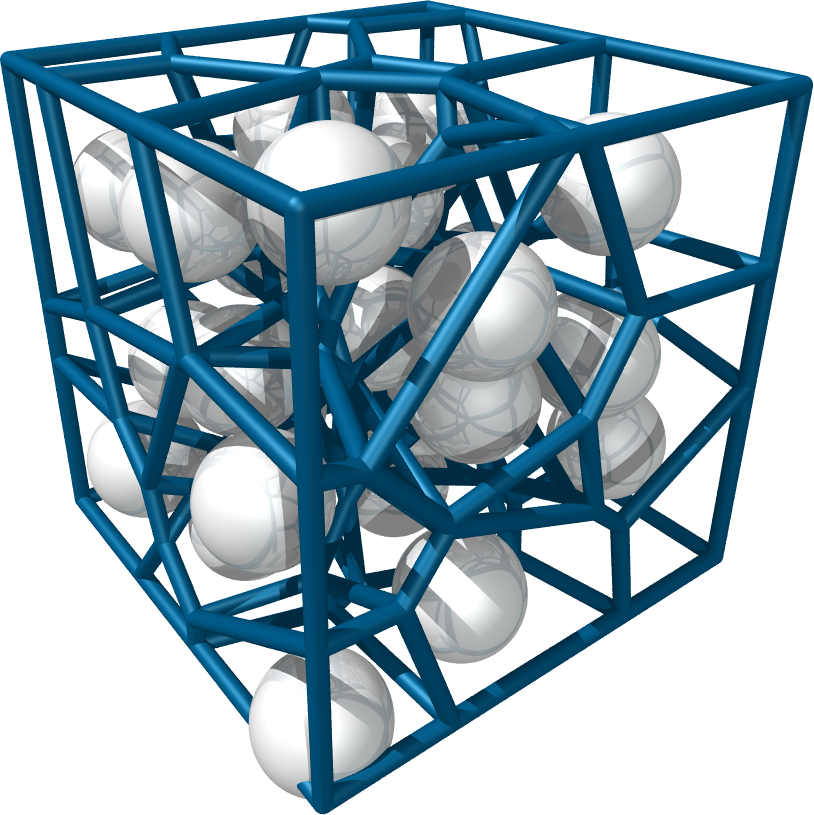
\includegraphics[width=0.8\textwidth]{images/voronoi/3d_diagram04_crop.png}%
        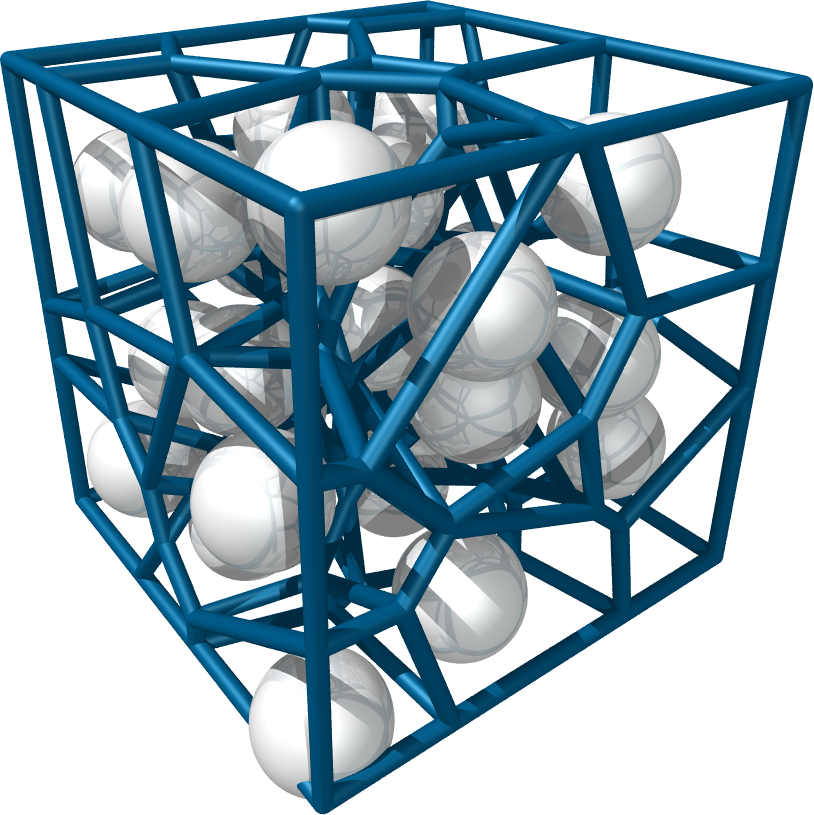
\includegraphics[height=0.7\textwidth]{images/voronoi/3d_diagram04_crop.png}%
        \caption{%
            Rendering of Voronoi cells in 3 dimensions, in a system of 27 particles. Voronoi cells created using the \cpp-library \texttt{Voro++}\cite{rycroft2009voro,webvoro++}, and rendered using the program \texttt{povray}\cite{webpovray}. %
            \label{fig:3d_voronoi_diagram}%
        }%
    \end{minipage}%
\end{figure}%

\todob{Something about removing hydrogen atoms, and just use oxygen position as hydrogen position, and water atom ``volume''? This simplifies life for us, since we don't have to find which water molecule each hydrogen atom belongs to, but we could get inconsistent water density. But since we use the same method for all measurements, we can compare relative densities.}

\todob{Something about removing extreme points/tail in distribution? Caused by vacuum.}

\section{Diffusion}
\todob{derivation of diffusion? See \cite[Section~4.4.1]{frenkel2001understanding}}
When we talk about diffusion in \hl{the context of} this thesis we mean the process of \emph{self-diffusion}, which is different from \hl{``normal''} diffusion which is the net movement of a substance in the presence of a gradient, which can be for example a concentration gradient, a temperature gradient, or a pressure gradient. With \emph{self-diffusion} we mean the \hl{random?} movement in a substance that has no gradients.

Diffusion can be characterized by a constant $D$, which is related to the displacement of each atom relative to a initial position. We can measure this constant by measuring the mean square displacement $r_i^2(t)$ of each atom as a function of time, and average over all atoms. The mean square displacement is measured as
\begin{align*}
    \Braket{r^2(t)} = \frac{1}{N} \sum_{i=1}^N \left( \rvec_i(t) - \rvec_i(t=0) \right)^2,
\end{align*}
where $\rvec_i(t=0)$ is the initial position of atom $i$. From theoretical considerations of the diffusion process we can relate the diffusion constant to the mean square displacement through\cite[Section~4.4.1]{frenkel2001understanding}
\begin{align}
    \lim_{t\rightarrow \infty}\dpd{}{t}\Braket{r^2(t)} = 2dD\label{eq:diffusion_derivative}
\end{align}
where $d$ is the \hl{spatial} \hl{dimensionality/dimension?}. This means that we can find the diffusion constant in a molecular dynamics simulation by measuring the mean square displacement for many timesteps, and find the slope of this data as the diffusion constant in the limit $t\rightarrow \infty$. \hl{We are limited in that we can't actually simulate infinite number of timesteps, but have to find a reasonable number of timesteps to measure over.} An example of how to sample the mean square displacement $\Braket{r^2(t)}$ in a simulation can be seen in \cref{list:diffusionSample}.
%
% This means that we can find the diffusion constant in a molecular dynamics simulation by measuring the mean square displacement for many timesteps, and plotting $\Braket{r^2(t)}/(2dt)$ as a function of time. The diffusion constant will then be the value this expression approaches when simulating for enough timesteps.
%
%An example of how to measure the mean square displacement in a molecular dynamics \hl{simulation/program} as outlined in \cref{chap:simple_md_program} can be seen in \cref{list:diffusionSample}.
% Fick's law relates flux $\bvec j$ of diffusing species to the concentration gradient $\bvec \nabla c$ of the species
% \begin{align*}
%     \bvec j = -D\bvec \nabla c,
% \end{align*}
% where $D$ is the proportionality constant called the diffusion \hl{coefficient/constant}.
% 
% Conservation of \hl{species/atoms?}
% \begin{align*}
%     \dpd{c(r,t)}{t} + \div \cdot \vec j(r,t) = 0,
% \end{align*}
% which gives
% \begin{align}
%     \dpd{c(r,t)}{t} - D\nabla^2 c(r,t) = 0.
%     \label{eq:diffusion_diff}
% \end{align}
% % We can solve this equation with the boundary condition
% % \begin{align*}
% %     c(r,0) = \delta (r),
% % \end{align*}
% % where $\delta(r)$ is the Dirac delta function, which gives
% % \begin{align*}
% %     c(r,t) = \frac{1}{(4\pi Dt)^{d/2}} \exp\left(-\frac{r^2}{4Dt}\right).
% % \end{align*}
% By multiplying \cref{eq:diffusion_diff} by $r^2$ and integrating over all space we get
% \begin{align*}
%     \dpd{}{t}\int \drvec~ r^2 c(r,t) = D\int \drvec~ r^2 \nabla^2 c(r,t).
% \end{align*}
% We recognize the integral on the left-hand side as the the mean square displacement %\hl{time dependence of the second moment of $c(r,t)$???}
% \todo{what???}
% \begin{align*}
%     \int \drvec~ c(r,t) r^2 \equiv \Braket{r^2(t)},
% \end{align*}
% where we have imposed
% \begin{align*}
%     \int \drvec~ c(r,t) = 1.
% \end{align*}
% Applying partial integration to the right-hand side we obtain
% \begin{align*}
%     \dpd{\Braket{r^2(t)}}{t} 
%     &= D\int \drvec~ r^2 \nabla^2 c(r,t) \\
%     &= D\int \drvec~ \div \cdot \left(r^2\nabla c(r,t)\right) - D\int\drvec~ \div r^2 \cdot \nabla c(r,t) \\
%     &= D\int \dif \vec S~ \left(r^2\div c(r,t)\right) - 2D\int\drvec~ \rvec \cdot\div c(r,t) \\
%     &= 0 - 2D\int\drvec~ (\div \cdot \rvec c(r,t)) + 2D\int\drvec~ (\div \cdot \rvec) c(r,t) \\
%     &= 0 + 2dD\int \drvec~ c(r,t) \\
%     &= 2dD
% \end{align*}
% 
% 
% \begin{align*}
%     \dpd{\Braket{r^2(t)}}{t} = 6D
% \end{align*}
% $\Rightarrow$ Plot mean square distance as function of time
% \begin{align*}
%     \Braket{\delta r(t)^2} = \frac{1}{N} \sum_{i=1}^N \delta \rvec_i(t)^2
% \end{align*}
% and find $6D$ as slope of plot \hl{(after a while?)}
%
\begin{listing}[!htb]%
\begin{cppcode*}{gobble=4}
    double diffusionSample(System &system)
    {
        double rSquared = 0.0;
        for (Atom *atom : system.atoms())
        {
            drVec = atom->positiom() - atom->initialPosition() 
                    + atom->getBoundaryCrossings()*system.size();
            rSquared += drVec.lengthSquared();
        }
        rSquared /= system.nAtoms();
        return rSquared;
    }
\end{cppcode*}
\caption{%
    An example of how to calculate the mean square displacement in a molecular dynamics simulation. Example implementation of \texttt{diffusionSample} from \cref{list:sampling}. We store the inital positions of the atoms as \texttt{atom->initialPosition()}, and when using periodic boundary conditions we count the number of times we have to translate the atom one system-size in each direction, so while the position of the atom will always be inside the system, the \hl{\emph{real}} position of the atom can be calculated by adding \texttt{atom->getBoundaryCrossings()*system.size()} to $\rvec$.%
    \label{list:diffusionSample}%
}%
\end{listing}%

% To improve our statistics when measuring the diffusion constant as function of distance to the surface of the pore we can use different time origins to get different samples. %
To measure $D$ we see from \cref{eq:diffusion_derivative} that we have to let $t\rightarrow \infty$, but in practice we see that the gradient of $\Braket{r^2(t)}$ usually stabilizes near its final value after ${\sim} 2\text{ k}$ timesteps. We can use this to get more samples for our measurements, by using different time origos. This means that when we have saved a number of states at \todoao{Finish diffusion time origo stuff}

% \FloatBarrier
\section{Tetrahedral order parameter}
The tetrahedral order parameter\cite{errington2001relationship} is effectively a measure of how tetrahedral a \hl{molecule?} is. The tetrahedral order parameter $Q$ for a molecule $k$ is calculated as follows
\begin{align*}
    Q_k = 1 - \frac{3}{8}\sum_i^3\sum_{j=i+1}^4 \left[ \cos \theta_{ikj} + \frac{1}{3} \right]^2,
\end{align*}
where $\theta_{ikj}$ is the angle between two vectors from the main molecule, $k$, to respectively atom $i$ and atom $j$, and the two sums go over the 6 possible angles $\theta_{ikj}$, between the main molecule and \hl{its} four nearest neighbors. See \cref{fig:top_tetrahedra} for an illustration of the angles and molecules involved in the calculation.
%
\begin{figure}[htpb]%
    \centering%
    \includesvg[width=0.3\textwidth, svgpath=./images/tetrahedral_order_parameter/]{tetrahedra02}%
    \caption{%
        Illustration of the angles and molecules involved in the calculation of the tetrahedral order parameter. The \hl{blue} dots are molecules, in our case usually water molecules. We have the center molecule $k$, and \hl{its} four nearest neighbors. $\theta_{ikj}$ is the angle between molecule $i$, $k$ and $j$, as indicated by the \hl{orange} arc. \hl{FINISH CAPTION}. %
        \label{fig:top_tetrahedra}%
    }%
\end{figure}%

% \FloatBarrier
\section{``Distance to atom''\label{sec:distance_to_atom}}
To help visualize, and to characterize our nanoporous system we developed a program that creates a 3d map of the distance to the nearest atom, in each point in space on a regular grid. The implementation of this program is almost straighforward, but since we have to do a lot of calculations if we want to have a map with decent resolution, we have also parallellized the program. 
\todoa{Write about distance to atom}
\todoc{Distance to atom code example?}

% \FloatBarrier
\section{``Generation matrix''}
Since the program from \cref{sec:distance_to_atom} takes a long time to run to get decent maps with high resolution, we decided to also develop a similar program that creates a 3d map of the space. To ease calculation we this time used a method inspired by the voxelation technique from \cref{sec:voxelation}. This program first divides the system into $n_x\times n_y\times n_z$ voxels, and make a 3d matrix of the same size for storing the label of each voxel. We first give all voxels with one or more atoms in them the label \hl{``0''}. We then label the rest of the voxels using an iterative method, increasing the \hl{numbers/labels} for each iteration. In each iteration we find the voxels that have a neighbor voxel \hl{labelled} with the previous label (\texttt{label-1}), using 4-neighbor connectivity, and give them the current label. When all voxels are labelled, they should have a label corresponding to the \hl{Manhattan distance} to the nearest atom.

Although the Manhattan distance isn't as useful as the regular Euclidean distance we calculate using the \hl{``distance to atom''}-program, the benefit is that making a 3d map of space using the \hl{``generation matrix''} method uses about 3\% of the time that ``distance to atom'' uses for the same system and same resolution. 

\todoa{Something about the usefulness of this measure?}

\orangebox{A system of 347176 atoms (\texttt{rough\_fracture03}), water and SiO2, $256^3$ voxels, $~5$ seconds for ``generation matrix'', 2m27seconds for ``distance to atom'' (on one cpu)}
\todoc{Voxel counter code example?}

% \FloatBarrier
\section{``Voxel counter''}
\todob{Write about voxel counter}
\todod{Voxel counter code example?}
    A histogram of the fraction of voxels that has one or more atom in them vs. the voxel size in x-, y-, and z-direction.
    
% \FloatBarrier
\section{Cage cage correlation}
    \todod{Measure cage cage correlation}

% \FloatBarrier
\section{Surface area of pores}
    Only one large pore in my system, so not useful?

    \chapter{Studied systems}
% \todoa{Write about the systems we studied}%
% \todoa{Rename flat fracture systems to reference?}
% \todoa{Write about density and vacuum problems - injected water with high density in some systems - SEPARATE (sub)SECTION?}
%
% flat_square_fracture02
% flat_square_fracture03
% flat_fracture02
% flat_fracture03
% rough_fracture01_abel
% rough_fracture03
% rough_fracture04_same_distance
% rough_fracture05
%
We have do experiments on a total of 8 different systems, all consisting of a slab of silica with a fracture in the center filled with water. Four of them are ``reference'' systems with just a flat fracture in the center, and the other four are systems with a random fracture with different geometries.

All systems are created using the experimental procedure from \cref{sec:experimental_procedure}. The systems are initialized as a perfect crystal of $\upbeta$-cristobalite. The system is then brought to 4500 Kelvin using a thermostat, to melt the silica crystal. It is then cooled back down to 300 Kelvin, and a fracture is cut out of the solid slab of silica, the system dangling ends are passivated, and the fracture is filled with water. The system is then thermalized at 300 Kelvin.

A summary of the different systems can be seen in \cref{tab:systems}, where we have listed the dimension, porosity, the number of atoms, and the number of SiO$_2$ and water \hl{units/species} in each system.
%
\begin{table}[htpb]
\centering
    \begin{tabular}{l|cccccc}
    \textit{System}             & \textit{Dimensions} [\AA]     & $\phi$ [\%]   & \textit{r} [\AA]  & $N$       & $N_\text{SiO$_2$}$    & $N_\text{H$_2$O}$ \\ \hline 
    Rough fracture \#1          & $179 \times 179 \times 179$   & ${\sim}12$    & -                 & 393 k  & 111 k                    & 19 k           \\ % rough_fracture01_abel, N = 393181
    Rough fracture \#2          & $172 \times 172 \times 172$   & ${\sim}13$    & -                 & 347 k  & 97 k                     & 18 k            \\ %rough_fracture03, N = 347176
    Rough fracture \#3          & $172 \times 172 \times 172$   & ${\sim}13$    & 14.4              & 349 k  & 99 k                     & 16 k            \\ % rough_fracture04_same_distance, N = 348573
    Rough fracture \#4          & $172 \times 172 \times 172$   & ${\sim}23$    & 28.8              & 368 k  & 89 k                     & 34 k            \\ % rough_fracture05 N = 367958
    \hline %
    Reference \#1           & $179 \times 179 \times 179$   & 48            & 86                & 260 k     & 25 k                  & 60 k                             \\ % flat_square_fracture02, N = 259955
    Reference \#2           & $179 \times 179 \times 179$   & 48            & 86                & 271 k     & 25 k                  & 64 k                             \\ % flat_square_fracture03, N = 271328
    Reference \#3           & $143 \times 143 \times 57$    & 25            & 14.4              & 90 k      & 19 k                  & 10 k                             \\ % flat_fracture02, N = 89646
    Reference \#4           & $143 \times 143 \times 57$    & 50            & 28.8              & 107 k     & 13 k                  & 22 k                             \\ % flat_fracture03, N = 106829
    \end{tabular}%
    \vspace{8pt}
    \caption{%
%     \caption{%
%     a
        An overview of the 8 different systems we have done experiments on. ``Flat fracture'' 1 through 4 are reference systems, that consist of a silica slab with a single flat fracture filled with water. ``Rough fracture'' 1 through 4 consist of a silica slab with different water-filled fractures with different geometries.%
        \\%
%
        $\phi$ is the approximate porosity of the system, defined as the volume of the fracture relative to the volume of the whole system. $r$ is the distance between the surfaces used to create the fracture. $N$ is the total number of atoms (silicon, oxygen and hydrogen), $N_\text{SiO$_2$}$ is the number of SiO$_2$-units, and $N_\text{H$_2$O}$ is the number of water molecules. %
%
%         $N_\text{H$_2$O}$ and $N_\text{SiO$_2$}$ measured in flat02 and flat03 using slice of heigth 14.4/28.8, and then counting number of oxygen/silicon in slice. \hl{Volumes of rough fractures calculated using Ovito ``construct surface mesh''}%
        \label{tab:systems}%
%     }%
    }
\end{table}%

In all systems with narrow pores and fractures we noticed that the water filling method had some problems. This is caused by the voxelation method used to fill the system, where we divide the system into voxels, mark all voxels with atoms in them (before filling the system with water) as occupied, and then put one water molecule in each unoccupied voxel. When marking occupied voxels we usually end up marking a lot of the voxels at the silica surface as occupied. This means that when we have very narrow pores, with the distance between the pore walls in the same range as the voxel size, a large fraction of the pore will be occupied voxels, and the resulting water density in the pore will be lower than the expected density. To rectify this we use higher input densities when filling narrow fractures and pores with water.


\subsection*{Rough fractures}
The fractures in the systems labelled ``rough fracture'' are all created using periodic surfaces with a Hurst exponent close to \hl{0.75}, generated using successive random additions from \cref{sec:diamond_square_2d_finite}, and the fractures cut out using the method from \cref{sec:generating_fractures}. ``Rough fracture'' \#1 and \#2 are created using different surfaces for the top and bottom of the fracture, while ``rough fracture'' \#3 and \#4 are created using the same surface repeated twice for the top and bottom of the fracture, with a distance of respectively 14.4 and 28.8 \AA\ between the surfaces, which gives an approximately constant width fracture. 

When filling system \#1 and \#2 with water we used an input density of 1050 kg/m$^3$, and for system \#3 and \#4 we used 1273 kg/m$^3$.

% When filling the narrow fractures in ``rough fracture'' \#3 and \#4 the water filling method had a lot of trouble, since the pore size is very close to the voxel size it ends up using. This means that a lot of the voxels in the pore end up being unavailable for putting water atoms in, and the net water density we end up with is usually much lower than the input density. We solve this by increasing the input density until the system seems somewhat saturated (using visual inspection, and looking at density profiles).

\subsection*{Reference systems}
To compare with the fracture systems we have also prepared four ``reference'' systems, all consisting of one flat pore with constant width. 

``Reference'' \#1 and \#2 both have a 86 \AA\ wide pore. When filling system \#1 and \#2 with water we used an input density of respectively 1050 and 1126 kg/m$^3$%
%, which, as we will see, resulted in bulk densities of respectively 1038 and 1126 kg/m$^3$ (see \cref{tab:bulk_water_density})%
. These two systems will serve as good references for the behaviour and structure of water near the silica surface, and in bulk-like conditions, as we expect the water in the middle of the pore to display bulk-like behaviour.%\todoao{Write more about increased density and vacuum, maybe in discussion/conclusion?}
%
% . After thermalizing this system we noticed some vacuum bubbles in the water near the silica surface, so in system \#2 we tried using a higher density when filling the pore with water, and we ended up using an input density of 1126 kg/m$^3$, which resulted in a bulk density of 1090 (see \cref{tab:bulk_water_density}). From phase diagrams of water \todobo{cite?} we know that water has the same phase in a wide range of densities and pressures, so we do not risk drastically changing the behaviour of the water atoms by increasing the density to 1090 kg/m$^3$.%
%

``Reference'' \#3 and \#4 consist of flat pores that are respectively 14.4 and 28.8 \AA\ wide, which we will compare to the random fracture systems with random uniform fractures in them. When filling the pores in these systems with water we used input densities of 1273 kg/m$^3$. This is a pretty high density, but the voxelation method had some problems in very narrow fractures, giving a lower density than intended, which made us use a higher density to reach an approximate density of 1000 kg/m$^3$.
%when the pore sizes are in the same range as the voxel size, which makes the resulting density a lot lower than the input density. We also had problems with vacuum bubbles near the silica surface in these two systems, but this was somewhat remedied by increasing the water density. \todoao{Write about problems with injecting water in narrow fractures and pores}
    \chapter{Re}
\section{Density}
\begin{figure}[htpb]%
    \centering%
    \includesvg[width=0.7\textwidth, svgpath=./images/density/]{density_water02}%
    \caption{%
        Density of water. \hl{FINISH CAPTION}. %
%         \label{fig:cell_lists}%
    }%
\end{figure}%
\begin{figure}[htpb]%
    \centering%
    \includesvg[width=0.7\textwidth, svgpath=./images/density/]{number_of_molecules02}%
    \caption{%
        Number of molecules. Bin width = 0.2 \AA?. \hl{FINISH CAPTION}. %
%         \label{fig:cell_lists}%
    }%
\end{figure}%

\FloatBarrier
\section{Diffusion/mean square displacement}
\todo[inline]{Diffusion normal to and parallel to surface?}
\begin{figure}[htpb]%
    \centering%
    {
        \newcommand{\f}{\footnotesize}
        \includesvg[width=0.7\textwidth, svgpath=./images/diffusion/]{diffusion01}%
    }
    \caption{%
        Diffusion. \hl{FINISH CAPTION}. %
%         \label{fig:cell_lists}%
    }%
\end{figure}%

\begin{figure}[htpb]%
    \centering%
    {
        \newcommand{\f}{\footnotesize}%
        \includesvg[width=0.7\textwidth, svgpath=./images/diffusion/]{diffusion_constant02}%
    }
    \caption{%
        Diffusion. \hl{Consider fixing label background...} \hl{FINISH CAPTION}. %
%         \label{fig:cell_lists}%
    }%
\end{figure}%

\FloatBarrier
\section{Distance to atom}
\todo{replace these with results from actual fracture system?}
We developed a program that finds the distance to the nearest atom, in all points of the 
%
\setlength{\myfigwidth}{0.90\textwidth}%
\begin{figure}[htpb]%
    \centering%
    \includesvg[width=\myfigwidth, svgpath = ./images/distance_to_atom/]{SiO2_06_slice_r05_n256}%
    \caption{$r = 5$ \Ang}%
    \label{fig:distance_to_atom_r05}%
\end{figure}%
%
\begin{figure}[htpb]%
    \centering%
    \includesvg[width=\myfigwidth, svgpath = ./images/distance_to_atom/]{SiO2_06_slice_r20_n256}%
    \caption{$r = 20$ \Ang}%
    \label{fig:distance_to_atom_r20}%
\end{figure}%

\FloatBarrier
\section{``Generation matrix''}
\todo{replace these with results from actual fracture system?}
Not very useful. Much of the same as distance to atom, only worse (but faster).
%
\begin{figure}[htpb]%
    \centering%
    \includesvg[width=\myfigwidth, svgpath = ./images/generation_matrix/]{SiO2_06_slice_r05_n256}%
    \caption{5 generations}%
    \label{fig:generation_matrix_r05}%
\end{figure}%
%
\begin{figure}[htpb]%
    \centering%
    \includesvg[width=\myfigwidth, svgpath = ./images/generation_matrix/]{SiO2_06_slice_r11_n256}%
    \caption{11 generations}%
    \label{fig:generation_matrix_r11}%
\end{figure}%
%
\begin{figure}[htpb]%
    \centering%
    \includesvg[width=\myfigwidth, svgpath = ./images/generation_matrix/]{SiO2_06_slice_r40_n256}%
    \caption{40 generations}%
    \label{fig:generation_matrix_r40}%
\end{figure}%

\FloatBarrier
\section{Tetrahedral order parameter}


% \setlength{\myfigwidth}{0.499\textwidth}%
% \begin{figure}[htpb]%
%     \centering%
%     \begin{subfigure}[b]{\myfigwidth}%
%         \includesvg[width=\textwidth, svgpath=./images/tetrahedral_order_parameter/]{figure04}%
%         \caption{Caption}%
% %         \label{fig:pass_tet01}%
%     \end{subfigure}%
% %     \hspace{0.05\textwidth}%
%     \begin{subfigure}[b]{\myfigwidth}%
%         \includesvg[width=\textwidth, svgpath=./images/tetrahedral_order_parameter/]{figure07}%
%         \caption{Caption}%
% %         \label{fig:pass_tet02}%
%     \end{subfigure}%
%     
%     \begin{subfigure}[b]{\myfigwidth}%
%         \includesvg[width=\textwidth, svgpath=./images/tetrahedral_order_parameter/]{figure09}%
%         \caption{Caption}%
% %         \label{fig:pass_tet02}%
%     \end{subfigure}%
%     \begin{subfigure}[b]{\myfigwidth}%
%         \includesvg[width=\textwidth, svgpath=./images/tetrahedral_order_parameter/]{figure10}%
%         \caption{Caption}%
% %         \label{fig:pass_tet02}%
%     \end{subfigure}%
%     
%     \begin{subfigure}[b]{\myfigwidth}%
%         \includesvg[width=\textwidth, svgpath=./images/tetrahedral_order_parameter/]{figure11}%
%         \caption{Caption}%
% %         \label{fig:pass_tet02}%
%     \end{subfigure}%
%     \begin{subfigure}[b]{\myfigwidth}%
%         \includesvg[width=\textwidth, svgpath=./images/tetrahedral_order_parameter/]{figure12}%
%         \caption{Caption}%
% %         \label{fig:pass_tet02}%
%     \end{subfigure}%
%     %
%     \caption{%
%         \hl{Caption}%
%     }%
% %     \label{fig:inject_empty_voxel}%
% \end{figure}%

%
\begin{figure}[htpb]%
    \centering%
    \includesvg[width=1.0\textwidth, svgpath = ./images/tetrahedral_order_parameter/]{fancyfig04}%
    \caption{}%
%     \label{fig:distance_to_atom_r20}%
\end{figure}%

\FloatBarrier
\section{Area}
\section{Volume?}



\part{Conclusion}
    \chapter{Conclusion}
- small differences between flat and rough, and between the two rough types, but clear trends in water transport properties and structure (diff, TOP) near surface
- density 8-10 ang, diffusion and TOP 5-6 ang

important with density control in future experiments - new methods (use tetrahedra?)

\chapter{Future}
Measure in narrower fracture -- hard to initialize -- new inject methods
Better method for creating uniform width fractures? Since our method only creates equal $\Delta z$
    \chapter{Future}

\part{Appendices}
\begin{appendix}
%     \chapter{Reduced units/MD units}
 % remove md units completely?
    \chapter{Verlet integrators\label{appendix:verlet_integrators}}

\fcolorbox{black}{orange}{
\begin{minipage}{\textwidth}
{\bf TODO:}
\begin{itemize}
    \item Truncation error Verlet/velociy Verlet
    \item Numerical stability?
    \item Memory?
    \item Self starting, symplectic, reversible
\end{itemize}
\end{minipage}
}
\todo{why do we use velocity Verlet}

The Verlet algorithm\cite{verlet1967computer} is a simple method for \hl{numerically?} integrating second order differential equations of the form 
\begin{align*}
    \dod[2]{\rvec(t)}{t} = \Fvec\big[\rvec(t), t\big] = \Fvec(t).
\end{align*}
The algorithm has several \hl{(equivalent?)} forms, and the form \hl{used/developed?} by Verlet is
\begin{align*}
    \rvec(t + \Delta t) \approx 2\rvec(t) - \rvec(t - \Delta t) + \avec(t)\Delta t^2,
\end{align*}
where $\Delta t$ is the timestep\todo{define timestep}, and $\avec(t)$ is the velocity at time $t$. An equivalent formulation, usually called the velocity Verlet algorithm, has the form
\begin{align*}
    \rvec(t + \Delta t) &= \rvec(t) + \vvec(t)\Delta t + \frac{\Fvec(t)}{2m}\Delta t^2 \\
    \vvec(t + \Delta t) &= \vvec(t) + \frac{\Fvec(t + \Delta t) + \Fvec(t)}{2m}\Delta t.
\end{align*}
The velocity Verlet algorithm is the most used form \hl{why?}, and \hl{something about errors, references to below}.

This algorithm has a \hl{glocal/accumulated} error of $\mathcal{O}(\Delta t^2)$\todo{either \cite{thijssen1999computational} sec. 8.4.1-8.4.3 or \cite{frenkel2001understanding} sec. 4.3.3}.

% \section{Verlet integrators}
% \begin{align*}
%     \rvec(t) = r_n \\
%     \vvec(t) = v_n \\
%     \bvec a(t) = a_n.
% \end{align*}
% \begin{align*}
%     \vvec_{n+1/2} = \vvec_n + \frac{1}{2}\bvec a_n \delta t \\
%     \rvec_{n+1} = \rvec_n + \vvec_{n+\frac{1}{2}}\delta t
% \end{align*}

% \begin{align*}
%     \vvec(t + \Delta t/2) &= \vvec(t) + \frac{1}{2}\bvec a(t) \Delta t \\
%     \rvec(t + \Delta t)   &= \rvec(t) + \vvec(t + \Delta t/2)\Delta t \\
%     \bvec a(t + \Delta t)   &= \frac{1}{m}\Fvec(\rvec(t + \Delta t)) \\
%     \vvec(t + \Delta t)   &= \vvec(t + \Delta t) + \frac{1}{2}\bvec a(t + \Delta t) \Delta t
% \end{align*}

We will now first derive the regular Verlet and the velocity Verlet algorithms using Taylor expansions, and then using the Liouville formulation of classical mechanics. \todo{why use two methods? what do we learn from them?} \todo{mention what errors we find?}

\section{Deriving the Verlet algorithm using Taylor expansions\label{appendix:verlet_taylor}}

To derive the algorithm we first let
\begin{align*}
    \dod{\rvec(t)}{t} &= \vvec(t),
\end{align*}
and
\begin{align*}
    \dod{\vvec(t)}{t} &= \avec(t) = \frac{\Fvec(t)}{m}.
\end{align*}

We then do a Taylor expansion of $\rvec(t \pm \Delta t)$ around time $t$
\begin{align}
    \rvec(t + \Delta t) &= \rvec(t) + \vvec(t)\Delta t + \avec(t)\frac{\Delta t^2}{2} + \dod[3]{\rvec(0)}{t}\frac{\Delta t^3}{6} + \mathcal{O}(\Delta t^4), \label{eq:verlet_plus}\\
    \rvec(t - \Delta t) &= \rvec(t) - \vvec(t)\Delta t + \avec(t)\frac{\Delta t^2}{2} - \dod[3]{\rvec(0)}{t}\frac{\Delta t^3}{6} + \mathcal{O}(\Delta t^4).\label{eq:verlet_minus}
\end{align}
By summing these two equations we get
\begin{align*}
    \rvec(t + \Delta t) + \rvec(t - \Delta t) = 2\rvec(t) + \avec(t)\Delta t^2 + \mathcal{O}(\Delta t^4),
\end{align*}
which by rearranging can be written as
\begin{align*}
    \rvec(t + \Delta t) \approx 2\rvec(t) - \rvec(t - \Delta t) + \avec(t)\Delta t^2.
\end{align*}
This is the equation used to update the positions in the regular Verlet algorithm. We see that the estimate of the new position contains an truncation error for one timestep $\Delta t$ of the order $\mathcal{O}(\Delta t^4)$.

The Verlet algorithm does not use the velocity to compute the new position, but we can find an estimate of the velocity by taking the difference between \cref{eq:verlet_plus,eq:verlet_minus}
\begin{align*}
    \rvec(t + \Delta t) - \rvec(t - \Delta t) = 2\vvec(t)\Delta t + \mathcal{O}(\Delta t^3),
\end{align*}
which by rearranging can be written as
\begin{align*}
    \vvec(t) = \frac{\rvec(t + \Delta t) - \rvec(t - \Delta t)}{2\Delta t} + \mathcal{O}(\Delta t^2).
\end{align*}
We see that this estimate of the velocity has a truncation error of the order $\mathcal{O}(\Delta t^2)$, compared to the error in the position $\mathcal{O}(\Delta t^4)$.
\todo{Something about lower precision}

\subsection{Velocity Verlet}
A modification of the Verlet algorithm usually called the velocity Verlet algorithm\cite{swope1982computer} \todo{something about why velocity Verlet is good} can be derived in a similar way. We have the same Taylor expansion of $\rvec(t+\Delta t)$ around $t$ as before
\begin{align}
    \rvec(t + \Delta t) &= \rvec(t) + \vvec(t)\Delta t + \avec(t)\frac{\Delta t^2}{2} + \mathcal{O}(\Delta t^3), \label{eq:position_taylor}
\end{align}
and now we also expand $\vvec(t + \Delta t)$ around $t$
\begin{align}
    \vvec(t + \Delta t) 
%     &= \vvec(t) + \dod{\vvec(t)}{t}\Delta t + \dod[2]{\vvec(t)}{t}\frac{\Delta t^2}{t} + \mathcal{O}(\Delta t^3) \\
    &= \vvec(t) + \avec(t)\Delta t + \dod[2]{\vvec(t)}{t}\frac{\Delta t^2}{2} + \mathcal{O}(\Delta t^3). \label{eq:velocity_taylor}
\end{align}
We now need an expression for $\od[2]{\vvec(t)}{t}$, which can be found by a Taylor expansion of $\od{\vvec(t+\Delta t)}{t}$
\begin{align*}
    \dod{\vvec(t+\Delta t)}{t} = \dod{\vvec(t)}{t} + \dod[2]{\vvec(t)}{t}\Delta t + \mathcal{O}(\Delta t^2),
\end{align*}
which by rearranging and multiplying with $\frac{\Delta t}{2}$ gives
\begin{align*}
    \dod[2]{\vvec}{t}\frac{\Delta t^2}{2} 
    &= \left( \dod{\vvec(t+\Delta t)}{t} - \dod{\vvec(t)}{t}\right)\frac{\Delta t}{2} + \mathcal{O}(\Delta t^3) \\
    &= \big[\avec(t + \Delta t) - \avec(t)\big] \frac{\Delta t}{2} + \mathcal{O}(\Delta t^3).
\end{align*}
Inserting this into \cref{eq:velocity_taylor} we get
\begin{align}
    \vvec(t + \Delta t) 
    &= \vvec(t) + \avec(t)\Delta t + \big[\avec(t + \Delta t) - \avec(t)\big] \frac{\Delta t}{2} + \mathcal{O}(\Delta t^3) \nonumber\\
    &= \vvec(t) + \big[\avec(t) + \avec(t + \Delta t)\big] \frac{\Delta t}{2} + \mathcal{O}(\Delta t^3). \label{eq:verlet_velocity_taylor_insertion}
\end{align}
So the total velocity Verlet algorithm with truncation of the higher-order terms is
\begin{align}
    \rvec(t + \Delta t) &= \rvec(t) + \vvec(t)\Delta t + \avec(t)\frac{\Delta t^2}{2} %\label{eq:velocity_verlet_position}
    \\
    \vvec(t + \Delta t) &= \vvec(t) + \big[\avec(t) + \avec(t + \Delta t)\big] \frac{\Delta t}{2}, %\label{eq:velocity_verlet_velocity}
\end{align}
with the truncation error for one timestep $\Delta t$ being of the order $\mathcal{O}(\Delta t^3)$ for both the position and the velocity. 

% \subsection{Implementation}
% \todo{Remove this subsec? Included in MD part}
% The algorithm is usually rewritten in the following way, to optimize the implementation on a computer. We see that the new velocities can be written as
% \begin{align}
%     \vvec(t+\Delta t) = \tilde\vvec(t + \tfrac{1}{2}\Delta t) + \avec(t+\Delta t)\frac{\Delta t}{2}, %\label{eq:verlet_velocity_with_halfstep}
% \end{align}
% where
% \begin{align}
%     \tilde\vvec(t + \tfrac{1}{2}\Delta t) = \vvec(t) + \avec(t)\frac{\Delta t}{2}. \label{eq:verlet_halfstep}
% \end{align}
% We see that \cref{eq:verlet_halfstep} can be used in updating the positions, so we rewrite \cref{eq:velocity_verlet_position} to
% \begin{align}
%     \rvec(t + \Delta t) &= \rvec(t) + \tilde\vvec(t+\tfrac{1}{2}\Delta t)\Delta t. %\label{eq:velocity_verlet_positions_halfstep}
% \end{align}
% Which leads us to the usual way of implementing the algorithm\cite{allen1989computer}:
% \begin{itemize}
%     \item Calculate the velocities at $t+\tfrac{1}{2}\Delta t$ using \cref{eq:verlet_halfstep} \hl{(repeated here)}
%     \begin{align*}
%         \tilde\vvec(t + \tfrac{1}{2}\Delta t) = \vvec(t) + \frac{\Fvec(t)}{m}\frac{\Delta t}{2}.
%     \end{align*}
%     \item Calculate the new positions at $t + \Delta t$ using \cref{eq:velocity_verlet_positions_halfstep} \hl{(repeated here)}
%     \begin{align*}
%         \rvec(t + \Delta t) &= \rvec(t) + \tilde\vvec(t+\tfrac{1}{2}\Delta t)\Delta t.
%     \end{align*}
%     \item Calculate the new forces $\Fvec(t+\Delta t)$.
%     \item Calculate the new velocities at $t+\Delta t$ using \cref{eq:verlet_velocity_with_halfstep} \hl{(repeated here)}
%     \begin{align*}
%         \vvec(t+\Delta t) = \vvec(t + \tfrac{1}{2}\Delta t) + \frac{\Fvec(t + \Delta t)}{m}\frac{\Delta t}{2}.
%     \end{align*}
% \end{itemize}
% This implementation minimizes the memory needs, as we only need to store one copy of $\rvec$, $\vvec$ and $\Fvec$ at all times, compared to implementing \cref{eq:velocity_verlet_position,eq:velocity_verlet_velocity} which needs to store the values of both $\Fvec(t)$ and $\Fvec(t+\Delta)$ to calculate the new velocities. 
% 
% Pseudocode: \todo{do we want this?}
% \begin{verbatim}
%     v += F*dt/(2*m);
%     r += v*dt;
%     F = calculate_forces(r, v);
%     v += F*dt/(2*m);
% \end{verbatim}



% The velocity Verlet algorithm can be implemented as follows\cite{allen1989computer}
% \begin{samepage}
% \begin{itemize}
%     \item Calculate the new positions at $t + \Delta t$ using \cref{eq:velocity_verlet_position}.
%     \item Calculate the velocities at $t + \frac{1}{2}\Delta t$ using
%     \begin{align*}
%         \vvec(t + \tfrac{1}{2}\Delta t) = \vvec(t) + \frac{\Fvec(t)}{m}\frac{\Delta t}{2}.
%     \end{align*}
%     \item Calculate the new forces $\Fvec(t + \Delta t)$.
%     \item Finally, calculate the new velocities at $t + \Delta t$ using
%     \begin{align*}
%         \vvec(t + \Delta t) = \vvec(t + \tfrac{1}{2}\Delta t) + \frac{\Fvec(t + \Delta t)}{m}\frac{\Delta t}{2}
%     \end{align*}
% \end{itemize}
% \end{samepage}
% But 
% This implementation uses $9N$ units of memory, 

\section{Global error in the Verlet algorithm - BAD}
Sources:
\begin{itemize}
    \item \url{http://math.stackexchange.com/questions/668707/verlet-method-global-error}
    \item \url{http://www.saylor.org/site/wp-content/uploads/2011/06/MA221-6.1.pdf} (same as Wikipedia)
\end{itemize}

\todo{I don't know if the calculations below are correct} 
The global error in position can be derived from the local error for one timestep $\Delta t$. We see from \cref{eq:position_taylor} that
\begin{align*}
    \text{error}\big(\rvec(t_0+\Delta t)\big) = \mathcal{O}(\Delta t^3),
\end{align*}
and from \cref{eq:verlet_velocity_taylor_insertion}
\begin{align*}
    \text{error}\big(\vvec(t_0+\Delta t)\big) = \mathcal{O}(\Delta t^3).
\end{align*}
The error for two timesteps is
\begin{align*}
    \rvec(t_0+2\Delta t) 
    &= \rvec(t_0+\Delta t) + \vvec(t_0+\Delta t)\Delta t + \avec(t_0+\Delta t)\frac{\Delta t^2}{2} + \mathcal{O}(\Delta t^3), \\
\end{align*}
which gives \todo{Error in $\avec(t_0 + \Delta t) = \mathcal{O}(\Delta t^3)$ ??}
\begin{align*}
    &\text{error}\big(\rvec(t_0+2\Delta t)\big) \\
    &~= \text{error}\big(\rvec(t_0+\Delta t)\big) + \text{error}\big(\vvec(t_0+\Delta t)\big)\Delta t + \text{error}\big(\avec(t_0+\Delta t)\big)\frac{\Delta t^2}{2} + \mathcal{O}(\Delta t^3)\\
    &~= \mathcal{O}(\Delta t^3) + \mathcal{O}(\Delta t^3)\Delta t + \mathcal{O}(\Delta t^3)\frac{\Delta t^2}{2} + \mathcal{O}(\Delta t^3)\\
    &~= 2\mathcal{O}(\Delta t^3).
\end{align*}
Similarly we find
\begin{align*}
    &\text{error}\big(\rvec(t_0+3\Delta t)\big) = 3\mathcal{O}(\Delta t^3) \\
    &\text{error}\big(\rvec(t_0+4\Delta t)\big) = 4\mathcal{O}(\Delta t^3) \\
    &\text{error}\big(\rvec(t_0+5\Delta t)\big) = 5\mathcal{O}(\Delta t^3),
\end{align*}
\begin{align*}
    \text{error}\big(\rvec(t_0 + n\Delta t)\big) = n\mathcal{O}(\Delta t^3) = \mathcal{O}(\Delta t^2)
\end{align*}

\section{Deriving velocity Verlet using Liouville operator\label{sec:liou}\label{appendix:liouville_verlet}}
\newcommand{\Liou}{i\hat{\vec L}}
\newcommand{\Lop}{\hat{\mathcal{U}}}
% \todo{Cite Tuckerman et al. ([71] in Frenkel) ?}
%
We will now derive the velocity Verlet algorithm in a more rigorous way, using the Liouville formulation of classical mechanics. This approach will give us better insight into why the algorithm is so powerful, and a good estimate of the global (or accumulated) error of this algorithm. The derivation closely follows section 4.3.3 in \cite{frenkel2001understanding}.

\subsection{Liouville operator}
We have a system consisting of $N$ particles, with positions $\rvec$ and momenta $\vec p$. We define a function of these variables $f(\rvec(t), \vec p(t)) = f(t)$, that has the time derivative %
%(the derivative is denoted by a dot)
(denoted by a dot)
\begin{align}
    \dot f(t) = \dot \rvec \dpd{f(t)}{\rvec} + \dot {\vec p} \dpd{f(t)}{\vec p} = \Liou f(t).
    \label{eq:liou_f}
\end{align}
where we have defined the \emph{Liouville operator}, $\Liou$, as
\begin{align*}
    \Liou = \dot \rvec \dpd{}{\rvec} + \dot {\vec p} \dpd{}{\vec p} = \Liou_r + \Liou_p
\end{align*}
where $\Liou_r$ and $\Liou_p$ denotes the left and right part if this operator, respectively. %
We can formally integrate \cref{eq:liou_f} to obtain
\begin{align}
    f(t) = e^{\Liou t} f(0),
    \label{eq:liou_integrate}
\end{align}
which allows us to define the time evolution operator $\Lop = \exp(\Liou t)$. We see that this integration doesn't get us any closer to finding $f(t)$%\todo{why do we want to find $f(t)$?}%
, since evaluating the right-hand side is equivalent to the exact integration of the classical equations of motion. To get around this we define the time evolution operator for positions $\Lop_r(t) = \exp(\Liou_r t)$, and try applying just this operator. If we do a Taylor expansion of the exponential we get
\begin{align*}
    \Lop_r(t)f(0)
    &= f(0) + \Liou_r t f(0) + \frac{(\Liou_r t)^2}{2!} f(0) + \dots \\
    &= \exp\left( \dot\rvec (0) t \dpd{}{\rvec} \right) f(0) \\
    &= \sum_{n=0}^\infty \frac{ \big(\dot\rvec(0) t\big)^n}{n!} \frac{\partial^n}{\partial \rvec^n} f(0) \\
    &= f\left\{ \left[ \rvec(0) + \dot\rvec(0)t \right], \vec p(0) \right\},
\end{align*}
where $\rvec(0)$ and $\vec p(0)$ are the positions and momenta at $t = 0$. We see that this has the effect of moving the positions $\rvec$ a step $t$ forward in time according to their derivative. It's easy to see that the equivalent momentum time evolution operator $\Lop_p(t) = \exp(\Liou_p t)$ has a similar effect on the momenta. 

\subsection{Velocity Verlet}
In a molecular dynamics simulation we would like to be able to apply these operators independently, since
\begin{align*}
    \Lop = e^{\Liou} = e^{\Liou_r + \Liou_p},
\end{align*}
but unfortunately, for two noncommuting operators $\hat {\vec A}$ and $\hat {\vec B}$ we have
\begin{align*}
    e^{\hat {\vec A} + \hat {\vec B}} \neq e^{\hat {\vec A}} e^{\hat {\vec B}}.
\end{align*}
To solve this we can use the following \emph{Trotter identity}
\begin{align*}
    e^{\hat {\vec A} + \hat {\vec B}} = \lim_{P\rightarrow \infty} \left( e^{\hat {\vec A}/2P} e^{\hat {\vec B}/P} e^{\hat {\vec A}/2P} \right)^P.
\end{align*}
Applying the operators an infinite number of times ($P\rightarrow \infty$) is unpractical, but fortunately the expression can be truncated for large but finite $P$ as
\begin{align}
    e^{\hat {\vec A} + \hat {\vec B}} = \left( e^{\hat {\vec A}/2P} e^{\hat {\vec B}/P} e^{\hat {\vec A}/2P} \right)^P e^{\mathcal{O}(1/P^2)}.
    \label{eq:liou_time_exact}
\end{align}

To derive the velocity Verlet scheme using this truncation we first identify the operators $\hat {\vec A}$ and $\hat {\vec B}$ as
\begin{align*}
    \frac{\hat {\vec A}}{P} &\equiv \frac{\Liou_p t}{P} \equiv \Delta t \dot {\vec p}(0) \dpd{}{\vec p} \\
    \frac{\hat {\vec B}}{P} &\equiv \frac{\Liou_r t}{P} \equiv \Delta t \dot \rvec (0) \dpd{}{\rvec}
\end{align*}
where $\Delta t = t/P$. We can now identify the \emph{truncated} time evolution operator $\Lop^*(t)$ as follows
\begin{align}
    \Lop(t) 
    &= \left( e^{\Liou_p\Delta t/2} e^{\Liou_r \Delta t} e^{\Liou_p \Delta t/2} \right)^P e^{\mathcal{O}(1/P^2)} \nonumber\\
    &\approx \left( e^{\Liou_p\Delta t/2} e^{\Liou_r \Delta t} e^{\Liou_p \Delta t/2} \right) = \Lop^*(t),
    \label{eq:liou_time_trunc}
\end{align}
% \begin{align*}
%     \Lop^*(t) &= \left( e^{\Liou_p\Delta t/2} e^{\Liou_r \Delta t} e^{\Liou_p \Delta t/2} \right)^P,
%     \label{eq:liou_time_trunc}
% \end{align*}
and the the truncated operator for moving \emph{one} timestep forward as
\begin{align}
    \Lop^*(\Delta t) = e^{\Liou_p\Delta t/2} e^{\Liou_r \Delta t} e^{\Liou_p \Delta t/2}.
    \label{eq:liou_onetime_trunc}
\end{align}

To see the effect of the operator $\Lop^*(\Delta t)$ on the coordinates and momenta of the particles we first apply $\exp(\Liou_p\Delta t/2)$ to $f(0)$, and get
\begin{align*}
    e^{\Liou_p \Delta t/2} f(0) = f \left\{ \rvec(0), \left[ \vec p(0) + \frac{\Delta t}{2} \dot{\vec p}(0) \right] \right\}.
\end{align*}
We then apply $\exp(\Liou_r\Delta t)$ and get
\begin{align*}
     e^{\Liou_r \Delta t} f \left\{ \rvec(0), \left[ \vec p(0) + \frac{\Delta t}{2}\dot{\vec p}(0) \right] \right\}
     &= f \left\{ \left[ \rvec(0) + \Delta t \dot\rvec\left(\frac{\Delta t}{2}\right) \right], \left[ \vec p(0) + \frac{\Delta t}{2}\dot{\vec p}(0) \right] \right\},
\end{align*}
and finally we apply $\exp(\Liou_p\Delta t/2)$ once more, and get
\begin{align*}
    f \left\{ 
        \left[ \rvec(0) + \Delta t \dot\rvec\left(\frac{\Delta t}{2}\right) \right], 
        \left[ \vec p(0) + \frac{\Delta t}{2}\dot{\vec p}(0) + \frac{\Delta t}{2}\dot{\vec p}(\Delta t) \right] 
    \right\}.
\end{align*}

If we look at the total effect of applying the operator we see that
\begin{align}
    \rvec(0)
    &\rightarrow \rvec(0) + \Delta t \dot\rvec\left(\frac{\Delta t}{2}\right) \label{eq:liou_pos_effect} \\
    \vec p(0) 
    &\rightarrow \vec p(0) + \big[\dot{\vec p}(0) + \dot{\vec p}(\Delta t) \big] \frac{\Delta t}{2} \label{eq:liou_momentum_effect}.
\end{align}
Using the relations $\vec p = m\vvec$, $\dot{\vec p} = \vec F$, and, if we assume that the forces only depend on the positions, $\Fvec(\rvec(t)) = \Fvec(t)$, the relation 
\begin{align*}
    &\dot\rvec(\Delta t/2) = \rvec(0) + \frac{\Fvec(0)}{m} \frac{\Delta t}{2},
\end{align*}
we can rewrite \cref{eq:liou_momentum_effect,eq:liou_pos_effect} to
\begin{align*}
    \vvec(\Delta t) &= \vvec(0) + \left[\frac{\Fvec(0)}{m} + \frac{\Fvec(\Delta t)}{m}\right] \frac{\Delta t}{2} \\
    \rvec(\Delta t) &= \rvec(0) + \vvec(0)\Delta t + \frac{\Fvec(0)}{m}\frac{\Delta t^2}{2},
\end{align*}
which is exactly the velocity Verlet algorithm, as we saw in \cref{eq:velocity_verlet_position,eq:velocity_verlet_velocity}.

\subsection{Error in velocity Verlet\label{subsec:verlet_error_liouville}}
\newcommand{\errop}{\hat{\epsilon}}%
When we approximate the exact time evolution operator for one timestep $\Lop (\Delta t)$ with $\Lop^*(\Delta t)$, going from \cref{eq:liou_time_exact} to \cref{eq:liou_time_trunc,eq:liou_onetime_trunc}, we do a truncation 
\begin{align*}
    \Lop(\Delta t) = \Lop^*(\Delta t) e^{\mathcal{O}(1/P^2)} \approx \Lop^*(\Delta t).
\end{align*}
To investigate the error introduced by this truncation we express it as an \emph{error operator} $\errop$
\begin{align*}
    e^{\Liou_p\Delta t/2} e^{\Liou_r \Delta t} e^{\Liou_p \Delta t/2} e^{\mathcal{O}(1/P^2)}
    = e^{\Liou \Delta t + \errop},
\end{align*}
which, using Campbell-Baker-Hausdorff expansion, can be expressed in terms of the commutators of $\vec L_p$ and $\vec L_r$ as
\begin{align}
    \errop = \sum_{n=1}^\infty (\Delta t)^{2n+1} c_{2n+1},\label{eq:campbell_expansion}
\end{align}
where $c_m$ denotes a combination of mth-order commutators. %

From this it can be shown that, if the expansion in \cref{eq:campbell_expansion} converges, Verlet style integrators will rigorously conserve a \emph{pseudo}-Hamiltonian, and that the difference between this pseudo-Hamiltonian and the actual Hamiltonian is of the order $(\Delta t)^{2n}$, where $n$ depends on the order of the algorithm\cite[section 4.3.3]{frenkel2001understanding}.





    \chapter{Nosé-Hoover thermostats\label{appendix:nose_hoover}}
\todoa{Clean up Nosé-Hoover thermostat appendix, relate to ensembles chapter}
the base for a set of \hl{highly advanced} thermostats called Nos\'e-Hoover chains, that sample the canonical ensemble very well, and give very accurate dynamics. \todo{citations} 

% To show how the thermostat works we need to formulate statistical mechanics in the language of quantum mechanics. In classical mechanics the momentum $\vec p$ of a particle is defined in terms of its velocity $\vec v$ by
% \begin{align*}
%     \vec p = m\vec v,
% \end{align*}
% where $m$ is the mass of the particle. The kinetic energy is given by
% \begin{align*}
%     K = \sum_{i=1}^N \frac{\vec p_i^2}{2m_i}.
% \end{align*}
% The Hamiltonian of the system is defined to be the sum of the potential and kinetic energy, is then given by
% \begin{align*}
%     \Ham (\vec p, \vec r) = K(\vec p) + U(\vec r) = \sum_{i=1}^N \frac{\vec p_i^2}{2m_i} + U(\vec r_i, \dots, \vec r_N),
% \end{align*}
% where $U(\vec r)$ is the potential energy of the system.

% What the Nosé-Hoover thermostat does is to introduce a heatbath in the Hamiltonian, by using an extra degree of freedom $s$. The total Hamiltonian we get is then \hl{source:} \url{http://en.wikipedia.org/wiki/Nos%C3%A9%E2%80%93Hoover_thermostat}
% \begin{align*}
%     \Ham (\tilde{\vec p}, \tilde{\vec r}, \vec p_s, s) = \sum_{i=1}^N \frac{\tilde{\vec p}_i^2}{2m_is^2} + U(\tilde{\vec r}) + \frac{p_s^2}{2Q} + 3Nk_BT \ln(s),
% \end{align*}
% where $Q$ is a parameter \hl{what does it do?} (effective mass associated with $s$ -- Frenkel), $T$ is \hl{??? wanted $T$?}, $p_s$ is \hl{???}. The coordinates in this ``extended'' system, momentum $\tilde{\vec p}_i$, position $\tilde{\vec r}_i$, and time $t$ are virtual, and can be related to the real coordinates via
% \begin{align*}
%     &\vec r_i = \vec r,&  &\vec p_i = \frac{\tilde{\vec p}_i}{s},&  &\text{and}&  &t = \int^{\tilde t} \frac{\dif \tau}{s}&
% \end{align*}

We follow the derivation in Frenkel and Smit's \emph{Understanding Molecular Simulation}\cite[Section 6.1.2]{frenkel2001understanding}. See also \cite{nose1984unified,hoover1985canonical} for more information.

To show how the thermostat works we need to use the Lagrangian and Hamiltonian formulation of classical mechanics\todo{see where for more info?}. 
% In classical mechanics the momentum $\vec p_i$ of a particle is defined in terms of its velocity $\dot{\vec r}_i$ by
% \begin{align*}
%     \vec p_i = m_i\dot{\vec r}_i,
% \end{align*}
% where $m_i$ is the mass of the particle. The kinetic energy $K$ of the system is given by
% \begin{align*}
%     K = \sum_{i=1}^N \frac{\vec p_i^2}{2m_i}.
% \end{align*}
The Lagrangian $\Lag$ of a classical $N$-body system is defined as the kinetic energy minus the potential energy $U$
\begin{align*}
    \Lag = K - U% = \sum_{i=1}^N \frac{\vec p_i^2}{2m_i} - U(\vec r),
\end{align*}
and what is called the \emph{generalized} momentum $\vec p_i$ of a \emph{generalized} coordinate $\vec q_i$ defined as
\begin{align}
    \vec p_i = \frac{\partial \mathcal{L}}{\partial \dot{\vec q}_i},
    \label{eq:lag_momentum}
\end{align}
\hl{where we denote the time derivative by a dot.} These generalized coordinates and momenta are not bound to any one coordinate system, and may be any quantitative attribute of the system.

What the Nosé-Hoover thermostat does is to introduce an additional coordinate $s$ to the Lagrangian, creating a \hl{(virtual,)} extended system, with the following Lagrangian\cite{nose1984unified}:
\begin{align}
    \mathcal{L}_\text{Nos\'e} = \sum_{i=1}^N \frac{m_i}{2}s^2 \dot{\vec r}_i^2 - U(\vec r) + \frac{Q}{2}\dot s^2 - 3Nk_BT \ln s,
    \label{eq:nose_lag}
\end{align}
where $Q$ is an effective ``mass'' associated with $s$, and $\vec r_i$ is the \emph{generalized} coordinate from earlier, \hl{interpreted as a virtual position of an atom using cartesian coordinates}. The momenta of this expanded system follow from \cref{eq:nose_lag,eq:lag_momentum} as
\begin{align*}
    &\vec p_i = \frac{\partial \mathcal{L}}{\partial \dot{\vec r}_i} = m_i s^2 \dot{\vec r}_i \\
    &p_s = \frac{\partial \mathcal{L}}{\partial \dot s} = Q\dot s.
\end{align*}
This gives the following Hamiltonian for the extended system
\begin{align}
    \Ham_\text{Nos\'e} = \sum_{i=1}^N \frac{\vec p_i^2}{2m_is^2} + U(\vec r) + \frac{p_s^2}{2Q} + 3Nk_BT \ln s,
    \label{eq:nose_hamiltonian}
\end{align}
It can be shown that we can relate the generalized coordinates to real variables (real variables indicated by a prime) as follows
\begin{align}
    \vec r' &= \vec r \nonumber\\
    \vec p' &= \vec p/s \nonumber\\
    s' &= s \nonumber\\
    \Delta t' &= \Delta t/s. \label{eq:nose_time_scale}
\end{align}
From \cref{eq:nose_time_scale} we see that $s$ can be interpreted as a scaling factor of the time step. \hl{Something about this scaling? real and virtual measuring times $\tau'$ and $\tau$}
% Further
% \begin{align*}
%     \tau' = \int_0^\tau \dif \frac{1}{s(t)}
% \end{align*}

From the Hamiltonian \cref{eq:nose_hamiltonian} we can derive the equations of motion for the virtual variables $\vec r$, $\vec p$, and $t$, and the real variables $\vec r'$, $\vec p'$, and $t'$ \cite{hoover1985canonical}
\begin{align*}
    \dod{\vec r_i'}{t'}     &= s\dod{\vec r_i}{t} = \frac{\vec p_i}{m_is} = \frac{\vec p_i'}{m_i} \\
    \dod{\vec p_i'}{t'}     &= s\dod{\vec (p_i/s)}{t} = \dod{\vec p_i}{t} - \frac{1}{s}\vec p_i\dod{s}{t} = -\frac{\partial U(\vec r')}{\partial \vec r_i'} - \frac{s'p_s'}{Q}\vec p_i' \\
    \frac{1}{s}\dod{s'}{t'} &= \frac{s}{s}\dod{s}{t} = \frac{s'p_s'}{Q} \\
    \dod{(s'p_s'/Q)}{t'}    &= \frac{s}{Q}\dod{p_s}{t} = \left( \sum_{i=1}^N \frac{p_i'^2}{m_i} - 3Nk_BT\right) / Q.
\end{align*}
\tododo{remove this complicated version? we haven't derived it anyway...}
These equations can further be simplified if we introduce a thermodynamic friction coefficient $\xi = s'p_s'/Q$ and drop the primes. We then get the following equations of motion
\begin{align}
    \xi             &= \frac{sp_s}{Q} \label{eq:nose_xi}\\
    \dot{\vec r}_i  &= \frac{\vec p_i}{m} \label{eq:nose_position}\\
    \dot{\vec p}_i  &= -\dpd{U(\rvec)}{r_i} - \xi \vec p_i \label{eq:nose_momentum}\\
    \dot\xi         &= \left( \sum_{i=1}^N \frac{p_i^2}{m_i} - 3Nk_BT \right) / Q \label{eq:nose_dotxi}%\\
%     \frac{\dot s}{s} &= \dod{\ln s}{t} = \xi
\end{align}
% Note that the last equation is redundant, since eq. 1-4 form a closed set

% \todo[inline]{Remove this part, integrate it in ensembles part}
% A problem with the Nosé-Hoover thermostat is now apparent. Since the velocity appears on both sides of \cref{eq:nose_momentum}, we can not implement it directly in the velocity Verlet integrator. To see this we consider a standard microcanonical simulation \hl{(constant $N$, $V$, and $E$}. There the velocity Verlet algorithm is of the form
% (from \cref{eq:velocity_verlet_position,eq:velocity_verlet_velocity})
% \begin{align*}
%     \rvec(t + \Delta t) &= \rvec(t) + \vvec(t)\Delta t + \avec(t)\frac{\Delta t^2}{2}\\
%     \vvec(t + \Delta t) &= \vvec(t) + \big[\avec(t) + \avec(t + \Delta t)\big] \frac{\Delta t}{2}.
% \end{align*}
% Using the Nosé-Hoover equations of motion in \cref{eq:nose_xi,eq:nose_position,eq:nose_momentum,eq:nose_dotxi} we get
% \begin{align*}
%     \rvec(t + \Delta t) &= \rvec(t) + \vvec(t)\Delta t + \left[ \frac{\vec F(t)}{m} - \xi(t)\vec v(t) \right] \frac{\Delta t^2}{2}\\
%     \vvec(t + \Delta t) 
%         &= \vvec(t) + \Bigg[ 
%             \left(\frac{\vec F(t+\Delta t)}{m} - \xi(t+\Delta t)\vec v(t+\Delta t)\right) \\
%             &\phantom{= \vvec(t) + \Big[} + \left(\frac{\vec F(t)}{m} - \xi(t)\vec v(t)\right)
%         \Bigg] 
%         \frac{\Delta t}{2}.
% \end{align*}
% We see that calculating $\vec r(t+\Delta t)$ goes well, but to calculate $\vec v(t+\Delta t)$ we see that we need to know $\vec v(t+\Delta t)$ itself \hl{($\vec v(t+\Delta t)$ appears on both sides)}, turning the velocity Verlet integrator into an \emph{implicit} integrator. For this reason the Nosé-Hoover thermostat is usually implemented using a \hl{predictor-corrector scheme, or solved iteratively(ref [138] Frenkel, p. 535/555)}. This has the disadvantage that the solution is no longer time reversible. Martyna \emph{et al.}\cite{martyna1996explicit} has developed a set of explicit reversible integrators using the \hl{Louiville approach} for this type of extended systems.\todoa{this paragraph is copied from Frenkel p. 535/555..!}

% It can be shown that the Nosé-Hoover scheme only generates a correct canonical distribution for molecular systems in which there are no external forces and the center of mass remains fixed \cite[Appendix B]{frenkel2001understanding}\cite{hoover1985canonical}. The last condition can be obeyed if we initialize the system with a net zero center-of-mass velocity, which we usually do in our simulations, \hl{to avoid drift/flow}. If we want to simulate systems with an external force, for example to introduce flow, or a system where the center off mass is not fixed, we have to use what is called Nosé-Hoover \emph{chains}.

% \section[Nos\'e-Hoover chains]{\hl{Nos\'e-Hoover chains}}
% 
% \todobo{Why use chains? What is wrong with the regular Nosé-Hoover?} 
% 
% % where $Q$ is a parameter \hl{what does it do?} (effective mass associated with $s$ -- Frenkel), $T$ is \hl{??? wanted $T$?}, $p_s$ is \hl{???}. The coordinates in this ``extended'' system, momentum $\tilde{\vec p}_i$, position $\tilde{\vec r}_i$, and time $t$ are virtual, and can be related to the real coordinates via
% % \begin{align*}
% %     &\vec r_i = \vec r,&  &\vec p_i = \frac{\tilde{\vec p}_i}{s},&  &\text{and}&  &t = \int^{\tilde t} \frac{\dif \tau}{s}&
% % \end{align*}
% 
% Proposed by Martyna et al. \todo{[136] in Frenkel's Understanding Mol.Sim.}
% A Nos\"e-Hoover thermostat is coupled to another thermostat, or to a whole chain of thermostats. 
% 
% \orangebox{
%     \begin{itemize}
%         \item Nosé-Hoover and Nosé-Hoover chains
%     \end{itemize}
% }

%     \chapter{Derivation of pressure}
See Anders' stuff
 % haven't measure pressure, and haven't derived it either
\end{appendix}

\printbibliography

\listoftodos

\end{document}
